\documentclass[twoside]{book}

% Packages required by doxygen
\usepackage{calc}
\usepackage{doxygen}
\usepackage{graphicx}
\usepackage[utf8]{inputenc}
\usepackage{makeidx}
\usepackage{multicol}
\usepackage{multirow}
\usepackage{textcomp}
\usepackage[table]{xcolor}

% NLS support packages
\usepackage[french]{babel}

% Font selection
\usepackage[T1]{fontenc}
\usepackage{mathptmx}
\usepackage[scaled=.90]{helvet}
\usepackage{courier}
\usepackage{amssymb}
\usepackage{sectsty}
\renewcommand{\familydefault}{\sfdefault}
\allsectionsfont{%
  \fontseries{bc}\selectfont%
  \color{darkgray}%
}
\renewcommand{\DoxyLabelFont}{%
  \fontseries{bc}\selectfont%
  \color{darkgray}%
}

% Page & text layout
\usepackage{geometry}
\geometry{%
  a4paper,%
  top=2.5cm,%
  bottom=2.5cm,%
  left=2.5cm,%
  right=2.5cm%
}
\tolerance=750
\hfuzz=15pt
\hbadness=750
\setlength{\emergencystretch}{15pt}
\setlength{\parindent}{0cm}
\setlength{\parskip}{0.2cm}
\makeatletter
\renewcommand{\paragraph}{%
  \@startsection{paragraph}{4}{0ex}{-1.0ex}{1.0ex}{%
    \normalfont\normalsize\bfseries\SS@parafont%
  }%
}
\renewcommand{\subparagraph}{%
  \@startsection{subparagraph}{5}{0ex}{-1.0ex}{1.0ex}{%
    \normalfont\normalsize\bfseries\SS@subparafont%
  }%
}
\makeatother

% Headers & footers
\usepackage{fancyhdr}
\pagestyle{fancyplain}
\fancyhead[LE]{\fancyplain{}{\bfseries\thepage}}
\fancyhead[CE]{\fancyplain{}{}}
\fancyhead[RE]{\fancyplain{}{\bfseries\leftmark}}
\fancyhead[LO]{\fancyplain{}{\bfseries\rightmark}}
\fancyhead[CO]{\fancyplain{}{}}
\fancyhead[RO]{\fancyplain{}{\bfseries\thepage}}
\fancyfoot[LE]{\fancyplain{}{}}
\fancyfoot[CE]{\fancyplain{}{}}
\fancyfoot[RE]{\fancyplain{}{\bfseries\scriptsize Généré le Lundi 1 Décembre 2014 17\-:24\-:14 pour Hearth\-Stone par Doxygen }}
\fancyfoot[LO]{\fancyplain{}{\bfseries\scriptsize Généré le Lundi 1 Décembre 2014 17\-:24\-:14 pour Hearth\-Stone par Doxygen }}
\fancyfoot[CO]{\fancyplain{}{}}
\fancyfoot[RO]{\fancyplain{}{}}
\renewcommand{\footrulewidth}{0.4pt}
\renewcommand{\chaptermark}[1]{%
  \markboth{#1}{}%
}
\renewcommand{\sectionmark}[1]{%
  \markright{\thesection\ #1}%
}

% Indices & bibliography
\usepackage{natbib}
\usepackage[titles]{tocloft}
\setcounter{tocdepth}{3}
\setcounter{secnumdepth}{5}
\makeindex

% Hyperlinks (required, but should be loaded last)
\usepackage{ifpdf}
\ifpdf
  \usepackage[pdftex,pagebackref=true]{hyperref}
\else
  \usepackage[ps2pdf,pagebackref=true]{hyperref}
\fi
\hypersetup{%
  colorlinks=true,%
  linkcolor=blue,%
  citecolor=blue,%
  unicode%
}

% Custom commands
\newcommand{\clearemptydoublepage}{%
  \newpage{\pagestyle{empty}\cleardoublepage}%
}


%===== C O N T E N T S =====

\begin{document}

% Titlepage & ToC
\hypersetup{pageanchor=false}
\pagenumbering{roman}
\begin{titlepage}
\vspace*{7cm}
\begin{center}%
{\Large Hearth\-Stone \\[1ex]\large 0.\-1 }\\
\vspace*{1cm}
{\large Généré par Doxygen 1.8.6}\\
\vspace*{0.5cm}
{\small Lundi 1 Décembre 2014 17:24:14}\\
\end{center}
\end{titlepage}
\clearemptydoublepage
\tableofcontents
\clearemptydoublepage
\pagenumbering{arabic}
\hypersetup{pageanchor=true}

%--- Begin generated contents ---
\chapter{Page principale}
\label{index}\hypertarget{index}{}Compiler avec make à la racine du projet

Lancer en exécutant la ligne de commande \-: ./\-Main.exe

Générer la documentation en tapant \-: doxygen Doxycfg

Have fun !

........................................................................ \par
\-: ,$\sim$$\sim$. ,$\sim$$\sim$. ,$\sim$$\sim$. ,$\sim$$\sim$. ,$\sim$$\sim$. \-: \par
\-: ( 6 )-\/\-\_\-, ( 6 )-\/\-\_\-, ( 6 )-\/\-\_\-, ( 6 )-\/\-\_\-, ( 6 )-\/\-\_\-,\-: \par
\-:(\-\_\-\-\_\-\-\_\- )=='-\/' (\-\_\-\-\_\-\-\_\- )=='-\/' (\-\_\-\-\_\-\-\_\- )=='-\/' (\-\_\-\-\_\-\-\_\- )=='-\/' (\-\_\-\-\_\-\-\_\- )=='-\/' \-: \par
\-: \textbackslash{} . ) ) \textbackslash{} . ) ) \textbackslash{} . ) ) \textbackslash{} . ) ) \textbackslash{} . ) ) \-: \par
\-: \textbackslash{} `-\/' / \textbackslash{} `-\/' / \textbackslash{} `-\/' / \textbackslash{} `-\/' / \textbackslash{} `-\/' / \-: \par
\-: $\sim$'{\ttfamily $\sim$'}$\sim$'{\ttfamily $\sim$}$\sim$'{\ttfamily $\sim$'}$\sim$'{\ttfamily $\sim$'}$\sim${\ttfamily $\sim$'}$\sim$'{\ttfamily $\sim$'}$\sim$'{\ttfamily $\sim$}$\sim$'{\ttfamily $\sim$'}$\sim$'{\ttfamily $\sim$'}$\sim$'{\ttfamily $\sim$}$\sim$'{\ttfamily $\sim$'}$\sim$'{\ttfamily $\sim$'} \-: \par
\-: ,$\sim$$\sim$. .......................................... ,$\sim$$\sim$. \-: \par
\-: ( 9 )-\/\-\_\-,\-: \-: ( 9 )-\/\-\_\-,\-: \par
\-:(\-\_\-\-\_\-\-\_\- )=='-\/' \-: Compiler avec make à la \-:(\-\_\-\-\_\-\-\_\- )=='-\/' \-: \par
\-: \textbackslash{} . ) ) \-: racine du projet \-: \textbackslash{} . ) ) \-: \par
\-: \textbackslash{} `-\/' / \-: \-: \textbackslash{} `-\/' / \-: \par
\-: `$\sim$j-\/' \-: Lancer en exécutant la ligne \-: `$\sim$j-\/' \-: \par
\-: '=\-: \-: de commande \-: ./\-Main.exe \-: '=\-: \-: \par
\-: ,$\sim$$\sim$. \-: \-: ,$\sim$$\sim$. \-: \par
\-: ( 9 )-\/\-\_\-,\-: Générer la documentation \-: ( 9 )-\/\-\_\-,\-: \par
\-:(\-\_\-\-\_\-\-\_\- )=='-\/' \-: en tapant \-: doxygen Doxycfg \-:(\-\_\-\-\_\-\-\_\- )=='-\/' \-: \par
\-: \textbackslash{} . ) ) \-: \-: \textbackslash{} . ) ) \-: \par
\-: \textbackslash{} `-\/' / \-: Have fun ! \-: \textbackslash{} `-\/' / \-: \par
\-: `$\sim$j-\/' \-: \-: `$\sim$j-\/' \-: \par
\-: '=\-: \-: \-: '=\-: \-: \par
\-: ,$\sim$$\sim$. \-: \-: ,$\sim$$\sim$. \-: \par
\-: ( 9 )-\/\-\_\-,\-: \-: ( 9 )-\/\-\_\-,\-: \par
\-:(\-\_\-\-\_\-\-\_\- )=='-\/' \-: \-:(\-\_\-\-\_\-\-\_\- )=='-\/' \-: \par
\-: \textbackslash{} . ) ) \-: \-: \textbackslash{} . ) ) \-: \par
\-: \textbackslash{} `-\/' / \-: \-: \textbackslash{} `-\/' / \-: \par
\-: `$\sim$j-\/' \-: \-: `$\sim$j-\/' \-: \par
\-: '=\-: \-:........................................\-: '=\-: \-: \par
\-: ,$\sim$$\sim$. ,$\sim$$\sim$. ,$\sim$$\sim$. ,$\sim$$\sim$. ,$\sim$$\sim$. \-: \par
\-: ( 6 )-\/\-\_\-, ( 6 )-\/\-\_\-, ( 6 )-\/\-\_\-, ( 6 )-\/\-\_\-, ( 6 )-\/\-\_\-,\-: \par
\-:(\-\_\-\-\_\-\-\_\- )=='-\/' (\-\_\-\-\_\-\-\_\- )=='-\/' (\-\_\-\-\_\-\-\_\- )=='-\/' (\-\_\-\-\_\-\-\_\- )=='-\/' (\-\_\-\-\_\-\-\_\- )=='-\/' \-: \par
\-: \textbackslash{} . ) ) \textbackslash{} . ) ) \textbackslash{} . ) ) \textbackslash{} . ) ) \textbackslash{} . ) ) \-: \par
\-: \textbackslash{} `-\/' / \textbackslash{} `-\/' / \textbackslash{} `-\/' / \textbackslash{} `-\/' / \textbackslash{} `-\/' / \-: \par
\-: $\sim$'{\ttfamily $\sim$'}$\sim$'{\ttfamily $\sim$}$\sim$'{\ttfamily $\sim$'}$\sim$'{\ttfamily $\sim$'}$\sim${\ttfamily $\sim$'}$\sim$'{\ttfamily $\sim$'}$\sim$'{\ttfamily $\sim$}$\sim$'{\ttfamily $\sim$'}$\sim$'{\ttfamily $\sim$'}$\sim${\ttfamily $\sim$'}$\sim$'{\ttfamily $\sim$'}$\sim$'{\ttfamily $\sim$'} \-: \par
\-:......................................................................\-: \par

\chapter{Index hiérarchique}
\section{Hiérarchie des classes}
Cette liste d'héritage est classée approximativement par ordre alphabétique \-:\begin{DoxyCompactList}
\item \contentsline{section}{Carte}{\pageref{class_carte}}{}
\item \contentsline{section}{Comportement\-Pouvoir}{\pageref{class_comportement_pouvoir}}{}
\begin{DoxyCompactList}
\item \contentsline{section}{Comportement\-Pouvoir\-Chasseur}{\pageref{class_comportement_pouvoir_chasseur}}{}
\item \contentsline{section}{Comportement\-Pouvoir\-Demoniste}{\pageref{class_comportement_pouvoir_demoniste}}{}
\item \contentsline{section}{Comportement\-Pouvoir\-Guerrier}{\pageref{class_comportement_pouvoir_guerrier}}{}
\item \contentsline{section}{Comportement\-Pouvoir\-J\-X\-R}{\pageref{class_comportement_pouvoir_j_x_r}}{}
\item \contentsline{section}{Comportement\-Pouvoir\-Mage}{\pageref{class_comportement_pouvoir_mage}}{}
\item \contentsline{section}{Comportement\-Pouvoir\-Pretre}{\pageref{class_comportement_pouvoir_pretre}}{}
\end{DoxyCompactList}
\item \contentsline{section}{Deck}{\pageref{class_deck}}{}
\item \contentsline{section}{Etat}{\pageref{class_etat}}{}
\begin{DoxyCompactList}
\item \contentsline{section}{Etat\-Debut\-Tour}{\pageref{class_etat_debut_tour}}{}
\item \contentsline{section}{Etat\-Double\-No}{\pageref{class_etat_double_no}}{}
\item \contentsline{section}{Etat\-No\-Attaque}{\pageref{class_etat_no_attaque}}{}
\item \contentsline{section}{Etat\-No\-Mana}{\pageref{class_etat_no_mana}}{}
\end{DoxyCompactList}
\item \contentsline{section}{Joueur}{\pageref{class_joueur}}{}
\begin{DoxyCompactList}
\item \contentsline{section}{Chasseur}{\pageref{class_chasseur}}{}
\item \contentsline{section}{Demoniste}{\pageref{class_demoniste}}{}
\item \contentsline{section}{Guerrier}{\pageref{class_guerrier}}{}
\item \contentsline{section}{J\-X\-R}{\pageref{class_j_x_r}}{}
\item \contentsline{section}{Mage}{\pageref{class_mage}}{}
\item \contentsline{section}{Pretre}{\pageref{class_pretre}}{}
\end{DoxyCompactList}
\item \contentsline{section}{Lancement\-Partie}{\pageref{class_lancement_partie}}{}
\item \contentsline{section}{Observer}{\pageref{class_observer}}{}
\begin{DoxyCompactList}
\item \contentsline{section}{Fin\-De\-Jeu}{\pageref{class_fin_de_jeu}}{}
\end{DoxyCompactList}
\item \contentsline{section}{Sujet}{\pageref{class_sujet}}{}
\begin{DoxyCompactList}
\item \contentsline{section}{Jeu}{\pageref{class_jeu}}{}
\end{DoxyCompactList}
\item \contentsline{section}{Vue\-Console}{\pageref{class_vue_console}}{}
\end{DoxyCompactList}

\chapter{Index des classes}
\section{Liste des classes}
Liste des classes, structures, unions et interfaces avec une brève description \-:\begin{DoxyCompactList}
\item\contentsline{section}{\hyperlink{class_carte}{Carte} }{\pageref{class_carte}}{}
\item\contentsline{section}{\hyperlink{class_chasseur}{Chasseur} }{\pageref{class_chasseur}}{}
\item\contentsline{section}{\hyperlink{class_comportement_pouvoir}{Comportement\-Pouvoir} }{\pageref{class_comportement_pouvoir}}{}
\item\contentsline{section}{\hyperlink{class_comportement_pouvoir_chasseur}{Comportement\-Pouvoir\-Chasseur} }{\pageref{class_comportement_pouvoir_chasseur}}{}
\item\contentsline{section}{\hyperlink{class_comportement_pouvoir_demoniste}{Comportement\-Pouvoir\-Demoniste} }{\pageref{class_comportement_pouvoir_demoniste}}{}
\item\contentsline{section}{\hyperlink{class_comportement_pouvoir_guerrier}{Comportement\-Pouvoir\-Guerrier} }{\pageref{class_comportement_pouvoir_guerrier}}{}
\item\contentsline{section}{\hyperlink{class_comportement_pouvoir_j_x_r}{Comportement\-Pouvoir\-J\-X\-R} }{\pageref{class_comportement_pouvoir_j_x_r}}{}
\item\contentsline{section}{\hyperlink{class_comportement_pouvoir_mage}{Comportement\-Pouvoir\-Mage} }{\pageref{class_comportement_pouvoir_mage}}{}
\item\contentsline{section}{\hyperlink{class_comportement_pouvoir_pretre}{Comportement\-Pouvoir\-Pretre} }{\pageref{class_comportement_pouvoir_pretre}}{}
\item\contentsline{section}{\hyperlink{class_deck}{Deck} }{\pageref{class_deck}}{}
\item\contentsline{section}{\hyperlink{class_demoniste}{Demoniste} }{\pageref{class_demoniste}}{}
\item\contentsline{section}{\hyperlink{class_etat}{Etat} }{\pageref{class_etat}}{}
\item\contentsline{section}{\hyperlink{class_etat_debut_tour}{Etat\-Debut\-Tour} }{\pageref{class_etat_debut_tour}}{}
\item\contentsline{section}{\hyperlink{class_etat_double_no}{Etat\-Double\-No} }{\pageref{class_etat_double_no}}{}
\item\contentsline{section}{\hyperlink{class_etat_no_attaque}{Etat\-No\-Attaque} }{\pageref{class_etat_no_attaque}}{}
\item\contentsline{section}{\hyperlink{class_etat_no_mana}{Etat\-No\-Mana} }{\pageref{class_etat_no_mana}}{}
\item\contentsline{section}{\hyperlink{class_fin_de_jeu}{Fin\-De\-Jeu} }{\pageref{class_fin_de_jeu}}{}
\item\contentsline{section}{\hyperlink{class_guerrier}{Guerrier} }{\pageref{class_guerrier}}{}
\item\contentsline{section}{\hyperlink{class_jeu}{Jeu} }{\pageref{class_jeu}}{}
\item\contentsline{section}{\hyperlink{class_joueur}{Joueur} }{\pageref{class_joueur}}{}
\item\contentsline{section}{\hyperlink{class_j_x_r}{J\-X\-R} }{\pageref{class_j_x_r}}{}
\item\contentsline{section}{\hyperlink{class_lancement_partie}{Lancement\-Partie} }{\pageref{class_lancement_partie}}{}
\item\contentsline{section}{\hyperlink{class_mage}{Mage} }{\pageref{class_mage}}{}
\item\contentsline{section}{\hyperlink{class_observer}{Observer} }{\pageref{class_observer}}{}
\item\contentsline{section}{\hyperlink{class_pretre}{Pretre} }{\pageref{class_pretre}}{}
\item\contentsline{section}{\hyperlink{class_sujet}{Sujet} }{\pageref{class_sujet}}{}
\item\contentsline{section}{\hyperlink{class_vue_console}{Vue\-Console} }{\pageref{class_vue_console}}{}
\end{DoxyCompactList}

\chapter{Index des fichiers}
\section{Liste des fichiers}
Liste de tous les fichiers avec une brève description \-:\begin{DoxyCompactList}
\item\contentsline{section}{include/\-Controleur/\hyperlink{_etat_8hpp}{Etat.\-hpp} }{\pageref{_etat_8hpp}}{}
\item\contentsline{section}{include/\-Controleur/\hyperlink{_etat_debut_tour_8hpp}{Etat\-Debut\-Tour.\-hpp} }{\pageref{_etat_debut_tour_8hpp}}{}
\item\contentsline{section}{include/\-Controleur/\hyperlink{_etat_double_no_8hpp}{Etat\-Double\-No.\-hpp} }{\pageref{_etat_double_no_8hpp}}{}
\item\contentsline{section}{include/\-Controleur/\hyperlink{_etat_no_attaque_8hpp}{Etat\-No\-Attaque.\-hpp} }{\pageref{_etat_no_attaque_8hpp}}{}
\item\contentsline{section}{include/\-Controleur/\hyperlink{_etat_no_mana_8hpp}{Etat\-No\-Mana.\-hpp} }{\pageref{_etat_no_mana_8hpp}}{}
\item\contentsline{section}{include/\-Controleur/\hyperlink{_fin_de_jeu_8hpp}{Fin\-De\-Jeu.\-hpp} }{\pageref{_fin_de_jeu_8hpp}}{}
\item\contentsline{section}{include/\-Controleur/\hyperlink{_jeu_8hpp}{Jeu.\-hpp} }{\pageref{_jeu_8hpp}}{}
\item\contentsline{section}{include/\-Controleur/\hyperlink{_lancement_partie_8hpp}{Lancement\-Partie.\-hpp} }{\pageref{_lancement_partie_8hpp}}{}
\item\contentsline{section}{include/\-Controleur/\hyperlink{mainetat_8cpp}{mainetat.\-cpp} }{\pageref{mainetat_8cpp}}{}
\item\contentsline{section}{include/\-Controleur/\hyperlink{_observer_8hpp}{Observer.\-hpp} }{\pageref{_observer_8hpp}}{}
\item\contentsline{section}{include/\-Controleur/\hyperlink{_sujet_8hpp}{Sujet.\-hpp} }{\pageref{_sujet_8hpp}}{}
\item\contentsline{section}{include/\-Controleur/\-Comportement\-Pouvoir/\hyperlink{_comportement_pouvoir_8hpp}{Comportement\-Pouvoir.\-hpp} }{\pageref{_comportement_pouvoir_8hpp}}{}
\item\contentsline{section}{include/\-Controleur/\-Comportement\-Pouvoir/\hyperlink{_comportement_pouvoir_chasseur_8hpp}{Comportement\-Pouvoir\-Chasseur.\-hpp} }{\pageref{_comportement_pouvoir_chasseur_8hpp}}{}
\item\contentsline{section}{include/\-Controleur/\-Comportement\-Pouvoir/\hyperlink{_comportement_pouvoir_demoniste_8hpp}{Comportement\-Pouvoir\-Demoniste.\-hpp} }{\pageref{_comportement_pouvoir_demoniste_8hpp}}{}
\item\contentsline{section}{include/\-Controleur/\-Comportement\-Pouvoir/\hyperlink{_comportement_pouvoir_guerrier_8hpp}{Comportement\-Pouvoir\-Guerrier.\-hpp} }{\pageref{_comportement_pouvoir_guerrier_8hpp}}{}
\item\contentsline{section}{include/\-Controleur/\-Comportement\-Pouvoir/\hyperlink{_comportement_pouvoir_j_x_r_8hpp}{Comportement\-Pouvoir\-J\-X\-R.\-hpp} }{\pageref{_comportement_pouvoir_j_x_r_8hpp}}{}
\item\contentsline{section}{include/\-Controleur/\-Comportement\-Pouvoir/\hyperlink{_comportement_pouvoir_mage_8hpp}{Comportement\-Pouvoir\-Mage.\-hpp} }{\pageref{_comportement_pouvoir_mage_8hpp}}{}
\item\contentsline{section}{include/\-Controleur/\-Comportement\-Pouvoir/\hyperlink{_comportement_pouvoir_pretre_8hpp}{Comportement\-Pouvoir\-Pretre.\-hpp} }{\pageref{_comportement_pouvoir_pretre_8hpp}}{}
\item\contentsline{section}{include/\-Modele/\hyperlink{chevalmain_8cpp}{chevalmain.\-cpp} }{\pageref{chevalmain_8cpp}}{}
\item\contentsline{section}{include/\-Modele/\hyperlink{main_modele_8cpp}{main\-Modele.\-cpp} }{\pageref{main_modele_8cpp}}{}
\item\contentsline{section}{include/\-Modele/\-Joueur/\hyperlink{_chasseur_8hpp}{Chasseur.\-hpp} }{\pageref{_chasseur_8hpp}}{}
\item\contentsline{section}{include/\-Modele/\-Joueur/\hyperlink{_demoniste_8hpp}{Demoniste.\-hpp} }{\pageref{_demoniste_8hpp}}{}
\item\contentsline{section}{include/\-Modele/\-Joueur/\hyperlink{_guerrier_8hpp}{Guerrier.\-hpp} }{\pageref{_guerrier_8hpp}}{}
\item\contentsline{section}{include/\-Modele/\-Joueur/\hyperlink{_joueur_8hpp}{Joueur.\-hpp} }{\pageref{_joueur_8hpp}}{}
\item\contentsline{section}{include/\-Modele/\-Joueur/\hyperlink{_j_x_r_8hpp}{J\-X\-R.\-hpp} }{\pageref{_j_x_r_8hpp}}{}
\item\contentsline{section}{include/\-Modele/\-Joueur/\hyperlink{_mage_8hpp}{Mage.\-hpp} }{\pageref{_mage_8hpp}}{}
\item\contentsline{section}{include/\-Modele/\-Joueur/\hyperlink{_pretre_8hpp}{Pretre.\-hpp} }{\pageref{_pretre_8hpp}}{}
\item\contentsline{section}{include/\-Modele/\-Joueur/\-Deck/\hyperlink{_deck_8hpp}{Deck.\-hpp} }{\pageref{_deck_8hpp}}{}
\item\contentsline{section}{include/\-Modele/\-Joueur/\-Deck/\hyperlink{main_deck_8cpp}{main\-Deck.\-cpp} }{\pageref{main_deck_8cpp}}{}
\item\contentsline{section}{include/\-Modele/\-Joueur/\-Deck/\-Carte/\hyperlink{_carte_8hpp}{Carte.\-hpp} }{\pageref{_carte_8hpp}}{}
\item\contentsline{section}{include/\-Vue/\hyperlink{_vue_console_8hpp}{Vue\-Console.\-hpp} }{\pageref{_vue_console_8hpp}}{}
\item\contentsline{section}{src/\-Controleur/\hyperlink{_etat_debut_tour_8cpp}{Etat\-Debut\-Tour.\-cpp} }{\pageref{_etat_debut_tour_8cpp}}{}
\item\contentsline{section}{src/\-Controleur/\hyperlink{_etat_double_no_8cpp}{Etat\-Double\-No.\-cpp} }{\pageref{_etat_double_no_8cpp}}{}
\item\contentsline{section}{src/\-Controleur/\hyperlink{_etat_no_attaque_8cpp}{Etat\-No\-Attaque.\-cpp} }{\pageref{_etat_no_attaque_8cpp}}{}
\item\contentsline{section}{src/\-Controleur/\hyperlink{_etat_no_mana_8cpp}{Etat\-No\-Mana.\-cpp} }{\pageref{_etat_no_mana_8cpp}}{}
\item\contentsline{section}{src/\-Controleur/\hyperlink{_fin_de_jeu_8cpp}{Fin\-De\-Jeu.\-cpp} }{\pageref{_fin_de_jeu_8cpp}}{}
\item\contentsline{section}{src/\-Controleur/\hyperlink{_jeu_8cpp}{Jeu.\-cpp} }{\pageref{_jeu_8cpp}}{}
\item\contentsline{section}{src/\-Controleur/\hyperlink{_lancement_partie_8cpp}{Lancement\-Partie.\-cpp} }{\pageref{_lancement_partie_8cpp}}{}
\item\contentsline{section}{src/\-Controleur/\-Comportement\-Pouvoir/\hyperlink{_comportement_pouvoir_chasseur_8cpp}{Comportement\-Pouvoir\-Chasseur.\-cpp} }{\pageref{_comportement_pouvoir_chasseur_8cpp}}{}
\item\contentsline{section}{src/\-Controleur/\-Comportement\-Pouvoir/\hyperlink{_comportement_pouvoir_demoniste_8cpp}{Comportement\-Pouvoir\-Demoniste.\-cpp} }{\pageref{_comportement_pouvoir_demoniste_8cpp}}{}
\item\contentsline{section}{src/\-Controleur/\-Comportement\-Pouvoir/\hyperlink{_comportement_pouvoir_guerrier_8cpp}{Comportement\-Pouvoir\-Guerrier.\-cpp} }{\pageref{_comportement_pouvoir_guerrier_8cpp}}{}
\item\contentsline{section}{src/\-Controleur/\-Comportement\-Pouvoir/\hyperlink{_comportement_pouvoir_j_x_r_8cpp}{Comportement\-Pouvoir\-J\-X\-R.\-cpp} }{\pageref{_comportement_pouvoir_j_x_r_8cpp}}{}
\item\contentsline{section}{src/\-Controleur/\-Comportement\-Pouvoir/\hyperlink{_comportement_pouvoir_mage_8cpp}{Comportement\-Pouvoir\-Mage.\-cpp} }{\pageref{_comportement_pouvoir_mage_8cpp}}{}
\item\contentsline{section}{src/\-Controleur/\-Comportement\-Pouvoir/\hyperlink{_comportement_pouvoir_pretre_8cpp}{Comportement\-Pouvoir\-Pretre.\-cpp} }{\pageref{_comportement_pouvoir_pretre_8cpp}}{}
\item\contentsline{section}{src/\-Modele/\-Joueur/\hyperlink{_chasseur_8cpp}{Chasseur.\-cpp} }{\pageref{_chasseur_8cpp}}{}
\item\contentsline{section}{src/\-Modele/\-Joueur/\hyperlink{_demoniste_8cpp}{Demoniste.\-cpp} }{\pageref{_demoniste_8cpp}}{}
\item\contentsline{section}{src/\-Modele/\-Joueur/\hyperlink{_guerrier_8cpp}{Guerrier.\-cpp} }{\pageref{_guerrier_8cpp}}{}
\item\contentsline{section}{src/\-Modele/\-Joueur/\hyperlink{_joueur_8cpp}{Joueur.\-cpp} }{\pageref{_joueur_8cpp}}{}
\item\contentsline{section}{src/\-Modele/\-Joueur/\hyperlink{_j_x_r_8cpp}{J\-X\-R.\-cpp} }{\pageref{_j_x_r_8cpp}}{}
\item\contentsline{section}{src/\-Modele/\-Joueur/\hyperlink{_mage_8cpp}{Mage.\-cpp} }{\pageref{_mage_8cpp}}{}
\item\contentsline{section}{src/\-Modele/\-Joueur/\hyperlink{_pretre_8cpp}{Pretre.\-cpp} }{\pageref{_pretre_8cpp}}{}
\item\contentsline{section}{src/\-Modele/\-Joueur/\-Deck/\hyperlink{_deck_8cpp}{Deck.\-cpp} }{\pageref{_deck_8cpp}}{}
\item\contentsline{section}{src/\-Modele/\-Joueur/\-Deck/\-Carte/\hyperlink{_carte_8cpp}{Carte.\-cpp} }{\pageref{_carte_8cpp}}{}
\item\contentsline{section}{src/\-Vue/\hyperlink{_vue_console_8cpp}{Vue\-Console.\-cpp} }{\pageref{_vue_console_8cpp}}{}
\end{DoxyCompactList}

\chapter{Documentation des classes}
\hypertarget{class_carte}{\section{Référence de la classe Carte}
\label{class_carte}\index{Carte@{Carte}}
}


{\ttfamily \#include $<$Carte.\-hpp$>$}

\subsection*{Fonctions membres publiques}
\begin{DoxyCompactItemize}
\item 
\hyperlink{class_carte_a06daaca86c31c80f8308f4a81d46dc9b}{Carte} ()
\item 
\hyperlink{class_carte_aa9dbe7013e77d06af96ed4e4e0c4d551}{Carte} (int pdv, int pa, std\-::string nom, int coutmana, bool charge, bool provoc, bool sort, int f, std\-::string des)
\item 
\hyperlink{class_carte_a63300ff55c58b5d5b1674a3fc8f25910}{$\sim$\-Carte} ()
\item 
int \hyperlink{class_carte_a657918ef04b48d042985550cc9531b96}{get\-Pdv} ()
\item 
void \hyperlink{class_carte_a002eabf379874c8a989d0ee4469074d0}{set\-Pdv} (int i)
\item 
int \hyperlink{class_carte_a3d71e111f10666ca64f94c48ca2f215f}{get\-Pdvmax} ()
\item 
void \hyperlink{class_carte_aa997fa354a645b125491589dbc4631d1}{set\-Pdvmax} (int i)
\item 
int \hyperlink{class_carte_a581e595258304eb2ca44dbcf24fade5b}{get\-Pa} ()
\item 
void \hyperlink{class_carte_ab84e1045db524abd89c715ce8c9e57eb}{set\-Pa} (int i)
\item 
std\-::string \hyperlink{class_carte_a3650c2d0ea9877fe29f4673f430daa8e}{get\-Nom} ()
\item 
void \hyperlink{class_carte_a09ba2c6fba7ce1780e3bfa52f7adb13a}{set\-Nom} (std\-::string n)
\item 
int \hyperlink{class_carte_a7af45415441059ab3f3696d3ef711c6a}{get\-Coutmana} ()
\item 
void \hyperlink{class_carte_a7965f40ee312b74c9e65601156c8a1b9}{set\-Coutmana} (int i)
\item 
bool \hyperlink{class_carte_aba4e16959b49ba9c7673c6c3ac848da4}{get\-Charge} ()
\item 
void \hyperlink{class_carte_aa432c0b924d602dd602dbec76a2a05fd}{set\-Charge} (bool c)
\item 
bool \hyperlink{class_carte_aeaa95af6ce4e589556b3e0258a1a1fd5}{get\-Provoc} ()
\item 
void \hyperlink{class_carte_a5e107806db0095a43d360eb5aba4f268}{set\-Provoc} (bool p)
\item 
bool \hyperlink{class_carte_a7586f5cb80e50c331b85b52a99b273f1}{get\-Malinvoc} ()
\item 
void \hyperlink{class_carte_a8ae1e50c276ec598c722cc2090aa60bc}{set\-Malinvoc} (bool m)
\item 
bool \hyperlink{class_carte_a787e408176618c033f3ca3f2477d954e}{get\-Sortilege} ()
\item 
void \hyperlink{class_carte_adea41dd43ce6833bc82d515063b211b2}{set\-Sortilege} (bool m)
\item 
int \hyperlink{class_carte_abe483c0dfd894f74a7e70bd09c2f81db}{get\-Fct} ()
\item 
void \hyperlink{class_carte_a2dd4e1213a7c8ac586c899f480565e40}{set\-Fct} (int i)
\item 
std\-::string \hyperlink{class_carte_a71f1d9f42828cd1904d41072c7e1364b}{get\-Description} ()
\item 
void \hyperlink{class_carte_a969792359230516af5306af9c332e4cf}{set\-Description} (std\-::string des)
\item 
std\-::string \hyperlink{class_carte_aa87e41eb0a7e1c296e89a3f8f1bdf98b}{to\-String} ()
\end{DoxyCompactItemize}


\subsection{Documentation des constructeurs et destructeur}
\hypertarget{class_carte_a06daaca86c31c80f8308f4a81d46dc9b}{\index{Carte@{Carte}!Carte@{Carte}}
\index{Carte@{Carte}!Carte@{Carte}}
\subsubsection[{Carte}]{\setlength{\rightskip}{0pt plus 5cm}Carte\-::\-Carte (
\begin{DoxyParamCaption}
{}
\end{DoxyParamCaption}
)}}\label{class_carte_a06daaca86c31c80f8308f4a81d46dc9b}
\hypertarget{class_carte_aa9dbe7013e77d06af96ed4e4e0c4d551}{\index{Carte@{Carte}!Carte@{Carte}}
\index{Carte@{Carte}!Carte@{Carte}}
\subsubsection[{Carte}]{\setlength{\rightskip}{0pt plus 5cm}Carte\-::\-Carte (
\begin{DoxyParamCaption}
\item[{int}]{pdv, }
\item[{int}]{pa, }
\item[{std\-::string}]{nom, }
\item[{int}]{coutmana, }
\item[{bool}]{charge, }
\item[{bool}]{provoc, }
\item[{bool}]{sort, }
\item[{int}]{f, }
\item[{std\-::string}]{des}
\end{DoxyParamCaption}
)}}\label{class_carte_aa9dbe7013e77d06af96ed4e4e0c4d551}
\hypertarget{class_carte_a63300ff55c58b5d5b1674a3fc8f25910}{\index{Carte@{Carte}!$\sim$\-Carte@{$\sim$\-Carte}}
\index{$\sim$\-Carte@{$\sim$\-Carte}!Carte@{Carte}}
\subsubsection[{$\sim$\-Carte}]{\setlength{\rightskip}{0pt plus 5cm}Carte\-::$\sim$\-Carte (
\begin{DoxyParamCaption}
{}
\end{DoxyParamCaption}
)}}\label{class_carte_a63300ff55c58b5d5b1674a3fc8f25910}
Destructeur. 

\subsection{Documentation des fonctions membres}
\hypertarget{class_carte_aba4e16959b49ba9c7673c6c3ac848da4}{\index{Carte@{Carte}!get\-Charge@{get\-Charge}}
\index{get\-Charge@{get\-Charge}!Carte@{Carte}}
\subsubsection[{get\-Charge}]{\setlength{\rightskip}{0pt plus 5cm}bool Carte\-::get\-Charge (
\begin{DoxyParamCaption}
{}
\end{DoxyParamCaption}
)}}\label{class_carte_aba4e16959b49ba9c7673c6c3ac848da4}
Methode qui renvoie vrai si la carte a charge \begin{DoxyReturn}{Renvoie}
charge Booléen l'etat de charge 
\end{DoxyReturn}
\hypertarget{class_carte_a7af45415441059ab3f3696d3ef711c6a}{\index{Carte@{Carte}!get\-Coutmana@{get\-Coutmana}}
\index{get\-Coutmana@{get\-Coutmana}!Carte@{Carte}}
\subsubsection[{get\-Coutmana}]{\setlength{\rightskip}{0pt plus 5cm}int Carte\-::get\-Coutmana (
\begin{DoxyParamCaption}
{}
\end{DoxyParamCaption}
)}}\label{class_carte_a7af45415441059ab3f3696d3ef711c6a}
Methode qui renvoie le cout en mana de la carte \begin{DoxyReturn}{Renvoie}
pdv int le cout en mana de la carte 
\end{DoxyReturn}
\hypertarget{class_carte_a71f1d9f42828cd1904d41072c7e1364b}{\index{Carte@{Carte}!get\-Description@{get\-Description}}
\index{get\-Description@{get\-Description}!Carte@{Carte}}
\subsubsection[{get\-Description}]{\setlength{\rightskip}{0pt plus 5cm}string Carte\-::get\-Description (
\begin{DoxyParamCaption}
{}
\end{DoxyParamCaption}
)}}\label{class_carte_a71f1d9f42828cd1904d41072c7e1364b}
Methode qui renvoie la description de la carte \begin{DoxyReturn}{Renvoie}
description string la description de la carte 
\end{DoxyReturn}
\hypertarget{class_carte_abe483c0dfd894f74a7e70bd09c2f81db}{\index{Carte@{Carte}!get\-Fct@{get\-Fct}}
\index{get\-Fct@{get\-Fct}!Carte@{Carte}}
\subsubsection[{get\-Fct}]{\setlength{\rightskip}{0pt plus 5cm}int Carte\-::get\-Fct (
\begin{DoxyParamCaption}
{}
\end{DoxyParamCaption}
)}}\label{class_carte_abe483c0dfd894f74a7e70bd09c2f81db}
Methode qui renvoie la fonction du sort de la care \begin{DoxyReturn}{Renvoie}
fct int le numero de la fonction 
\end{DoxyReturn}
\hypertarget{class_carte_a7586f5cb80e50c331b85b52a99b273f1}{\index{Carte@{Carte}!get\-Malinvoc@{get\-Malinvoc}}
\index{get\-Malinvoc@{get\-Malinvoc}!Carte@{Carte}}
\subsubsection[{get\-Malinvoc}]{\setlength{\rightskip}{0pt plus 5cm}bool Carte\-::get\-Malinvoc (
\begin{DoxyParamCaption}
{}
\end{DoxyParamCaption}
)}}\label{class_carte_a7586f5cb80e50c331b85b52a99b273f1}
Methode qui renvoie vrai si la carte a le mal d'invocation \begin{DoxyReturn}{Renvoie}
malinvoc Booléen l'etat de malinvoc 
\end{DoxyReturn}
\hypertarget{class_carte_a3650c2d0ea9877fe29f4673f430daa8e}{\index{Carte@{Carte}!get\-Nom@{get\-Nom}}
\index{get\-Nom@{get\-Nom}!Carte@{Carte}}
\subsubsection[{get\-Nom}]{\setlength{\rightskip}{0pt plus 5cm}string Carte\-::get\-Nom (
\begin{DoxyParamCaption}
{}
\end{DoxyParamCaption}
)}}\label{class_carte_a3650c2d0ea9877fe29f4673f430daa8e}
Methode qui renvoie le nom de la carte \begin{DoxyReturn}{Renvoie}
nom string le nom de vie de la carte 
\end{DoxyReturn}
\hypertarget{class_carte_a581e595258304eb2ca44dbcf24fade5b}{\index{Carte@{Carte}!get\-Pa@{get\-Pa}}
\index{get\-Pa@{get\-Pa}!Carte@{Carte}}
\subsubsection[{get\-Pa}]{\setlength{\rightskip}{0pt plus 5cm}int Carte\-::get\-Pa (
\begin{DoxyParamCaption}
{}
\end{DoxyParamCaption}
)}}\label{class_carte_a581e595258304eb2ca44dbcf24fade5b}
Methode qui renvoie les point d'attaque de la carte \begin{DoxyReturn}{Renvoie}
pa int les points d'attaque de la carte 
\end{DoxyReturn}
\hypertarget{class_carte_a657918ef04b48d042985550cc9531b96}{\index{Carte@{Carte}!get\-Pdv@{get\-Pdv}}
\index{get\-Pdv@{get\-Pdv}!Carte@{Carte}}
\subsubsection[{get\-Pdv}]{\setlength{\rightskip}{0pt plus 5cm}int Carte\-::get\-Pdv (
\begin{DoxyParamCaption}
{}
\end{DoxyParamCaption}
)}}\label{class_carte_a657918ef04b48d042985550cc9531b96}
Methode qui renvoie les pv de la carte \begin{DoxyReturn}{Renvoie}
pdv int les points de vie de la carte 
\end{DoxyReturn}
\hypertarget{class_carte_a3d71e111f10666ca64f94c48ca2f215f}{\index{Carte@{Carte}!get\-Pdvmax@{get\-Pdvmax}}
\index{get\-Pdvmax@{get\-Pdvmax}!Carte@{Carte}}
\subsubsection[{get\-Pdvmax}]{\setlength{\rightskip}{0pt plus 5cm}int Carte\-::get\-Pdvmax (
\begin{DoxyParamCaption}
{}
\end{DoxyParamCaption}
)}}\label{class_carte_a3d71e111f10666ca64f94c48ca2f215f}
Methode qui renvoie les pdvmax de la carte \begin{DoxyReturn}{Renvoie}
pdv int les points de vie max de la carte 
\end{DoxyReturn}
\hypertarget{class_carte_aeaa95af6ce4e589556b3e0258a1a1fd5}{\index{Carte@{Carte}!get\-Provoc@{get\-Provoc}}
\index{get\-Provoc@{get\-Provoc}!Carte@{Carte}}
\subsubsection[{get\-Provoc}]{\setlength{\rightskip}{0pt plus 5cm}bool Carte\-::get\-Provoc (
\begin{DoxyParamCaption}
{}
\end{DoxyParamCaption}
)}}\label{class_carte_aeaa95af6ce4e589556b3e0258a1a1fd5}
Methode qui renvoie vrai si la carte a provocation \begin{DoxyReturn}{Renvoie}
provoc Booléen l'etat de provocation 
\end{DoxyReturn}
\hypertarget{class_carte_a787e408176618c033f3ca3f2477d954e}{\index{Carte@{Carte}!get\-Sortilege@{get\-Sortilege}}
\index{get\-Sortilege@{get\-Sortilege}!Carte@{Carte}}
\subsubsection[{get\-Sortilege}]{\setlength{\rightskip}{0pt plus 5cm}bool Carte\-::get\-Sortilege (
\begin{DoxyParamCaption}
{}
\end{DoxyParamCaption}
)}}\label{class_carte_a787e408176618c033f3ca3f2477d954e}
Methode qui renvoie vrai si la carte est un sort \begin{DoxyReturn}{Renvoie}
sortilege Booléen l'etat de sortilege 
\end{DoxyReturn}
\hypertarget{class_carte_aa432c0b924d602dd602dbec76a2a05fd}{\index{Carte@{Carte}!set\-Charge@{set\-Charge}}
\index{set\-Charge@{set\-Charge}!Carte@{Carte}}
\subsubsection[{set\-Charge}]{\setlength{\rightskip}{0pt plus 5cm}void Carte\-::set\-Charge (
\begin{DoxyParamCaption}
\item[{bool}]{c}
\end{DoxyParamCaption}
)}}\label{class_carte_aa432c0b924d602dd602dbec76a2a05fd}
Methode qui modifie l'etat de la charge de la carte 
\begin{DoxyParams}{Paramètres}
{\em c} & Booléen le nouvel état de charge de la carte \\
\hline
\end{DoxyParams}
\hypertarget{class_carte_a7965f40ee312b74c9e65601156c8a1b9}{\index{Carte@{Carte}!set\-Coutmana@{set\-Coutmana}}
\index{set\-Coutmana@{set\-Coutmana}!Carte@{Carte}}
\subsubsection[{set\-Coutmana}]{\setlength{\rightskip}{0pt plus 5cm}void Carte\-::set\-Coutmana (
\begin{DoxyParamCaption}
\item[{int}]{i}
\end{DoxyParamCaption}
)}}\label{class_carte_a7965f40ee312b74c9e65601156c8a1b9}
Methode qui modifie le cout en mana de la carte 
\begin{DoxyParams}{Paramètres}
{\em i} & int le nouveau cout en mana de la carte \\
\hline
\end{DoxyParams}
\hypertarget{class_carte_a969792359230516af5306af9c332e4cf}{\index{Carte@{Carte}!set\-Description@{set\-Description}}
\index{set\-Description@{set\-Description}!Carte@{Carte}}
\subsubsection[{set\-Description}]{\setlength{\rightskip}{0pt plus 5cm}void Carte\-::set\-Description (
\begin{DoxyParamCaption}
\item[{std\-::string}]{des}
\end{DoxyParamCaption}
)}}\label{class_carte_a969792359230516af5306af9c332e4cf}
Methode qui modifie la description de la carte 
\begin{DoxyParams}{Paramètres}
{\em des} & string la nouvelle description de la carte \\
\hline
\end{DoxyParams}
\hypertarget{class_carte_a2dd4e1213a7c8ac586c899f480565e40}{\index{Carte@{Carte}!set\-Fct@{set\-Fct}}
\index{set\-Fct@{set\-Fct}!Carte@{Carte}}
\subsubsection[{set\-Fct}]{\setlength{\rightskip}{0pt plus 5cm}void Carte\-::set\-Fct (
\begin{DoxyParamCaption}
\item[{int}]{f}
\end{DoxyParamCaption}
)}}\label{class_carte_a2dd4e1213a7c8ac586c899f480565e40}
Methode qui modifie la fonction du sort de la care 
\begin{DoxyParams}{Paramètres}
{\em f} & int le nouveau numero de la fonction \\
\hline
\end{DoxyParams}
\hypertarget{class_carte_a8ae1e50c276ec598c722cc2090aa60bc}{\index{Carte@{Carte}!set\-Malinvoc@{set\-Malinvoc}}
\index{set\-Malinvoc@{set\-Malinvoc}!Carte@{Carte}}
\subsubsection[{set\-Malinvoc}]{\setlength{\rightskip}{0pt plus 5cm}void Carte\-::set\-Malinvoc (
\begin{DoxyParamCaption}
\item[{bool}]{m}
\end{DoxyParamCaption}
)}}\label{class_carte_a8ae1e50c276ec598c722cc2090aa60bc}
Methode qui modifie l'etat du mal d'invocation de la carte 
\begin{DoxyParams}{Paramètres}
{\em p} & Booléen le nouvel état du mal d'invocation de la carte \\
\hline
\end{DoxyParams}
\hypertarget{class_carte_a09ba2c6fba7ce1780e3bfa52f7adb13a}{\index{Carte@{Carte}!set\-Nom@{set\-Nom}}
\index{set\-Nom@{set\-Nom}!Carte@{Carte}}
\subsubsection[{set\-Nom}]{\setlength{\rightskip}{0pt plus 5cm}void Carte\-::set\-Nom (
\begin{DoxyParamCaption}
\item[{std\-::string}]{n}
\end{DoxyParamCaption}
)}}\label{class_carte_a09ba2c6fba7ce1780e3bfa52f7adb13a}
Methode qui modifie le nom de la carte 
\begin{DoxyParams}{Paramètres}
{\em n} & String le nouveau nom de la carte \\
\hline
\end{DoxyParams}
\hypertarget{class_carte_ab84e1045db524abd89c715ce8c9e57eb}{\index{Carte@{Carte}!set\-Pa@{set\-Pa}}
\index{set\-Pa@{set\-Pa}!Carte@{Carte}}
\subsubsection[{set\-Pa}]{\setlength{\rightskip}{0pt plus 5cm}void Carte\-::set\-Pa (
\begin{DoxyParamCaption}
\item[{int}]{i}
\end{DoxyParamCaption}
)}}\label{class_carte_ab84e1045db524abd89c715ce8c9e57eb}
Methode qui modifie les pa de la carte 
\begin{DoxyParams}{Paramètres}
{\em i} & int les nouveaux points de d'attaque de la carte \\
\hline
\end{DoxyParams}
\hypertarget{class_carte_a002eabf379874c8a989d0ee4469074d0}{\index{Carte@{Carte}!set\-Pdv@{set\-Pdv}}
\index{set\-Pdv@{set\-Pdv}!Carte@{Carte}}
\subsubsection[{set\-Pdv}]{\setlength{\rightskip}{0pt plus 5cm}void Carte\-::set\-Pdv (
\begin{DoxyParamCaption}
\item[{int}]{i}
\end{DoxyParamCaption}
)}}\label{class_carte_a002eabf379874c8a989d0ee4469074d0}
Methode qui modifie les pv de la carte 
\begin{DoxyParams}{Paramètres}
{\em i} & int les nouveaux points de vie de la carte \\
\hline
\end{DoxyParams}
\hypertarget{class_carte_aa997fa354a645b125491589dbc4631d1}{\index{Carte@{Carte}!set\-Pdvmax@{set\-Pdvmax}}
\index{set\-Pdvmax@{set\-Pdvmax}!Carte@{Carte}}
\subsubsection[{set\-Pdvmax}]{\setlength{\rightskip}{0pt plus 5cm}void Carte\-::set\-Pdvmax (
\begin{DoxyParamCaption}
\item[{int}]{i}
\end{DoxyParamCaption}
)}}\label{class_carte_aa997fa354a645b125491589dbc4631d1}
Methode qui modifie les pv max de la carte 
\begin{DoxyParams}{Paramètres}
{\em i} & int les nouveaux points de vie max de la carte \\
\hline
\end{DoxyParams}
\hypertarget{class_carte_a5e107806db0095a43d360eb5aba4f268}{\index{Carte@{Carte}!set\-Provoc@{set\-Provoc}}
\index{set\-Provoc@{set\-Provoc}!Carte@{Carte}}
\subsubsection[{set\-Provoc}]{\setlength{\rightskip}{0pt plus 5cm}void Carte\-::set\-Provoc (
\begin{DoxyParamCaption}
\item[{bool}]{p}
\end{DoxyParamCaption}
)}}\label{class_carte_a5e107806db0095a43d360eb5aba4f268}
Methode qui modifie l'etat de la provocation de la carte 
\begin{DoxyParams}{Paramètres}
{\em p} & Booléen le nouvel état de provocation de la carte \\
\hline
\end{DoxyParams}
\hypertarget{class_carte_adea41dd43ce6833bc82d515063b211b2}{\index{Carte@{Carte}!set\-Sortilege@{set\-Sortilege}}
\index{set\-Sortilege@{set\-Sortilege}!Carte@{Carte}}
\subsubsection[{set\-Sortilege}]{\setlength{\rightskip}{0pt plus 5cm}void Carte\-::set\-Sortilege (
\begin{DoxyParamCaption}
\item[{bool}]{m}
\end{DoxyParamCaption}
)}}\label{class_carte_adea41dd43ce6833bc82d515063b211b2}
\hypertarget{class_carte_aa87e41eb0a7e1c296e89a3f8f1bdf98b}{\index{Carte@{Carte}!to\-String@{to\-String}}
\index{to\-String@{to\-String}!Carte@{Carte}}
\subsubsection[{to\-String}]{\setlength{\rightskip}{0pt plus 5cm}string Carte\-::to\-String (
\begin{DoxyParamCaption}
{}
\end{DoxyParamCaption}
)}}\label{class_carte_aa87e41eb0a7e1c296e89a3f8f1bdf98b}
Methode qui renvoie une representation en string de la carte \begin{DoxyReturn}{Renvoie}
result string la representation de la carte 
\end{DoxyReturn}


La documentation de cette classe a été générée à partir des fichiers suivants \-:\begin{DoxyCompactItemize}
\item 
include/\-Modele/\-Joueur/\-Deck/\-Carte/\hyperlink{_carte_8hpp}{Carte.\-hpp}\item 
src/\-Modele/\-Joueur/\-Deck/\-Carte/\hyperlink{_carte_8cpp}{Carte.\-cpp}\end{DoxyCompactItemize}

\hypertarget{class_chasseur}{\section{Référence de la classe Chasseur}
\label{class_chasseur}\index{Chasseur@{Chasseur}}
}


{\ttfamily \#include $<$Chasseur.\-hpp$>$}

Graphe d'héritage de Chasseur\-:\begin{figure}[H]
\begin{center}
\leavevmode
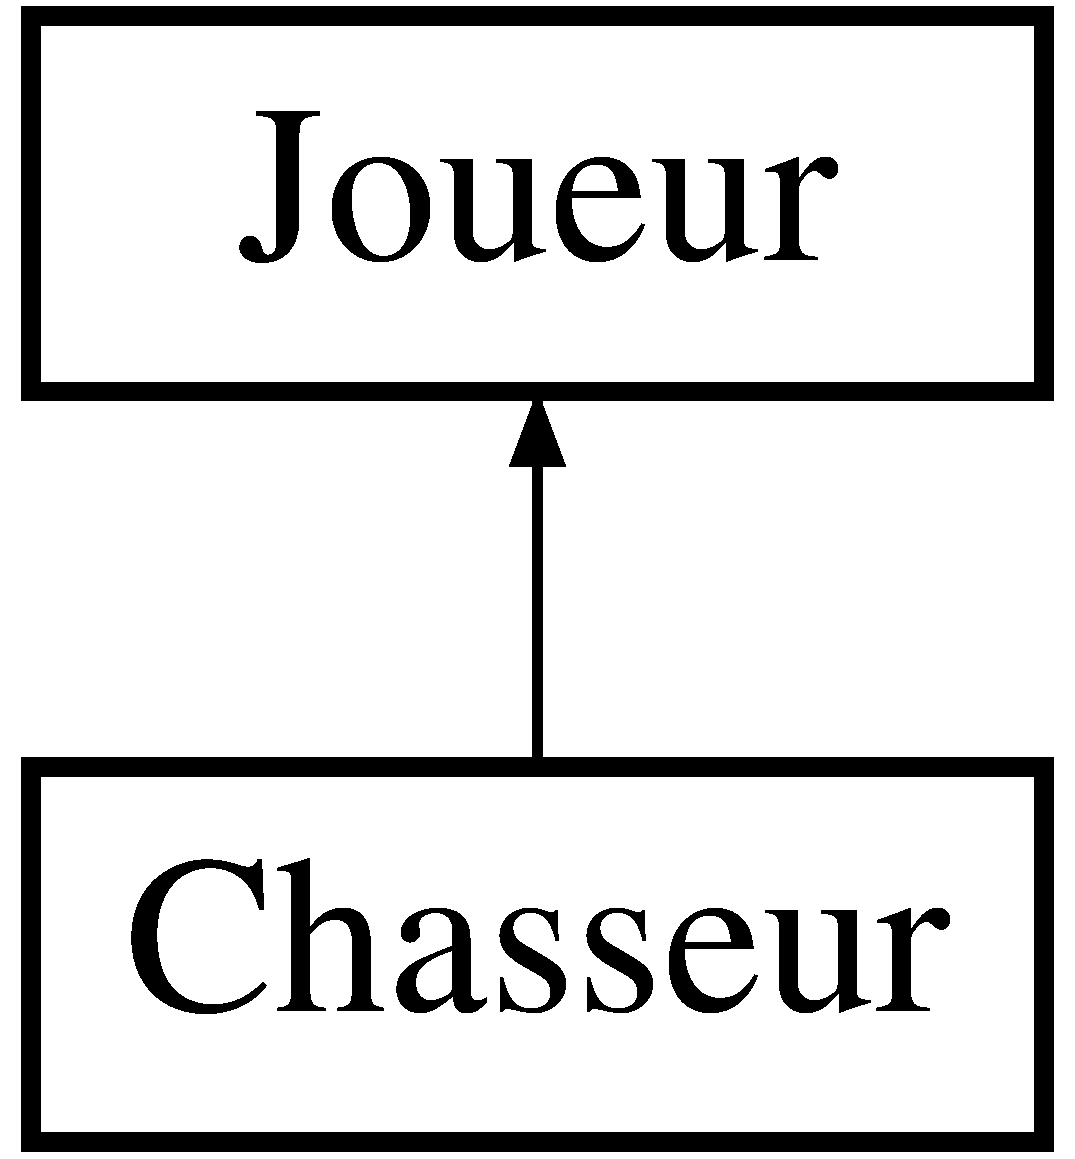
\includegraphics[height=2.000000cm]{class_chasseur}
\end{center}
\end{figure}
\subsection*{Fonctions membres publiques}
\begin{DoxyCompactItemize}
\item 
\hyperlink{class_chasseur_af4bca087f4380663c19cd91cf373cf50}{Chasseur} (std\-::string nom, std\-::string fichier)
\item 
\hyperlink{class_chasseur_a0a2966005d679a141a3da9beeba165fc}{$\sim$\-Chasseur} ()
\end{DoxyCompactItemize}


\subsection{Description détaillée}
Fichier \hyperlink{_chasseur_8hpp}{Chasseur.\-hpp} \begin{DoxyAuthor}{Auteur}
Pierre Gaultier \& Theo Dolez 
\end{DoxyAuthor}


\subsection{Documentation des constructeurs et destructeur}
\hypertarget{class_chasseur_af4bca087f4380663c19cd91cf373cf50}{\index{Chasseur@{Chasseur}!Chasseur@{Chasseur}}
\index{Chasseur@{Chasseur}!Chasseur@{Chasseur}}
\subsubsection[{Chasseur}]{\setlength{\rightskip}{0pt plus 5cm}Chasseur\-::\-Chasseur (
\begin{DoxyParamCaption}
\item[{std\-::string}]{nom, }
\item[{std\-::string}]{fichier}
\end{DoxyParamCaption}
)}}\label{class_chasseur_af4bca087f4380663c19cd91cf373cf50}
Constructeur qui associe au chasseur le comportement du pouvoir du chasseur \hypertarget{class_chasseur_a0a2966005d679a141a3da9beeba165fc}{\index{Chasseur@{Chasseur}!$\sim$\-Chasseur@{$\sim$\-Chasseur}}
\index{$\sim$\-Chasseur@{$\sim$\-Chasseur}!Chasseur@{Chasseur}}
\subsubsection[{$\sim$\-Chasseur}]{\setlength{\rightskip}{0pt plus 5cm}Chasseur\-::$\sim$\-Chasseur (
\begin{DoxyParamCaption}
{}
\end{DoxyParamCaption}
)}}\label{class_chasseur_a0a2966005d679a141a3da9beeba165fc}
Destructeur 

La documentation de cette classe a été générée à partir des fichiers suivants \-:\begin{DoxyCompactItemize}
\item 
include/\-Modele/\-Joueur/\hyperlink{_chasseur_8hpp}{Chasseur.\-hpp}\item 
src/\-Modele/\-Joueur/\hyperlink{_chasseur_8cpp}{Chasseur.\-cpp}\end{DoxyCompactItemize}

\hypertarget{class_comportement_pouvoir}{\section{Référence de la classe Comportement\-Pouvoir}
\label{class_comportement_pouvoir}\index{Comportement\-Pouvoir@{Comportement\-Pouvoir}}
}


{\ttfamily \#include $<$Comportement\-Pouvoir.\-hpp$>$}

Graphe d'héritage de Comportement\-Pouvoir\-:\begin{figure}[H]
\begin{center}
\leavevmode
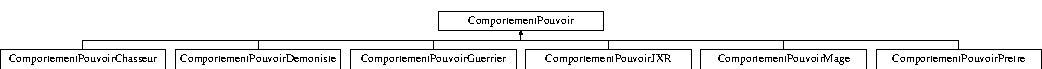
\includegraphics[height=0.924092cm]{class_comportement_pouvoir}
\end{center}
\end{figure}
\subsection*{Fonctions membres publiques}
\begin{DoxyCompactItemize}
\item 
virtual \hyperlink{class_comportement_pouvoir_ab47f80950505addd86dcbdc660f687af}{$\sim$\-Comportement\-Pouvoir} ()
\item 
virtual void \hyperlink{class_comportement_pouvoir_a8b8f4e753291ab73ab0016106f3948ff}{pouvoir} ()=0
\end{DoxyCompactItemize}


\subsection{Description détaillée}
Fichier \hyperlink{class_comportement_pouvoir}{Comportement\-Pouvoir} \begin{DoxyAuthor}{Auteur}
Pierre Gaultier \& Theo Dolez 
\end{DoxyAuthor}


\subsection{Documentation des constructeurs et destructeur}
\hypertarget{class_comportement_pouvoir_ab47f80950505addd86dcbdc660f687af}{\index{Comportement\-Pouvoir@{Comportement\-Pouvoir}!$\sim$\-Comportement\-Pouvoir@{$\sim$\-Comportement\-Pouvoir}}
\index{$\sim$\-Comportement\-Pouvoir@{$\sim$\-Comportement\-Pouvoir}!ComportementPouvoir@{Comportement\-Pouvoir}}
\subsubsection[{$\sim$\-Comportement\-Pouvoir}]{\setlength{\rightskip}{0pt plus 5cm}virtual Comportement\-Pouvoir\-::$\sim$\-Comportement\-Pouvoir (
\begin{DoxyParamCaption}
{}
\end{DoxyParamCaption}
)\hspace{0.3cm}{\ttfamily [inline]}, {\ttfamily [virtual]}}}\label{class_comportement_pouvoir_ab47f80950505addd86dcbdc660f687af}


\subsection{Documentation des fonctions membres}
\hypertarget{class_comportement_pouvoir_a8b8f4e753291ab73ab0016106f3948ff}{\index{Comportement\-Pouvoir@{Comportement\-Pouvoir}!pouvoir@{pouvoir}}
\index{pouvoir@{pouvoir}!ComportementPouvoir@{Comportement\-Pouvoir}}
\subsubsection[{pouvoir}]{\setlength{\rightskip}{0pt plus 5cm}virtual void Comportement\-Pouvoir\-::pouvoir (
\begin{DoxyParamCaption}
{}
\end{DoxyParamCaption}
)\hspace{0.3cm}{\ttfamily [pure virtual]}}}\label{class_comportement_pouvoir_a8b8f4e753291ab73ab0016106f3948ff}


Implémenté dans \hyperlink{class_comportement_pouvoir_j_x_r_a3d40cb49543bd69accaa1ddfb09aa9cc}{Comportement\-Pouvoir\-J\-X\-R}, \hyperlink{class_comportement_pouvoir_mage_a8a85b640972603a96f87222306e57e7d}{Comportement\-Pouvoir\-Mage}, \hyperlink{class_comportement_pouvoir_pretre_a24e87d9b2cb5ab4116d67ace5d3c9687}{Comportement\-Pouvoir\-Pretre}, \hyperlink{class_comportement_pouvoir_chasseur_a334058c088f33d706f636cadd97150da}{Comportement\-Pouvoir\-Chasseur}, \hyperlink{class_comportement_pouvoir_demoniste_a85abc906021128b61ba1c292921c411d}{Comportement\-Pouvoir\-Demoniste}, et \hyperlink{class_comportement_pouvoir_guerrier_a2747bbff54360379e100aa62254a2a79}{Comportement\-Pouvoir\-Guerrier}.



La documentation de cette classe a été générée à partir du fichier suivant \-:\begin{DoxyCompactItemize}
\item 
include/\-Controleur/\-Comportement\-Pouvoir/\hyperlink{_comportement_pouvoir_8hpp}{Comportement\-Pouvoir.\-hpp}\end{DoxyCompactItemize}

\hypertarget{class_comportement_pouvoir_chasseur}{\section{Référence de la classe Comportement\-Pouvoir\-Chasseur}
\label{class_comportement_pouvoir_chasseur}\index{Comportement\-Pouvoir\-Chasseur@{Comportement\-Pouvoir\-Chasseur}}
}


{\ttfamily \#include $<$Comportement\-Pouvoir\-Chasseur.\-hpp$>$}

Graphe d'héritage de Comportement\-Pouvoir\-Chasseur\-:\begin{figure}[H]
\begin{center}
\leavevmode
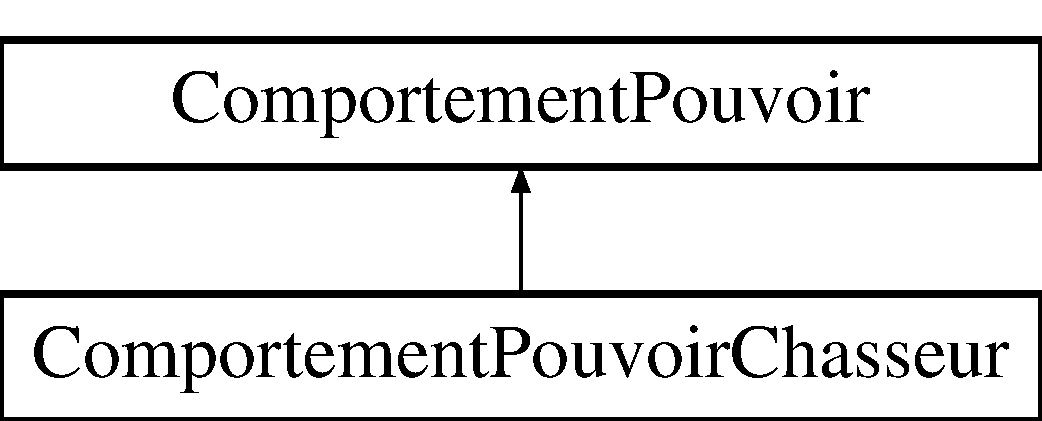
\includegraphics[height=2.000000cm]{class_comportement_pouvoir_chasseur}
\end{center}
\end{figure}
\subsection*{Fonctions membres publiques}
\begin{DoxyCompactItemize}
\item 
\hyperlink{class_comportement_pouvoir_chasseur_a051c87d077549a7edb5eb1e8c9944aff}{Comportement\-Pouvoir\-Chasseur} (\hyperlink{class_joueur}{Joueur} $\ast$j)
\item 
\hyperlink{class_comportement_pouvoir_chasseur_aaad834dea06fd69007e220d611927091}{$\sim$\-Comportement\-Pouvoir\-Chasseur} ()
\item 
void \hyperlink{class_comportement_pouvoir_chasseur_a334058c088f33d706f636cadd97150da}{pouvoir} ()
\end{DoxyCompactItemize}


\subsection{Description détaillée}
Fichier \hyperlink{class_comportement_pouvoir_chasseur}{Comportement\-Pouvoir\-Chasseur} \begin{DoxyAuthor}{Auteur}
Pierre Gaultier \& Theo Dolez 
\end{DoxyAuthor}


\subsection{Documentation des constructeurs et destructeur}
\hypertarget{class_comportement_pouvoir_chasseur_a051c87d077549a7edb5eb1e8c9944aff}{\index{Comportement\-Pouvoir\-Chasseur@{Comportement\-Pouvoir\-Chasseur}!Comportement\-Pouvoir\-Chasseur@{Comportement\-Pouvoir\-Chasseur}}
\index{Comportement\-Pouvoir\-Chasseur@{Comportement\-Pouvoir\-Chasseur}!ComportementPouvoirChasseur@{Comportement\-Pouvoir\-Chasseur}}
\subsubsection[{Comportement\-Pouvoir\-Chasseur}]{\setlength{\rightskip}{0pt plus 5cm}Comportement\-Pouvoir\-Chasseur\-::\-Comportement\-Pouvoir\-Chasseur (
\begin{DoxyParamCaption}
\item[{{\bf Joueur} $\ast$}]{j}
\end{DoxyParamCaption}
)}}\label{class_comportement_pouvoir_chasseur_a051c87d077549a7edb5eb1e8c9944aff}
Constructeur. \hypertarget{class_comportement_pouvoir_chasseur_aaad834dea06fd69007e220d611927091}{\index{Comportement\-Pouvoir\-Chasseur@{Comportement\-Pouvoir\-Chasseur}!$\sim$\-Comportement\-Pouvoir\-Chasseur@{$\sim$\-Comportement\-Pouvoir\-Chasseur}}
\index{$\sim$\-Comportement\-Pouvoir\-Chasseur@{$\sim$\-Comportement\-Pouvoir\-Chasseur}!ComportementPouvoirChasseur@{Comportement\-Pouvoir\-Chasseur}}
\subsubsection[{$\sim$\-Comportement\-Pouvoir\-Chasseur}]{\setlength{\rightskip}{0pt plus 5cm}Comportement\-Pouvoir\-Chasseur\-::$\sim$\-Comportement\-Pouvoir\-Chasseur (
\begin{DoxyParamCaption}
{}
\end{DoxyParamCaption}
)}}\label{class_comportement_pouvoir_chasseur_aaad834dea06fd69007e220d611927091}
Destructeur. 

\subsection{Documentation des fonctions membres}
\hypertarget{class_comportement_pouvoir_chasseur_a334058c088f33d706f636cadd97150da}{\index{Comportement\-Pouvoir\-Chasseur@{Comportement\-Pouvoir\-Chasseur}!pouvoir@{pouvoir}}
\index{pouvoir@{pouvoir}!ComportementPouvoirChasseur@{Comportement\-Pouvoir\-Chasseur}}
\subsubsection[{pouvoir}]{\setlength{\rightskip}{0pt plus 5cm}void Comportement\-Pouvoir\-Chasseur\-::pouvoir (
\begin{DoxyParamCaption}
{}
\end{DoxyParamCaption}
)\hspace{0.3cm}{\ttfamily [virtual]}}}\label{class_comportement_pouvoir_chasseur_a334058c088f33d706f636cadd97150da}
Methode qui applique le pouvoir heroique du \hyperlink{class_chasseur}{Chasseur} 

Implémente \hyperlink{class_comportement_pouvoir_a8b8f4e753291ab73ab0016106f3948ff}{Comportement\-Pouvoir}.



La documentation de cette classe a été générée à partir des fichiers suivants \-:\begin{DoxyCompactItemize}
\item 
include/\-Controleur/\-Comportement\-Pouvoir/\hyperlink{_comportement_pouvoir_chasseur_8hpp}{Comportement\-Pouvoir\-Chasseur.\-hpp}\item 
src/\-Controleur/\-Comportement\-Pouvoir/\hyperlink{_comportement_pouvoir_chasseur_8cpp}{Comportement\-Pouvoir\-Chasseur.\-cpp}\end{DoxyCompactItemize}

\hypertarget{class_comportement_pouvoir_demoniste}{\section{Référence de la classe Comportement\-Pouvoir\-Demoniste}
\label{class_comportement_pouvoir_demoniste}\index{Comportement\-Pouvoir\-Demoniste@{Comportement\-Pouvoir\-Demoniste}}
}


{\ttfamily \#include $<$Comportement\-Pouvoir\-Demoniste.\-hpp$>$}

Graphe d'héritage de Comportement\-Pouvoir\-Demoniste\-:\begin{figure}[H]
\begin{center}
\leavevmode
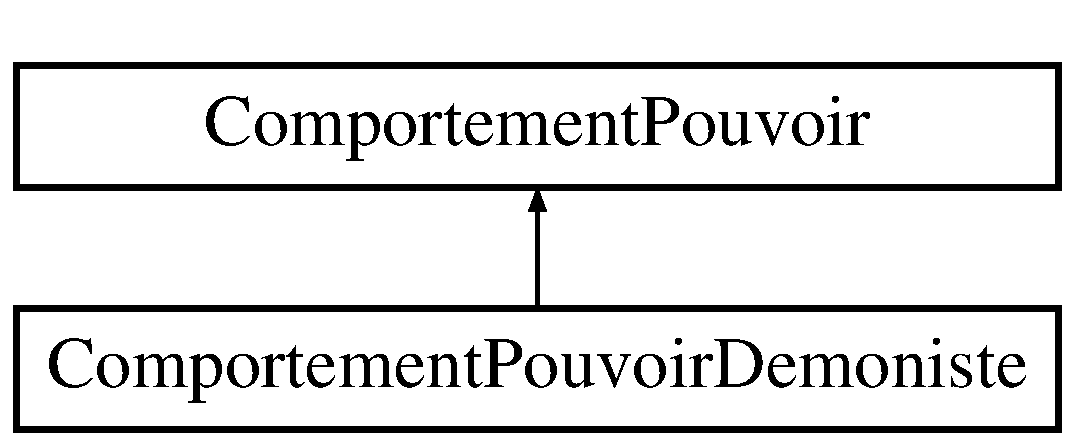
\includegraphics[height=2.000000cm]{class_comportement_pouvoir_demoniste}
\end{center}
\end{figure}
\subsection*{Fonctions membres publiques}
\begin{DoxyCompactItemize}
\item 
\hyperlink{class_comportement_pouvoir_demoniste_a1f6b2e5586c6c0e48cd2d88be22e730a}{Comportement\-Pouvoir\-Demoniste} (\hyperlink{class_joueur}{Joueur} $\ast$j)
\item 
\hyperlink{class_comportement_pouvoir_demoniste_a95cd36e0a6e6b10c9931ca1f4b9daad8}{$\sim$\-Comportement\-Pouvoir\-Demoniste} ()
\item 
void \hyperlink{class_comportement_pouvoir_demoniste_a85abc906021128b61ba1c292921c411d}{pouvoir} ()
\end{DoxyCompactItemize}


\subsection{Description détaillée}
Fichier \hyperlink{class_comportement_pouvoir_demoniste}{Comportement\-Pouvoir\-Demoniste} \begin{DoxyAuthor}{Auteur}
Pierre Gaultier \& Theo Dolez 
\end{DoxyAuthor}


\subsection{Documentation des constructeurs et destructeur}
\hypertarget{class_comportement_pouvoir_demoniste_a1f6b2e5586c6c0e48cd2d88be22e730a}{\index{Comportement\-Pouvoir\-Demoniste@{Comportement\-Pouvoir\-Demoniste}!Comportement\-Pouvoir\-Demoniste@{Comportement\-Pouvoir\-Demoniste}}
\index{Comportement\-Pouvoir\-Demoniste@{Comportement\-Pouvoir\-Demoniste}!ComportementPouvoirDemoniste@{Comportement\-Pouvoir\-Demoniste}}
\subsubsection[{Comportement\-Pouvoir\-Demoniste}]{\setlength{\rightskip}{0pt plus 5cm}Comportement\-Pouvoir\-Demoniste\-::\-Comportement\-Pouvoir\-Demoniste (
\begin{DoxyParamCaption}
\item[{{\bf Joueur} $\ast$}]{j}
\end{DoxyParamCaption}
)}}\label{class_comportement_pouvoir_demoniste_a1f6b2e5586c6c0e48cd2d88be22e730a}
Constructeur. \hypertarget{class_comportement_pouvoir_demoniste_a95cd36e0a6e6b10c9931ca1f4b9daad8}{\index{Comportement\-Pouvoir\-Demoniste@{Comportement\-Pouvoir\-Demoniste}!$\sim$\-Comportement\-Pouvoir\-Demoniste@{$\sim$\-Comportement\-Pouvoir\-Demoniste}}
\index{$\sim$\-Comportement\-Pouvoir\-Demoniste@{$\sim$\-Comportement\-Pouvoir\-Demoniste}!ComportementPouvoirDemoniste@{Comportement\-Pouvoir\-Demoniste}}
\subsubsection[{$\sim$\-Comportement\-Pouvoir\-Demoniste}]{\setlength{\rightskip}{0pt plus 5cm}Comportement\-Pouvoir\-Demoniste\-::$\sim$\-Comportement\-Pouvoir\-Demoniste (
\begin{DoxyParamCaption}
{}
\end{DoxyParamCaption}
)}}\label{class_comportement_pouvoir_demoniste_a95cd36e0a6e6b10c9931ca1f4b9daad8}
Destructeur. 

\subsection{Documentation des fonctions membres}
\hypertarget{class_comportement_pouvoir_demoniste_a85abc906021128b61ba1c292921c411d}{\index{Comportement\-Pouvoir\-Demoniste@{Comportement\-Pouvoir\-Demoniste}!pouvoir@{pouvoir}}
\index{pouvoir@{pouvoir}!ComportementPouvoirDemoniste@{Comportement\-Pouvoir\-Demoniste}}
\subsubsection[{pouvoir}]{\setlength{\rightskip}{0pt plus 5cm}void Comportement\-Pouvoir\-Demoniste\-::pouvoir (
\begin{DoxyParamCaption}
{}
\end{DoxyParamCaption}
)\hspace{0.3cm}{\ttfamily [virtual]}}}\label{class_comportement_pouvoir_demoniste_a85abc906021128b61ba1c292921c411d}
Methode qui applique le pouvoir heroique du \hyperlink{class_demoniste}{Demoniste} 

Implémente \hyperlink{class_comportement_pouvoir_a8b8f4e753291ab73ab0016106f3948ff}{Comportement\-Pouvoir}.



La documentation de cette classe a été générée à partir des fichiers suivants \-:\begin{DoxyCompactItemize}
\item 
include/\-Controleur/\-Comportement\-Pouvoir/\hyperlink{_comportement_pouvoir_demoniste_8hpp}{Comportement\-Pouvoir\-Demoniste.\-hpp}\item 
src/\-Controleur/\-Comportement\-Pouvoir/\hyperlink{_comportement_pouvoir_demoniste_8cpp}{Comportement\-Pouvoir\-Demoniste.\-cpp}\end{DoxyCompactItemize}

\hypertarget{class_comportement_pouvoir_guerrier}{\section{Référence de la classe Comportement\-Pouvoir\-Guerrier}
\label{class_comportement_pouvoir_guerrier}\index{Comportement\-Pouvoir\-Guerrier@{Comportement\-Pouvoir\-Guerrier}}
}


{\ttfamily \#include $<$Comportement\-Pouvoir\-Guerrier.\-hpp$>$}

Graphe d'héritage de Comportement\-Pouvoir\-Guerrier\-:\begin{figure}[H]
\begin{center}
\leavevmode
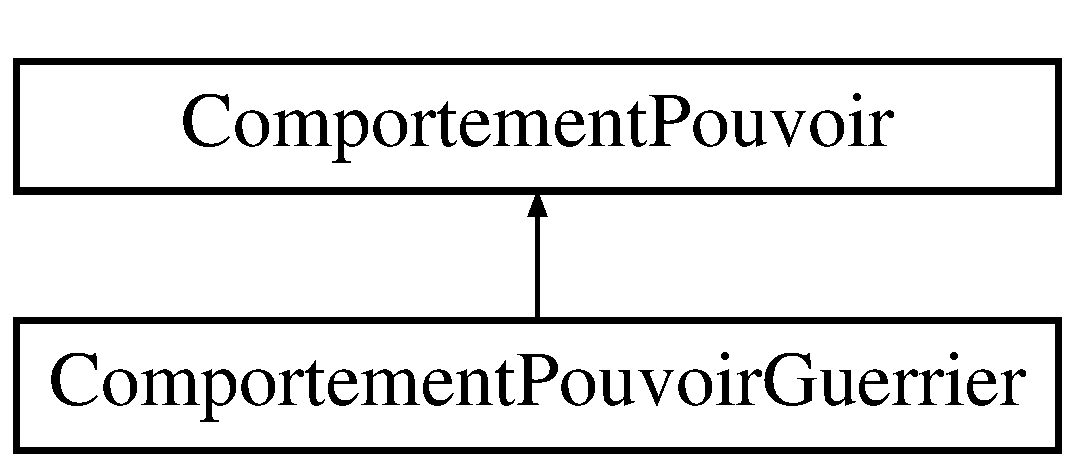
\includegraphics[height=2.000000cm]{class_comportement_pouvoir_guerrier}
\end{center}
\end{figure}
\subsection*{Fonctions membres publiques}
\begin{DoxyCompactItemize}
\item 
\hyperlink{class_comportement_pouvoir_guerrier_a5b4e19698e98c3d7a58a3859c6ca5118}{Comportement\-Pouvoir\-Guerrier} (\hyperlink{class_joueur}{Joueur} $\ast$j)
\item 
\hyperlink{class_comportement_pouvoir_guerrier_ae5113657a16d91283b311f18aa32b1e9}{$\sim$\-Comportement\-Pouvoir\-Guerrier} ()
\item 
void \hyperlink{class_comportement_pouvoir_guerrier_a2747bbff54360379e100aa62254a2a79}{pouvoir} ()
\end{DoxyCompactItemize}


\subsection{Description détaillée}
Fichier \hyperlink{class_comportement_pouvoir_guerrier}{Comportement\-Pouvoir\-Guerrier} \begin{DoxyAuthor}{Auteur}
Pierre Gaultier \& Theo Dolez 
\end{DoxyAuthor}


\subsection{Documentation des constructeurs et destructeur}
\hypertarget{class_comportement_pouvoir_guerrier_a5b4e19698e98c3d7a58a3859c6ca5118}{\index{Comportement\-Pouvoir\-Guerrier@{Comportement\-Pouvoir\-Guerrier}!Comportement\-Pouvoir\-Guerrier@{Comportement\-Pouvoir\-Guerrier}}
\index{Comportement\-Pouvoir\-Guerrier@{Comportement\-Pouvoir\-Guerrier}!ComportementPouvoirGuerrier@{Comportement\-Pouvoir\-Guerrier}}
\subsubsection[{Comportement\-Pouvoir\-Guerrier}]{\setlength{\rightskip}{0pt plus 5cm}Comportement\-Pouvoir\-Guerrier\-::\-Comportement\-Pouvoir\-Guerrier (
\begin{DoxyParamCaption}
\item[{{\bf Joueur} $\ast$}]{j}
\end{DoxyParamCaption}
)}}\label{class_comportement_pouvoir_guerrier_a5b4e19698e98c3d7a58a3859c6ca5118}
Constructeur. \hypertarget{class_comportement_pouvoir_guerrier_ae5113657a16d91283b311f18aa32b1e9}{\index{Comportement\-Pouvoir\-Guerrier@{Comportement\-Pouvoir\-Guerrier}!$\sim$\-Comportement\-Pouvoir\-Guerrier@{$\sim$\-Comportement\-Pouvoir\-Guerrier}}
\index{$\sim$\-Comportement\-Pouvoir\-Guerrier@{$\sim$\-Comportement\-Pouvoir\-Guerrier}!ComportementPouvoirGuerrier@{Comportement\-Pouvoir\-Guerrier}}
\subsubsection[{$\sim$\-Comportement\-Pouvoir\-Guerrier}]{\setlength{\rightskip}{0pt plus 5cm}Comportement\-Pouvoir\-Guerrier\-::$\sim$\-Comportement\-Pouvoir\-Guerrier (
\begin{DoxyParamCaption}
{}
\end{DoxyParamCaption}
)}}\label{class_comportement_pouvoir_guerrier_ae5113657a16d91283b311f18aa32b1e9}
Destructeur. 

\subsection{Documentation des fonctions membres}
\hypertarget{class_comportement_pouvoir_guerrier_a2747bbff54360379e100aa62254a2a79}{\index{Comportement\-Pouvoir\-Guerrier@{Comportement\-Pouvoir\-Guerrier}!pouvoir@{pouvoir}}
\index{pouvoir@{pouvoir}!ComportementPouvoirGuerrier@{Comportement\-Pouvoir\-Guerrier}}
\subsubsection[{pouvoir}]{\setlength{\rightskip}{0pt plus 5cm}void Comportement\-Pouvoir\-Guerrier\-::pouvoir (
\begin{DoxyParamCaption}
{}
\end{DoxyParamCaption}
)\hspace{0.3cm}{\ttfamily [virtual]}}}\label{class_comportement_pouvoir_guerrier_a2747bbff54360379e100aa62254a2a79}
Methode qui applique le pouvoir heroique du guerrier 

Implémente \hyperlink{class_comportement_pouvoir_a8b8f4e753291ab73ab0016106f3948ff}{Comportement\-Pouvoir}.



La documentation de cette classe a été générée à partir des fichiers suivants \-:\begin{DoxyCompactItemize}
\item 
include/\-Controleur/\-Comportement\-Pouvoir/\hyperlink{_comportement_pouvoir_guerrier_8hpp}{Comportement\-Pouvoir\-Guerrier.\-hpp}\item 
src/\-Controleur/\-Comportement\-Pouvoir/\hyperlink{_comportement_pouvoir_guerrier_8cpp}{Comportement\-Pouvoir\-Guerrier.\-cpp}\end{DoxyCompactItemize}

\hypertarget{class_comportement_pouvoir_j_x_r}{\section{Référence de la classe Comportement\-Pouvoir\-J\-X\-R}
\label{class_comportement_pouvoir_j_x_r}\index{Comportement\-Pouvoir\-J\-X\-R@{Comportement\-Pouvoir\-J\-X\-R}}
}


{\ttfamily \#include $<$Comportement\-Pouvoir\-J\-X\-R.\-hpp$>$}

Graphe d'héritage de Comportement\-Pouvoir\-J\-X\-R\-:\begin{figure}[H]
\begin{center}
\leavevmode
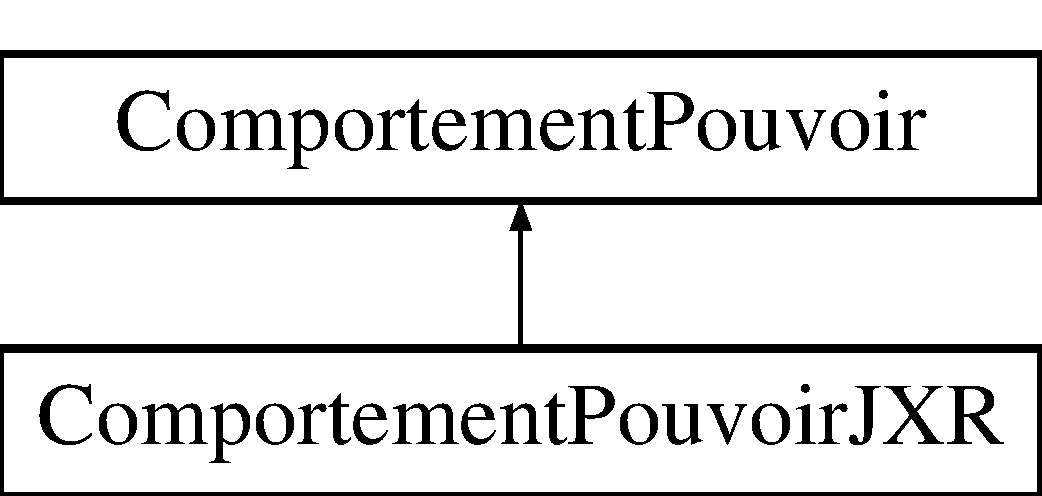
\includegraphics[height=2.000000cm]{class_comportement_pouvoir_j_x_r}
\end{center}
\end{figure}
\subsection*{Fonctions membres publiques}
\begin{DoxyCompactItemize}
\item 
\hyperlink{class_comportement_pouvoir_j_x_r_a6bfa37111b1d6add5cabd1c5a433291b}{Comportement\-Pouvoir\-J\-X\-R} (\hyperlink{class_joueur}{Joueur} $\ast$j)
\item 
\hyperlink{class_comportement_pouvoir_j_x_r_a60e6ba18e25818261a5c11bd6780db10}{$\sim$\-Comportement\-Pouvoir\-J\-X\-R} ()
\item 
void \hyperlink{class_comportement_pouvoir_j_x_r_a3d40cb49543bd69accaa1ddfb09aa9cc}{pouvoir} ()
\end{DoxyCompactItemize}


\subsection{Description détaillée}
Fichier \hyperlink{class_comportement_pouvoir_j_x_r}{Comportement\-Pouvoir\-J\-X\-R} \begin{DoxyAuthor}{Auteur}
Pierre Gaultier \& Theo Dolez 
\end{DoxyAuthor}


\subsection{Documentation des constructeurs et destructeur}
\hypertarget{class_comportement_pouvoir_j_x_r_a6bfa37111b1d6add5cabd1c5a433291b}{\index{Comportement\-Pouvoir\-J\-X\-R@{Comportement\-Pouvoir\-J\-X\-R}!Comportement\-Pouvoir\-J\-X\-R@{Comportement\-Pouvoir\-J\-X\-R}}
\index{Comportement\-Pouvoir\-J\-X\-R@{Comportement\-Pouvoir\-J\-X\-R}!ComportementPouvoirJXR@{Comportement\-Pouvoir\-J\-X\-R}}
\subsubsection[{Comportement\-Pouvoir\-J\-X\-R}]{\setlength{\rightskip}{0pt plus 5cm}Comportement\-Pouvoir\-J\-X\-R\-::\-Comportement\-Pouvoir\-J\-X\-R (
\begin{DoxyParamCaption}
\item[{{\bf Joueur} $\ast$}]{j}
\end{DoxyParamCaption}
)}}\label{class_comportement_pouvoir_j_x_r_a6bfa37111b1d6add5cabd1c5a433291b}
Constructeur. \hypertarget{class_comportement_pouvoir_j_x_r_a60e6ba18e25818261a5c11bd6780db10}{\index{Comportement\-Pouvoir\-J\-X\-R@{Comportement\-Pouvoir\-J\-X\-R}!$\sim$\-Comportement\-Pouvoir\-J\-X\-R@{$\sim$\-Comportement\-Pouvoir\-J\-X\-R}}
\index{$\sim$\-Comportement\-Pouvoir\-J\-X\-R@{$\sim$\-Comportement\-Pouvoir\-J\-X\-R}!ComportementPouvoirJXR@{Comportement\-Pouvoir\-J\-X\-R}}
\subsubsection[{$\sim$\-Comportement\-Pouvoir\-J\-X\-R}]{\setlength{\rightskip}{0pt plus 5cm}Comportement\-Pouvoir\-J\-X\-R\-::$\sim$\-Comportement\-Pouvoir\-J\-X\-R (
\begin{DoxyParamCaption}
{}
\end{DoxyParamCaption}
)}}\label{class_comportement_pouvoir_j_x_r_a60e6ba18e25818261a5c11bd6780db10}
Destructeur 

\subsection{Documentation des fonctions membres}
\hypertarget{class_comportement_pouvoir_j_x_r_a3d40cb49543bd69accaa1ddfb09aa9cc}{\index{Comportement\-Pouvoir\-J\-X\-R@{Comportement\-Pouvoir\-J\-X\-R}!pouvoir@{pouvoir}}
\index{pouvoir@{pouvoir}!ComportementPouvoirJXR@{Comportement\-Pouvoir\-J\-X\-R}}
\subsubsection[{pouvoir}]{\setlength{\rightskip}{0pt plus 5cm}void Comportement\-Pouvoir\-J\-X\-R\-::pouvoir (
\begin{DoxyParamCaption}
{}
\end{DoxyParamCaption}
)\hspace{0.3cm}{\ttfamily [virtual]}}}\label{class_comportement_pouvoir_j_x_r_a3d40cb49543bd69accaa1ddfb09aa9cc}
Methode qui applique le pouvoir heroique de \hyperlink{class_j_x_r}{J\-X\-R} 

Implémente \hyperlink{class_comportement_pouvoir_a8b8f4e753291ab73ab0016106f3948ff}{Comportement\-Pouvoir}.



La documentation de cette classe a été générée à partir des fichiers suivants \-:\begin{DoxyCompactItemize}
\item 
include/\-Controleur/\-Comportement\-Pouvoir/\hyperlink{_comportement_pouvoir_j_x_r_8hpp}{Comportement\-Pouvoir\-J\-X\-R.\-hpp}\item 
src/\-Controleur/\-Comportement\-Pouvoir/\hyperlink{_comportement_pouvoir_j_x_r_8cpp}{Comportement\-Pouvoir\-J\-X\-R.\-cpp}\end{DoxyCompactItemize}

\hypertarget{class_comportement_pouvoir_mage}{\section{Référence de la classe Comportement\-Pouvoir\-Mage}
\label{class_comportement_pouvoir_mage}\index{Comportement\-Pouvoir\-Mage@{Comportement\-Pouvoir\-Mage}}
}


{\ttfamily \#include $<$Comportement\-Pouvoir\-Mage.\-hpp$>$}

Graphe d'héritage de Comportement\-Pouvoir\-Mage\-:\begin{figure}[H]
\begin{center}
\leavevmode
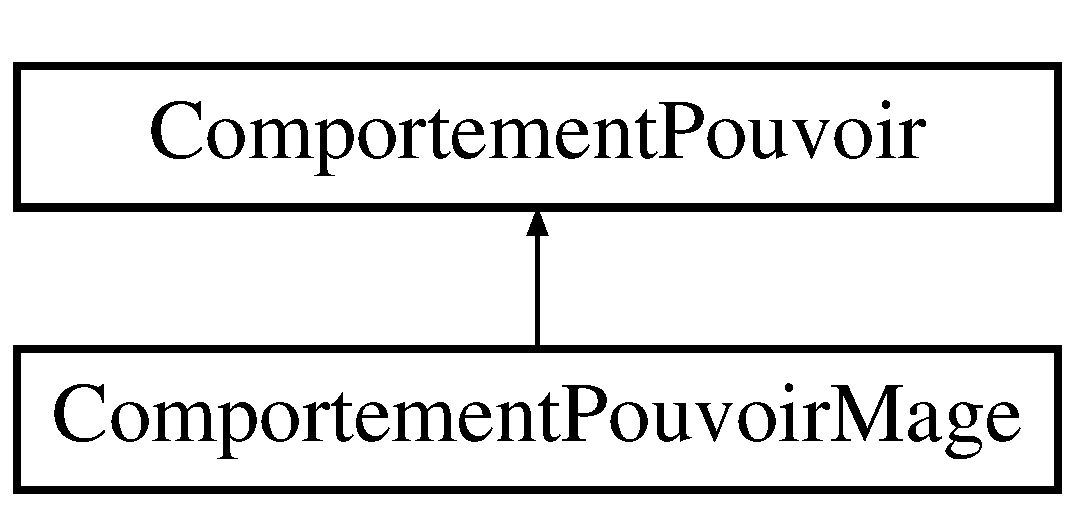
\includegraphics[height=2.000000cm]{class_comportement_pouvoir_mage}
\end{center}
\end{figure}
\subsection*{Fonctions membres publiques}
\begin{DoxyCompactItemize}
\item 
\hyperlink{class_comportement_pouvoir_mage_a981ec14dbba67cb5d5c709d84fd23d1d}{Comportement\-Pouvoir\-Mage} (\hyperlink{class_joueur}{Joueur} $\ast$j)
\item 
\hyperlink{class_comportement_pouvoir_mage_a0eb90adc162f3385ad5962b68a9768b8}{$\sim$\-Comportement\-Pouvoir\-Mage} ()
\item 
void \hyperlink{class_comportement_pouvoir_mage_a8a85b640972603a96f87222306e57e7d}{pouvoir} ()
\end{DoxyCompactItemize}


\subsection{Description détaillée}
Fichier \hyperlink{class_comportement_pouvoir_mage}{Comportement\-Pouvoir\-Mage} \begin{DoxyAuthor}{Auteur}
Pierre Gaultier \& Theo Dolez 
\end{DoxyAuthor}


\subsection{Documentation des constructeurs et destructeur}
\hypertarget{class_comportement_pouvoir_mage_a981ec14dbba67cb5d5c709d84fd23d1d}{\index{Comportement\-Pouvoir\-Mage@{Comportement\-Pouvoir\-Mage}!Comportement\-Pouvoir\-Mage@{Comportement\-Pouvoir\-Mage}}
\index{Comportement\-Pouvoir\-Mage@{Comportement\-Pouvoir\-Mage}!ComportementPouvoirMage@{Comportement\-Pouvoir\-Mage}}
\subsubsection[{Comportement\-Pouvoir\-Mage}]{\setlength{\rightskip}{0pt plus 5cm}Comportement\-Pouvoir\-Mage\-::\-Comportement\-Pouvoir\-Mage (
\begin{DoxyParamCaption}
\item[{{\bf Joueur} $\ast$}]{j}
\end{DoxyParamCaption}
)}}\label{class_comportement_pouvoir_mage_a981ec14dbba67cb5d5c709d84fd23d1d}
Constructeur. \hypertarget{class_comportement_pouvoir_mage_a0eb90adc162f3385ad5962b68a9768b8}{\index{Comportement\-Pouvoir\-Mage@{Comportement\-Pouvoir\-Mage}!$\sim$\-Comportement\-Pouvoir\-Mage@{$\sim$\-Comportement\-Pouvoir\-Mage}}
\index{$\sim$\-Comportement\-Pouvoir\-Mage@{$\sim$\-Comportement\-Pouvoir\-Mage}!ComportementPouvoirMage@{Comportement\-Pouvoir\-Mage}}
\subsubsection[{$\sim$\-Comportement\-Pouvoir\-Mage}]{\setlength{\rightskip}{0pt plus 5cm}Comportement\-Pouvoir\-Mage\-::$\sim$\-Comportement\-Pouvoir\-Mage (
\begin{DoxyParamCaption}
{}
\end{DoxyParamCaption}
)}}\label{class_comportement_pouvoir_mage_a0eb90adc162f3385ad5962b68a9768b8}
Destructeur 

\subsection{Documentation des fonctions membres}
\hypertarget{class_comportement_pouvoir_mage_a8a85b640972603a96f87222306e57e7d}{\index{Comportement\-Pouvoir\-Mage@{Comportement\-Pouvoir\-Mage}!pouvoir@{pouvoir}}
\index{pouvoir@{pouvoir}!ComportementPouvoirMage@{Comportement\-Pouvoir\-Mage}}
\subsubsection[{pouvoir}]{\setlength{\rightskip}{0pt plus 5cm}void Comportement\-Pouvoir\-Mage\-::pouvoir (
\begin{DoxyParamCaption}
{}
\end{DoxyParamCaption}
)\hspace{0.3cm}{\ttfamily [virtual]}}}\label{class_comportement_pouvoir_mage_a8a85b640972603a96f87222306e57e7d}
Methode qui applique le pouvoir heroique du \hyperlink{class_mage}{Mage} 

Implémente \hyperlink{class_comportement_pouvoir_a8b8f4e753291ab73ab0016106f3948ff}{Comportement\-Pouvoir}.



La documentation de cette classe a été générée à partir des fichiers suivants \-:\begin{DoxyCompactItemize}
\item 
include/\-Controleur/\-Comportement\-Pouvoir/\hyperlink{_comportement_pouvoir_mage_8hpp}{Comportement\-Pouvoir\-Mage.\-hpp}\item 
src/\-Controleur/\-Comportement\-Pouvoir/\hyperlink{_comportement_pouvoir_mage_8cpp}{Comportement\-Pouvoir\-Mage.\-cpp}\end{DoxyCompactItemize}

\hypertarget{class_comportement_pouvoir_pretre}{\section{Référence de la classe Comportement\-Pouvoir\-Pretre}
\label{class_comportement_pouvoir_pretre}\index{Comportement\-Pouvoir\-Pretre@{Comportement\-Pouvoir\-Pretre}}
}


{\ttfamily \#include $<$Comportement\-Pouvoir\-Pretre.\-hpp$>$}

Graphe d'héritage de Comportement\-Pouvoir\-Pretre\-:\begin{figure}[H]
\begin{center}
\leavevmode
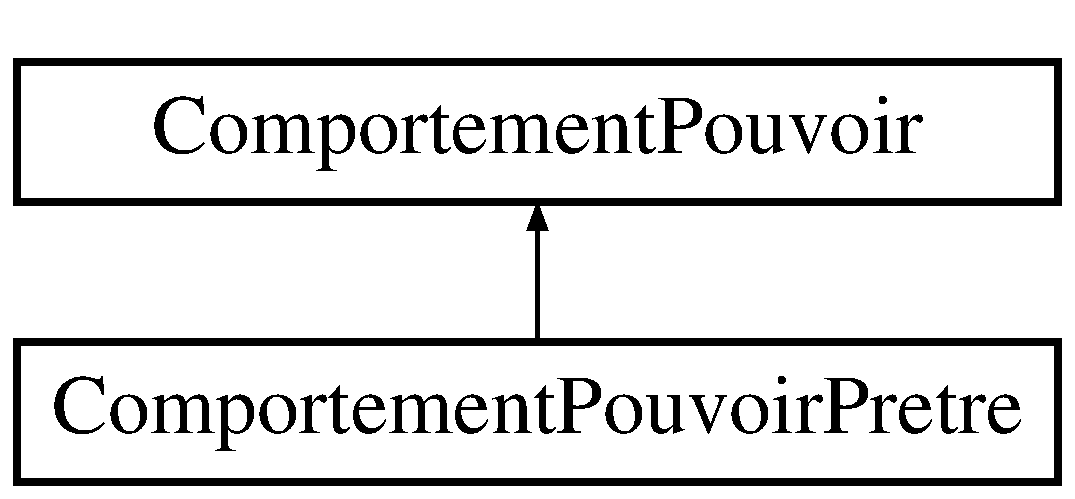
\includegraphics[height=2.000000cm]{class_comportement_pouvoir_pretre}
\end{center}
\end{figure}
\subsection*{Fonctions membres publiques}
\begin{DoxyCompactItemize}
\item 
\hyperlink{class_comportement_pouvoir_pretre_a997a0441eabec5c50a1cfa29d9aabdaa}{Comportement\-Pouvoir\-Pretre} (\hyperlink{class_joueur}{Joueur} $\ast$j)
\item 
\hyperlink{class_comportement_pouvoir_pretre_a5232928218a13a88d8f1d4aecf440147}{$\sim$\-Comportement\-Pouvoir\-Pretre} ()
\item 
void \hyperlink{class_comportement_pouvoir_pretre_a24e87d9b2cb5ab4116d67ace5d3c9687}{pouvoir} ()
\end{DoxyCompactItemize}


\subsection{Description détaillée}
Fichier \hyperlink{class_comportement_pouvoir_pretre}{Comportement\-Pouvoir\-Pretre} \begin{DoxyAuthor}{Auteur}
Pierre Gaultier \& Theo Dolez 
\end{DoxyAuthor}


\subsection{Documentation des constructeurs et destructeur}
\hypertarget{class_comportement_pouvoir_pretre_a997a0441eabec5c50a1cfa29d9aabdaa}{\index{Comportement\-Pouvoir\-Pretre@{Comportement\-Pouvoir\-Pretre}!Comportement\-Pouvoir\-Pretre@{Comportement\-Pouvoir\-Pretre}}
\index{Comportement\-Pouvoir\-Pretre@{Comportement\-Pouvoir\-Pretre}!ComportementPouvoirPretre@{Comportement\-Pouvoir\-Pretre}}
\subsubsection[{Comportement\-Pouvoir\-Pretre}]{\setlength{\rightskip}{0pt plus 5cm}Comportement\-Pouvoir\-Pretre\-::\-Comportement\-Pouvoir\-Pretre (
\begin{DoxyParamCaption}
\item[{{\bf Joueur} $\ast$}]{j}
\end{DoxyParamCaption}
)}}\label{class_comportement_pouvoir_pretre_a997a0441eabec5c50a1cfa29d9aabdaa}
Constructeur. \hypertarget{class_comportement_pouvoir_pretre_a5232928218a13a88d8f1d4aecf440147}{\index{Comportement\-Pouvoir\-Pretre@{Comportement\-Pouvoir\-Pretre}!$\sim$\-Comportement\-Pouvoir\-Pretre@{$\sim$\-Comportement\-Pouvoir\-Pretre}}
\index{$\sim$\-Comportement\-Pouvoir\-Pretre@{$\sim$\-Comportement\-Pouvoir\-Pretre}!ComportementPouvoirPretre@{Comportement\-Pouvoir\-Pretre}}
\subsubsection[{$\sim$\-Comportement\-Pouvoir\-Pretre}]{\setlength{\rightskip}{0pt plus 5cm}Comportement\-Pouvoir\-Pretre\-::$\sim$\-Comportement\-Pouvoir\-Pretre (
\begin{DoxyParamCaption}
{}
\end{DoxyParamCaption}
)}}\label{class_comportement_pouvoir_pretre_a5232928218a13a88d8f1d4aecf440147}
Destructeur 

\subsection{Documentation des fonctions membres}
\hypertarget{class_comportement_pouvoir_pretre_a24e87d9b2cb5ab4116d67ace5d3c9687}{\index{Comportement\-Pouvoir\-Pretre@{Comportement\-Pouvoir\-Pretre}!pouvoir@{pouvoir}}
\index{pouvoir@{pouvoir}!ComportementPouvoirPretre@{Comportement\-Pouvoir\-Pretre}}
\subsubsection[{pouvoir}]{\setlength{\rightskip}{0pt plus 5cm}void Comportement\-Pouvoir\-Pretre\-::pouvoir (
\begin{DoxyParamCaption}
{}
\end{DoxyParamCaption}
)\hspace{0.3cm}{\ttfamily [virtual]}}}\label{class_comportement_pouvoir_pretre_a24e87d9b2cb5ab4116d67ace5d3c9687}
Methode qui applique le pouvoir heroique du \hyperlink{class_pretre}{Pretre} 

Implémente \hyperlink{class_comportement_pouvoir_a8b8f4e753291ab73ab0016106f3948ff}{Comportement\-Pouvoir}.



La documentation de cette classe a été générée à partir des fichiers suivants \-:\begin{DoxyCompactItemize}
\item 
include/\-Controleur/\-Comportement\-Pouvoir/\hyperlink{_comportement_pouvoir_pretre_8hpp}{Comportement\-Pouvoir\-Pretre.\-hpp}\item 
src/\-Controleur/\-Comportement\-Pouvoir/\hyperlink{_comportement_pouvoir_pretre_8cpp}{Comportement\-Pouvoir\-Pretre.\-cpp}\end{DoxyCompactItemize}

\hypertarget{class_deck}{\section{Référence de la classe Deck}
\label{class_deck}\index{Deck@{Deck}}
}


{\ttfamily \#include $<$Deck.\-hpp$>$}

\subsection*{Fonctions membres publiques}
\begin{DoxyCompactItemize}
\item 
\hyperlink{class_deck_abd58d9e32c8bd9fe7a05a12a4882d94c}{Deck} (std\-::string fichier)
\item 
\hyperlink{class_deck_a7d1331cc558c302fdf44e5ae8aae1a95}{$\sim$\-Deck} ()
\item 
int \hyperlink{class_deck_a34272f22ad41d349f7b347c07fd0cbb4}{get\-Taille} ()
\item 
void \hyperlink{class_deck_a9374c3f2a2fbd5e75990eee1e2404067}{set\-Taille} (int t)
\item 
std\-::stack$<$ \hyperlink{class_carte}{Carte} $>$ \hyperlink{class_deck_ae325fade14ad5ae5912d06d0b85a85af}{get\-Stack} ()
\item 
\hyperlink{class_carte}{Carte} \hyperlink{class_deck_a6f6eb6ba96a0b6e04d3a033a6ce409ea}{tirer\-Carte} ()
\end{DoxyCompactItemize}


\subsection{Documentation des constructeurs et destructeur}
\hypertarget{class_deck_abd58d9e32c8bd9fe7a05a12a4882d94c}{\index{Deck@{Deck}!Deck@{Deck}}
\index{Deck@{Deck}!Deck@{Deck}}
\subsubsection[{Deck}]{\setlength{\rightskip}{0pt plus 5cm}Deck\-::\-Deck (
\begin{DoxyParamCaption}
\item[{std\-::string}]{fichier}
\end{DoxyParamCaption}
)}}\label{class_deck_abd58d9e32c8bd9fe7a05a12a4882d94c}
Constructeur qui genere le deck a partir d'un fichier passé en parametre 
\begin{DoxyParams}{Paramètres}
{\em fichier} & String le fichier utilisé pour generer le deck \\
\hline
\end{DoxyParams}
\hypertarget{class_deck_a7d1331cc558c302fdf44e5ae8aae1a95}{\index{Deck@{Deck}!$\sim$\-Deck@{$\sim$\-Deck}}
\index{$\sim$\-Deck@{$\sim$\-Deck}!Deck@{Deck}}
\subsubsection[{$\sim$\-Deck}]{\setlength{\rightskip}{0pt plus 5cm}Deck\-::$\sim$\-Deck (
\begin{DoxyParamCaption}
{}
\end{DoxyParamCaption}
)}}\label{class_deck_a7d1331cc558c302fdf44e5ae8aae1a95}
Destructeur 

\subsection{Documentation des fonctions membres}
\hypertarget{class_deck_ae325fade14ad5ae5912d06d0b85a85af}{\index{Deck@{Deck}!get\-Stack@{get\-Stack}}
\index{get\-Stack@{get\-Stack}!Deck@{Deck}}
\subsubsection[{get\-Stack}]{\setlength{\rightskip}{0pt plus 5cm}stack$<$ {\bf Carte} $>$ Deck\-::get\-Stack (
\begin{DoxyParamCaption}
{}
\end{DoxyParamCaption}
)}}\label{class_deck_ae325fade14ad5ae5912d06d0b85a85af}
Methode qui renvoie la pile \begin{DoxyReturn}{Renvoie}
d la pile 
\end{DoxyReturn}
\hypertarget{class_deck_a34272f22ad41d349f7b347c07fd0cbb4}{\index{Deck@{Deck}!get\-Taille@{get\-Taille}}
\index{get\-Taille@{get\-Taille}!Deck@{Deck}}
\subsubsection[{get\-Taille}]{\setlength{\rightskip}{0pt plus 5cm}int Deck\-::get\-Taille (
\begin{DoxyParamCaption}
{}
\end{DoxyParamCaption}
)}}\label{class_deck_a34272f22ad41d349f7b347c07fd0cbb4}
Methode qui renvoie la taille du deck \begin{DoxyReturn}{Renvoie}
taille int 
\end{DoxyReturn}
\hypertarget{class_deck_a9374c3f2a2fbd5e75990eee1e2404067}{\index{Deck@{Deck}!set\-Taille@{set\-Taille}}
\index{set\-Taille@{set\-Taille}!Deck@{Deck}}
\subsubsection[{set\-Taille}]{\setlength{\rightskip}{0pt plus 5cm}void Deck\-::set\-Taille (
\begin{DoxyParamCaption}
\item[{int}]{t}
\end{DoxyParamCaption}
)}}\label{class_deck_a9374c3f2a2fbd5e75990eee1e2404067}
Methode qui modifie la taille du deck 
\begin{DoxyParams}{Paramètres}
{\em t} & int la nouvelle taille \\
\hline
\end{DoxyParams}
\hypertarget{class_deck_a6f6eb6ba96a0b6e04d3a033a6ce409ea}{\index{Deck@{Deck}!tirer\-Carte@{tirer\-Carte}}
\index{tirer\-Carte@{tirer\-Carte}!Deck@{Deck}}
\subsubsection[{tirer\-Carte}]{\setlength{\rightskip}{0pt plus 5cm}{\bf Carte} Deck\-::tirer\-Carte (
\begin{DoxyParamCaption}
{}
\end{DoxyParamCaption}
)}}\label{class_deck_a6f6eb6ba96a0b6e04d3a033a6ce409ea}
Methode qui renvoie la carte au sommet de la pile, puis la suprime du deck. \begin{DoxyReturn}{Renvoie}
c \hyperlink{class_carte}{Carte} 
\end{DoxyReturn}


La documentation de cette classe a été générée à partir des fichiers suivants \-:\begin{DoxyCompactItemize}
\item 
include/\-Modele/\-Joueur/\-Deck/\hyperlink{_deck_8hpp}{Deck.\-hpp}\item 
src/\-Modele/\-Joueur/\-Deck/\hyperlink{_deck_8cpp}{Deck.\-cpp}\end{DoxyCompactItemize}

\hypertarget{class_demoniste}{\section{Référence de la classe Demoniste}
\label{class_demoniste}\index{Demoniste@{Demoniste}}
}


{\ttfamily \#include $<$Demoniste.\-hpp$>$}

Graphe d'héritage de Demoniste\-:\begin{figure}[H]
\begin{center}
\leavevmode
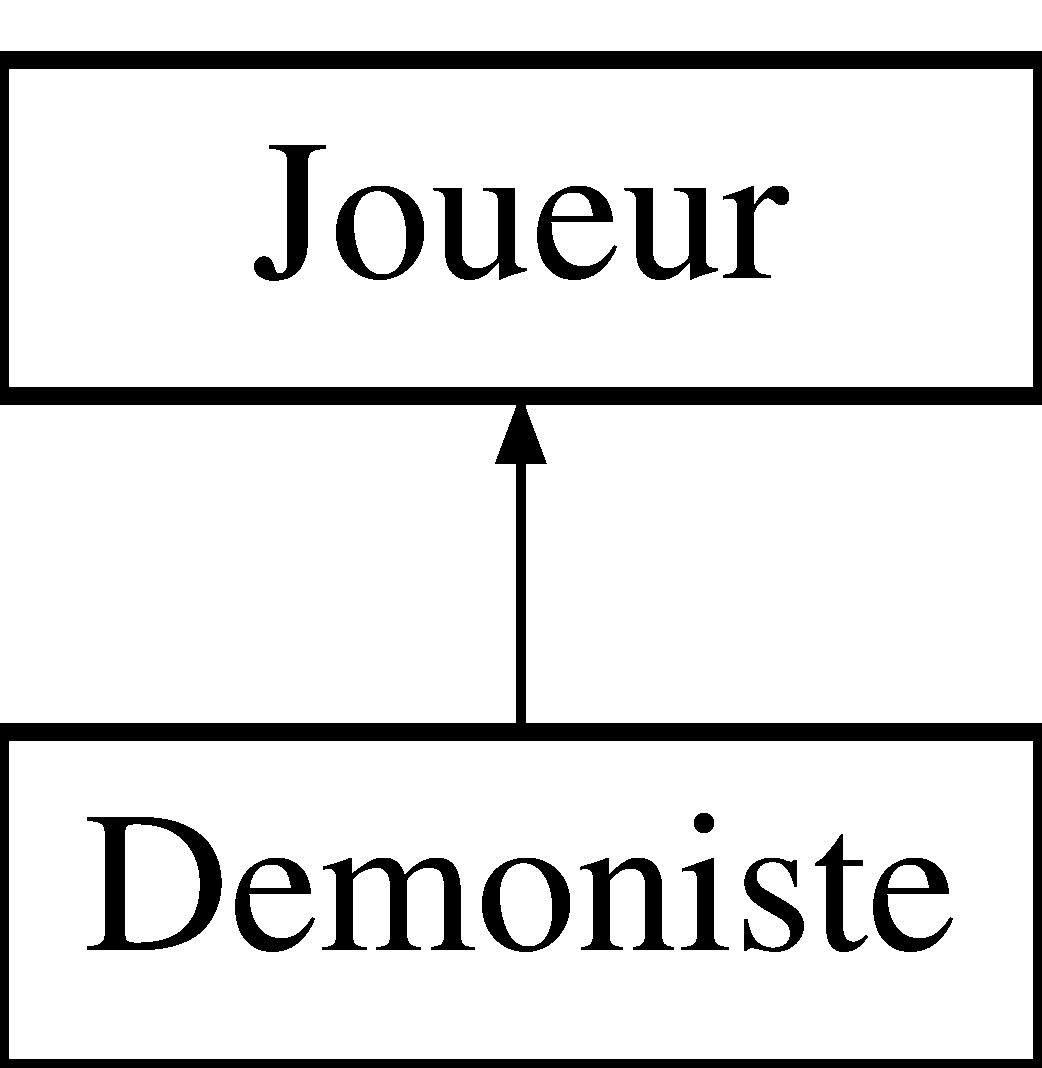
\includegraphics[height=2.000000cm]{class_demoniste}
\end{center}
\end{figure}
\subsection*{Fonctions membres publiques}
\begin{DoxyCompactItemize}
\item 
\hyperlink{class_demoniste_af380ca447e054e2096618ac7e2607c5a}{Demoniste} (std\-::string nom, std\-::string fichier)
\item 
\hyperlink{class_demoniste_ae66a10386b9ec772fe4b3d9e94deffe8}{$\sim$\-Demoniste} ()
\end{DoxyCompactItemize}


\subsection{Documentation des constructeurs et destructeur}
\hypertarget{class_demoniste_af380ca447e054e2096618ac7e2607c5a}{\index{Demoniste@{Demoniste}!Demoniste@{Demoniste}}
\index{Demoniste@{Demoniste}!Demoniste@{Demoniste}}
\subsubsection[{Demoniste}]{\setlength{\rightskip}{0pt plus 5cm}Demoniste\-::\-Demoniste (
\begin{DoxyParamCaption}
\item[{std\-::string}]{nom, }
\item[{std\-::string}]{fichier}
\end{DoxyParamCaption}
)}}\label{class_demoniste_af380ca447e054e2096618ac7e2607c5a}
Constructeur qui associe au \hyperlink{class_demoniste}{Demoniste} le comportement du pouvoir du \hyperlink{class_demoniste}{Demoniste} \hypertarget{class_demoniste_ae66a10386b9ec772fe4b3d9e94deffe8}{\index{Demoniste@{Demoniste}!$\sim$\-Demoniste@{$\sim$\-Demoniste}}
\index{$\sim$\-Demoniste@{$\sim$\-Demoniste}!Demoniste@{Demoniste}}
\subsubsection[{$\sim$\-Demoniste}]{\setlength{\rightskip}{0pt plus 5cm}Demoniste\-::$\sim$\-Demoniste (
\begin{DoxyParamCaption}
{}
\end{DoxyParamCaption}
)}}\label{class_demoniste_ae66a10386b9ec772fe4b3d9e94deffe8}
Destructeur 

La documentation de cette classe a été générée à partir des fichiers suivants \-:\begin{DoxyCompactItemize}
\item 
include/\-Modele/\-Joueur/\hyperlink{_demoniste_8hpp}{Demoniste.\-hpp}\item 
src/\-Modele/\-Joueur/\hyperlink{_demoniste_8cpp}{Demoniste.\-cpp}\end{DoxyCompactItemize}

\hypertarget{class_etat}{\section{Référence de la classe Etat}
\label{class_etat}\index{Etat@{Etat}}
}


{\ttfamily \#include $<$Etat.\-hpp$>$}

Graphe d'héritage de Etat\-:\begin{figure}[H]
\begin{center}
\leavevmode
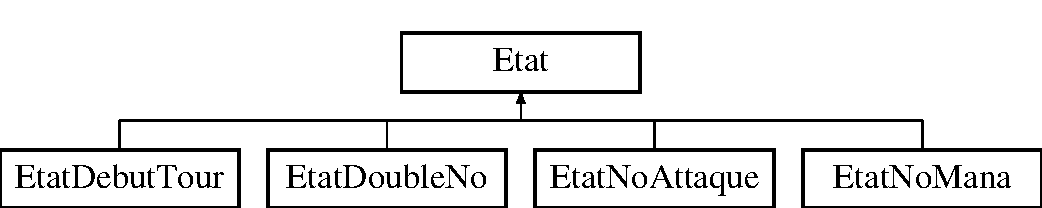
\includegraphics[height=2.000000cm]{class_etat}
\end{center}
\end{figure}
\subsection*{Fonctions membres publiques}
\begin{DoxyCompactItemize}
\item 
virtual \hyperlink{class_etat_a00bde3e769da5523e194a780ca95f7f7}{$\sim$\-Etat} ()
\item 
virtual void \hyperlink{class_etat_a41a3505b7477318292582ae544e7e0dd}{fin\-Tour} ()=0
\item 
virtual int \hyperlink{class_etat_ad76848f13da0e8e7f690a745e3075ab2}{afficher\-Choix\-Etat} ()=0
\end{DoxyCompactItemize}


\subsection{Description détaillée}
Fichier \hyperlink{_etat_8hpp}{Etat.\-hpp} \begin{DoxyAuthor}{Auteur}
Pierre Gaultier \& Theo Dolez 
\end{DoxyAuthor}


\subsection{Documentation des constructeurs et destructeur}
\hypertarget{class_etat_a00bde3e769da5523e194a780ca95f7f7}{\index{Etat@{Etat}!$\sim$\-Etat@{$\sim$\-Etat}}
\index{$\sim$\-Etat@{$\sim$\-Etat}!Etat@{Etat}}
\subsubsection[{$\sim$\-Etat}]{\setlength{\rightskip}{0pt plus 5cm}virtual Etat\-::$\sim$\-Etat (
\begin{DoxyParamCaption}
{}
\end{DoxyParamCaption}
)\hspace{0.3cm}{\ttfamily [inline]}, {\ttfamily [virtual]}}}\label{class_etat_a00bde3e769da5523e194a780ca95f7f7}


\subsection{Documentation des fonctions membres}
\hypertarget{class_etat_ad76848f13da0e8e7f690a745e3075ab2}{\index{Etat@{Etat}!afficher\-Choix\-Etat@{afficher\-Choix\-Etat}}
\index{afficher\-Choix\-Etat@{afficher\-Choix\-Etat}!Etat@{Etat}}
\subsubsection[{afficher\-Choix\-Etat}]{\setlength{\rightskip}{0pt plus 5cm}virtual int Etat\-::afficher\-Choix\-Etat (
\begin{DoxyParamCaption}
{}
\end{DoxyParamCaption}
)\hspace{0.3cm}{\ttfamily [pure virtual]}}}\label{class_etat_ad76848f13da0e8e7f690a745e3075ab2}


Implémenté dans \hyperlink{class_etat_debut_tour_a603db223f7f5f4c76fd6b978b54f33ae}{Etat\-Debut\-Tour}, \hyperlink{class_etat_double_no_a01af5700d0b3bd927af0d65f95395256}{Etat\-Double\-No}, \hyperlink{class_etat_no_attaque_ac89ab0d1f4483c7623617299b08922e3}{Etat\-No\-Attaque}, et \hyperlink{class_etat_no_mana_aa67bb9f558eaef0d07939a4747d12192}{Etat\-No\-Mana}.

\hypertarget{class_etat_a41a3505b7477318292582ae544e7e0dd}{\index{Etat@{Etat}!fin\-Tour@{fin\-Tour}}
\index{fin\-Tour@{fin\-Tour}!Etat@{Etat}}
\subsubsection[{fin\-Tour}]{\setlength{\rightskip}{0pt plus 5cm}virtual void Etat\-::fin\-Tour (
\begin{DoxyParamCaption}
{}
\end{DoxyParamCaption}
)\hspace{0.3cm}{\ttfamily [pure virtual]}}}\label{class_etat_a41a3505b7477318292582ae544e7e0dd}


Implémenté dans \hyperlink{class_etat_debut_tour_a0929f3701b5a1cda1e86aed3d2b40542}{Etat\-Debut\-Tour}, \hyperlink{class_etat_double_no_a888b25f87b975d3d92bfaa2cf9ce064d}{Etat\-Double\-No}, \hyperlink{class_etat_no_attaque_aea58b2b3580f3adbd93a4fa69398b51e}{Etat\-No\-Attaque}, et \hyperlink{class_etat_no_mana_a14567fee07c6c1a541885fcf2499cd56}{Etat\-No\-Mana}.



La documentation de cette classe a été générée à partir du fichier suivant \-:\begin{DoxyCompactItemize}
\item 
include/\-Controleur/\hyperlink{_etat_8hpp}{Etat.\-hpp}\end{DoxyCompactItemize}

\hypertarget{class_etat_debut_tour}{\section{Référence de la classe Etat\-Debut\-Tour}
\label{class_etat_debut_tour}\index{Etat\-Debut\-Tour@{Etat\-Debut\-Tour}}
}


{\ttfamily \#include $<$Etat\-Debut\-Tour.\-hpp$>$}

Graphe d'héritage de Etat\-Debut\-Tour\-:\begin{figure}[H]
\begin{center}
\leavevmode
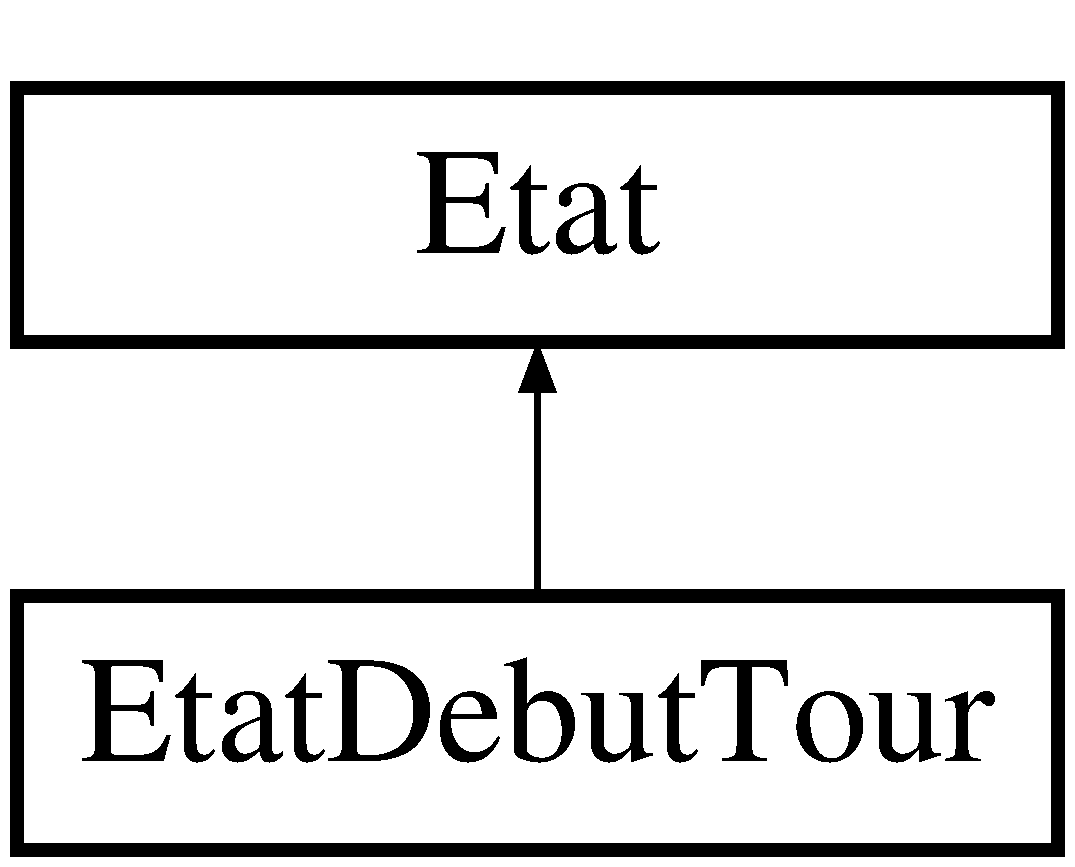
\includegraphics[height=2.000000cm]{class_etat_debut_tour}
\end{center}
\end{figure}
\subsection*{Fonctions membres publiques}
\begin{DoxyCompactItemize}
\item 
\hyperlink{class_etat_debut_tour_aa5b6ac2f696939c38ef726489c518975}{Etat\-Debut\-Tour} (\hyperlink{class_jeu}{Jeu} $\ast$j)
\item 
\hyperlink{class_etat_debut_tour_a615b6f4808730d92f52d9d1aa93a706d}{$\sim$\-Etat\-Debut\-Tour} ()
\item 
\hyperlink{class_jeu}{Jeu} $\ast$ \hyperlink{class_etat_debut_tour_a764bfcd224a4f306682d352a74f4cea8}{get\-Jeu} ()
\item 
int \hyperlink{class_etat_debut_tour_a603db223f7f5f4c76fd6b978b54f33ae}{afficher\-Choix\-Etat} ()
\item 
void \hyperlink{class_etat_debut_tour_a0929f3701b5a1cda1e86aed3d2b40542}{fin\-Tour} ()
\end{DoxyCompactItemize}
\subsection*{Attributs protégés}
\begin{DoxyCompactItemize}
\item 
\hyperlink{class_jeu}{Jeu} $\ast$ \hyperlink{class_etat_debut_tour_a0a54a446667e7868dc4a88efff67055d}{jeu}
\end{DoxyCompactItemize}


\subsection{Documentation des constructeurs et destructeur}
\hypertarget{class_etat_debut_tour_aa5b6ac2f696939c38ef726489c518975}{\index{Etat\-Debut\-Tour@{Etat\-Debut\-Tour}!Etat\-Debut\-Tour@{Etat\-Debut\-Tour}}
\index{Etat\-Debut\-Tour@{Etat\-Debut\-Tour}!EtatDebutTour@{Etat\-Debut\-Tour}}
\subsubsection[{Etat\-Debut\-Tour}]{\setlength{\rightskip}{0pt plus 5cm}Etat\-Debut\-Tour\-::\-Etat\-Debut\-Tour (
\begin{DoxyParamCaption}
\item[{{\bf Jeu} $\ast$}]{j}
\end{DoxyParamCaption}
)}}\label{class_etat_debut_tour_aa5b6ac2f696939c38ef726489c518975}
Constructeur. 
\begin{DoxyParams}{Paramètres}
{\em j} & le jeu \\
\hline
\end{DoxyParams}
\hypertarget{class_etat_debut_tour_a615b6f4808730d92f52d9d1aa93a706d}{\index{Etat\-Debut\-Tour@{Etat\-Debut\-Tour}!$\sim$\-Etat\-Debut\-Tour@{$\sim$\-Etat\-Debut\-Tour}}
\index{$\sim$\-Etat\-Debut\-Tour@{$\sim$\-Etat\-Debut\-Tour}!EtatDebutTour@{Etat\-Debut\-Tour}}
\subsubsection[{$\sim$\-Etat\-Debut\-Tour}]{\setlength{\rightskip}{0pt plus 5cm}Etat\-Debut\-Tour\-::$\sim$\-Etat\-Debut\-Tour (
\begin{DoxyParamCaption}
{}
\end{DoxyParamCaption}
)}}\label{class_etat_debut_tour_a615b6f4808730d92f52d9d1aa93a706d}
Destructeur 

\subsection{Documentation des fonctions membres}
\hypertarget{class_etat_debut_tour_a603db223f7f5f4c76fd6b978b54f33ae}{\index{Etat\-Debut\-Tour@{Etat\-Debut\-Tour}!afficher\-Choix\-Etat@{afficher\-Choix\-Etat}}
\index{afficher\-Choix\-Etat@{afficher\-Choix\-Etat}!EtatDebutTour@{Etat\-Debut\-Tour}}
\subsubsection[{afficher\-Choix\-Etat}]{\setlength{\rightskip}{0pt plus 5cm}int Etat\-Debut\-Tour\-::afficher\-Choix\-Etat (
\begin{DoxyParamCaption}
{}
\end{DoxyParamCaption}
)\hspace{0.3cm}{\ttfamily [virtual]}}}\label{class_etat_debut_tour_a603db223f7f5f4c76fd6b978b54f33ae}
Methode qui affiche les choix du \hyperlink{class_joueur}{Joueur} disponibles pour cet \hyperlink{class_etat}{Etat} et les exécute si le \hyperlink{class_joueur}{Joueur} entre les numéros associés. 

Implémente \hyperlink{class_etat_ad76848f13da0e8e7f690a745e3075ab2}{Etat}.

\hypertarget{class_etat_debut_tour_a0929f3701b5a1cda1e86aed3d2b40542}{\index{Etat\-Debut\-Tour@{Etat\-Debut\-Tour}!fin\-Tour@{fin\-Tour}}
\index{fin\-Tour@{fin\-Tour}!EtatDebutTour@{Etat\-Debut\-Tour}}
\subsubsection[{fin\-Tour}]{\setlength{\rightskip}{0pt plus 5cm}void Etat\-Debut\-Tour\-::fin\-Tour (
\begin{DoxyParamCaption}
{}
\end{DoxyParamCaption}
)\hspace{0.3cm}{\ttfamily [virtual]}}}\label{class_etat_debut_tour_a0929f3701b5a1cda1e86aed3d2b40542}
Methode qui termine le tour en cours, et lance le suivant 

Implémente \hyperlink{class_etat_a41a3505b7477318292582ae544e7e0dd}{Etat}.

\hypertarget{class_etat_debut_tour_a764bfcd224a4f306682d352a74f4cea8}{\index{Etat\-Debut\-Tour@{Etat\-Debut\-Tour}!get\-Jeu@{get\-Jeu}}
\index{get\-Jeu@{get\-Jeu}!EtatDebutTour@{Etat\-Debut\-Tour}}
\subsubsection[{get\-Jeu}]{\setlength{\rightskip}{0pt plus 5cm}{\bf Jeu} $\ast$ Etat\-Debut\-Tour\-::get\-Jeu (
\begin{DoxyParamCaption}
{}
\end{DoxyParamCaption}
)}}\label{class_etat_debut_tour_a764bfcd224a4f306682d352a74f4cea8}
Methode qui renvoie le jeu \begin{DoxyReturn}{Renvoie}
jeu le jeu 
\end{DoxyReturn}


\subsection{Documentation des données membres}
\hypertarget{class_etat_debut_tour_a0a54a446667e7868dc4a88efff67055d}{\index{Etat\-Debut\-Tour@{Etat\-Debut\-Tour}!jeu@{jeu}}
\index{jeu@{jeu}!EtatDebutTour@{Etat\-Debut\-Tour}}
\subsubsection[{jeu}]{\setlength{\rightskip}{0pt plus 5cm}{\bf Jeu}$\ast$ Etat\-Debut\-Tour\-::jeu\hspace{0.3cm}{\ttfamily [protected]}}}\label{class_etat_debut_tour_a0a54a446667e7868dc4a88efff67055d}


La documentation de cette classe a été générée à partir des fichiers suivants \-:\begin{DoxyCompactItemize}
\item 
include/\-Controleur/\hyperlink{_etat_debut_tour_8hpp}{Etat\-Debut\-Tour.\-hpp}\item 
src/\-Controleur/\hyperlink{_etat_debut_tour_8cpp}{Etat\-Debut\-Tour.\-cpp}\end{DoxyCompactItemize}

\hypertarget{class_etat_double_no}{\section{Référence de la classe Etat\-Double\-No}
\label{class_etat_double_no}\index{Etat\-Double\-No@{Etat\-Double\-No}}
}


{\ttfamily \#include $<$Etat\-Double\-No.\-hpp$>$}

Graphe d'héritage de Etat\-Double\-No\-:\begin{figure}[H]
\begin{center}
\leavevmode
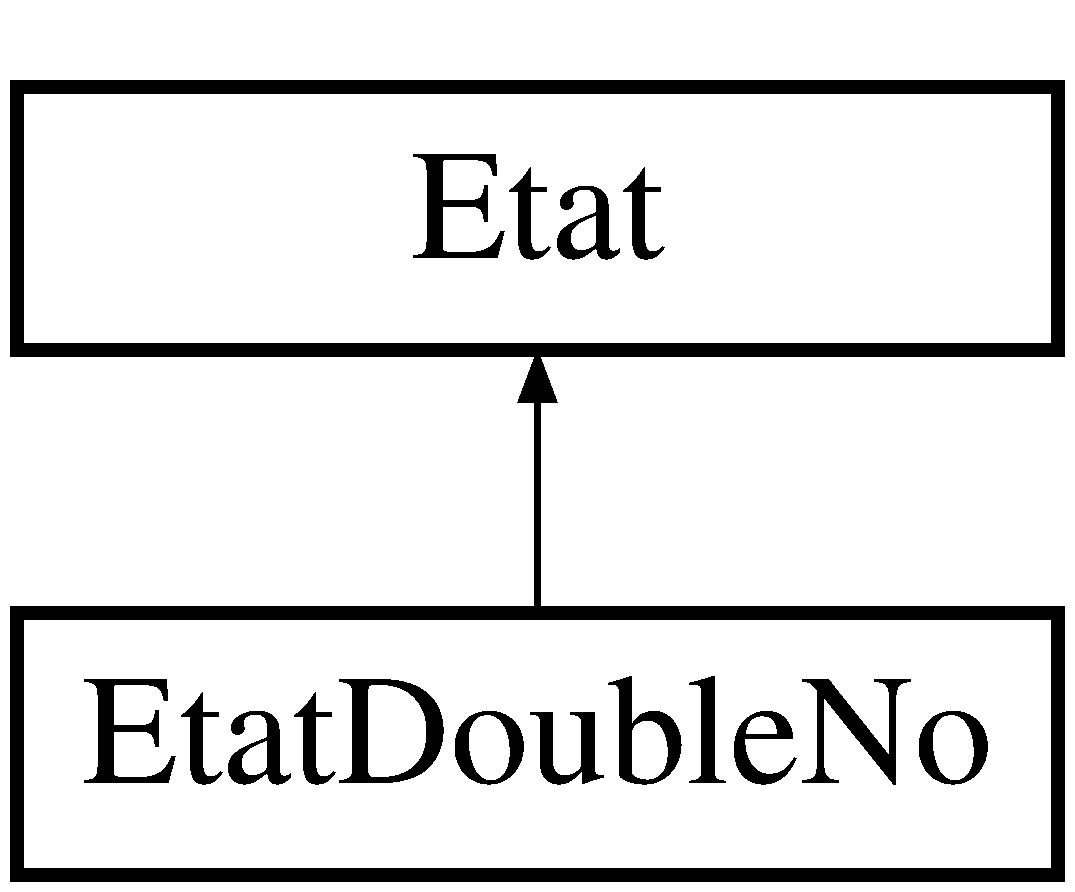
\includegraphics[height=2.000000cm]{class_etat_double_no}
\end{center}
\end{figure}
\subsection*{Fonctions membres publiques}
\begin{DoxyCompactItemize}
\item 
\hyperlink{class_etat_double_no_ac89c20bba357b6fff0d3d8aeead6b894}{Etat\-Double\-No} (\hyperlink{class_jeu}{Jeu} $\ast$j)
\item 
\hyperlink{class_etat_double_no_a5833701f2f11e8902ceb31626076dd2e}{$\sim$\-Etat\-Double\-No} ()
\item 
\hyperlink{class_jeu}{Jeu} $\ast$ \hyperlink{class_etat_double_no_a51f05fabae25436634e3b8c1ecdf5aef}{get\-Jeu} ()
\item 
int \hyperlink{class_etat_double_no_a01af5700d0b3bd927af0d65f95395256}{afficher\-Choix\-Etat} ()
\item 
void \hyperlink{class_etat_double_no_a888b25f87b975d3d92bfaa2cf9ce064d}{fin\-Tour} ()
\end{DoxyCompactItemize}
\subsection*{Attributs protégés}
\begin{DoxyCompactItemize}
\item 
\hyperlink{class_jeu}{Jeu} $\ast$ \hyperlink{class_etat_double_no_ac1166f725800d6a7f9c0c83bf6d7665e}{jeu}
\end{DoxyCompactItemize}


\subsection{Documentation des constructeurs et destructeur}
\hypertarget{class_etat_double_no_ac89c20bba357b6fff0d3d8aeead6b894}{\index{Etat\-Double\-No@{Etat\-Double\-No}!Etat\-Double\-No@{Etat\-Double\-No}}
\index{Etat\-Double\-No@{Etat\-Double\-No}!EtatDoubleNo@{Etat\-Double\-No}}
\subsubsection[{Etat\-Double\-No}]{\setlength{\rightskip}{0pt plus 5cm}Etat\-Double\-No\-::\-Etat\-Double\-No (
\begin{DoxyParamCaption}
\item[{{\bf Jeu} $\ast$}]{j}
\end{DoxyParamCaption}
)}}\label{class_etat_double_no_ac89c20bba357b6fff0d3d8aeead6b894}
Constructeur. 
\begin{DoxyParams}{Paramètres}
{\em j} & le jeu \\
\hline
\end{DoxyParams}
\hypertarget{class_etat_double_no_a5833701f2f11e8902ceb31626076dd2e}{\index{Etat\-Double\-No@{Etat\-Double\-No}!$\sim$\-Etat\-Double\-No@{$\sim$\-Etat\-Double\-No}}
\index{$\sim$\-Etat\-Double\-No@{$\sim$\-Etat\-Double\-No}!EtatDoubleNo@{Etat\-Double\-No}}
\subsubsection[{$\sim$\-Etat\-Double\-No}]{\setlength{\rightskip}{0pt plus 5cm}Etat\-Double\-No\-::$\sim$\-Etat\-Double\-No (
\begin{DoxyParamCaption}
{}
\end{DoxyParamCaption}
)}}\label{class_etat_double_no_a5833701f2f11e8902ceb31626076dd2e}
Destructeur 

\subsection{Documentation des fonctions membres}
\hypertarget{class_etat_double_no_a01af5700d0b3bd927af0d65f95395256}{\index{Etat\-Double\-No@{Etat\-Double\-No}!afficher\-Choix\-Etat@{afficher\-Choix\-Etat}}
\index{afficher\-Choix\-Etat@{afficher\-Choix\-Etat}!EtatDoubleNo@{Etat\-Double\-No}}
\subsubsection[{afficher\-Choix\-Etat}]{\setlength{\rightskip}{0pt plus 5cm}int Etat\-Double\-No\-::afficher\-Choix\-Etat (
\begin{DoxyParamCaption}
{}
\end{DoxyParamCaption}
)\hspace{0.3cm}{\ttfamily [virtual]}}}\label{class_etat_double_no_a01af5700d0b3bd927af0d65f95395256}
Methode qui affiche les choix du \hyperlink{class_joueur}{Joueur} disponibles pour cet \hyperlink{class_etat}{Etat} et les exécute si le \hyperlink{class_joueur}{Joueur} entre les numéros associés. 

Implémente \hyperlink{class_etat_ad76848f13da0e8e7f690a745e3075ab2}{Etat}.

\hypertarget{class_etat_double_no_a888b25f87b975d3d92bfaa2cf9ce064d}{\index{Etat\-Double\-No@{Etat\-Double\-No}!fin\-Tour@{fin\-Tour}}
\index{fin\-Tour@{fin\-Tour}!EtatDoubleNo@{Etat\-Double\-No}}
\subsubsection[{fin\-Tour}]{\setlength{\rightskip}{0pt plus 5cm}void Etat\-Double\-No\-::fin\-Tour (
\begin{DoxyParamCaption}
{}
\end{DoxyParamCaption}
)\hspace{0.3cm}{\ttfamily [virtual]}}}\label{class_etat_double_no_a888b25f87b975d3d92bfaa2cf9ce064d}
Methode qui termine le tour en cours, et lance le suivant 

Implémente \hyperlink{class_etat_a41a3505b7477318292582ae544e7e0dd}{Etat}.

\hypertarget{class_etat_double_no_a51f05fabae25436634e3b8c1ecdf5aef}{\index{Etat\-Double\-No@{Etat\-Double\-No}!get\-Jeu@{get\-Jeu}}
\index{get\-Jeu@{get\-Jeu}!EtatDoubleNo@{Etat\-Double\-No}}
\subsubsection[{get\-Jeu}]{\setlength{\rightskip}{0pt plus 5cm}{\bf Jeu} $\ast$ Etat\-Double\-No\-::get\-Jeu (
\begin{DoxyParamCaption}
{}
\end{DoxyParamCaption}
)}}\label{class_etat_double_no_a51f05fabae25436634e3b8c1ecdf5aef}
Methode qui renvoie le jeu \begin{DoxyReturn}{Renvoie}
jeu le jeu 
\end{DoxyReturn}


\subsection{Documentation des données membres}
\hypertarget{class_etat_double_no_ac1166f725800d6a7f9c0c83bf6d7665e}{\index{Etat\-Double\-No@{Etat\-Double\-No}!jeu@{jeu}}
\index{jeu@{jeu}!EtatDoubleNo@{Etat\-Double\-No}}
\subsubsection[{jeu}]{\setlength{\rightskip}{0pt plus 5cm}{\bf Jeu}$\ast$ Etat\-Double\-No\-::jeu\hspace{0.3cm}{\ttfamily [protected]}}}\label{class_etat_double_no_ac1166f725800d6a7f9c0c83bf6d7665e}


La documentation de cette classe a été générée à partir des fichiers suivants \-:\begin{DoxyCompactItemize}
\item 
include/\-Controleur/\hyperlink{_etat_double_no_8hpp}{Etat\-Double\-No.\-hpp}\item 
src/\-Controleur/\hyperlink{_etat_double_no_8cpp}{Etat\-Double\-No.\-cpp}\end{DoxyCompactItemize}

\hypertarget{class_etat_no_attaque}{\section{Référence de la classe Etat\-No\-Attaque}
\label{class_etat_no_attaque}\index{Etat\-No\-Attaque@{Etat\-No\-Attaque}}
}


{\ttfamily \#include $<$Etat\-No\-Attaque.\-hpp$>$}

Graphe d'héritage de Etat\-No\-Attaque\-:\begin{figure}[H]
\begin{center}
\leavevmode
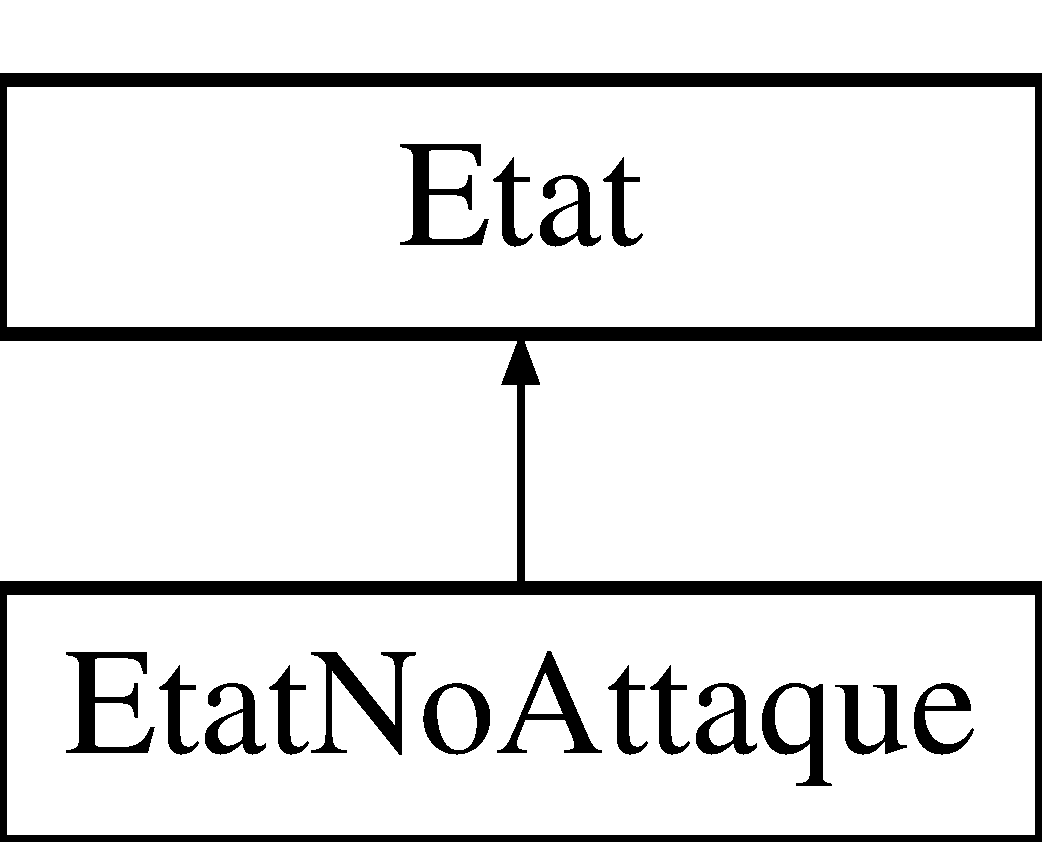
\includegraphics[height=2.000000cm]{class_etat_no_attaque}
\end{center}
\end{figure}
\subsection*{Fonctions membres publiques}
\begin{DoxyCompactItemize}
\item 
\hyperlink{class_etat_no_attaque_a39b37880a28e5cbda92e584221b9a68d}{Etat\-No\-Attaque} (\hyperlink{class_jeu}{Jeu} $\ast$j)
\item 
\hyperlink{class_etat_no_attaque_a81a0114551961e5780e7e3866f22c6fb}{$\sim$\-Etat\-No\-Attaque} ()
\item 
\hyperlink{class_jeu}{Jeu} $\ast$ \hyperlink{class_etat_no_attaque_ab98d57f8da5876194e0c1496f137c613}{get\-Jeu} ()
\item 
int \hyperlink{class_etat_no_attaque_ac89ab0d1f4483c7623617299b08922e3}{afficher\-Choix\-Etat} ()
\item 
void \hyperlink{class_etat_no_attaque_aea58b2b3580f3adbd93a4fa69398b51e}{fin\-Tour} ()
\end{DoxyCompactItemize}
\subsection*{Attributs protégés}
\begin{DoxyCompactItemize}
\item 
\hyperlink{class_jeu}{Jeu} $\ast$ \hyperlink{class_etat_no_attaque_ad5dbee65b31bd41e28a648ac22bbbfce}{jeu}
\end{DoxyCompactItemize}


\subsection{Documentation des constructeurs et destructeur}
\hypertarget{class_etat_no_attaque_a39b37880a28e5cbda92e584221b9a68d}{\index{Etat\-No\-Attaque@{Etat\-No\-Attaque}!Etat\-No\-Attaque@{Etat\-No\-Attaque}}
\index{Etat\-No\-Attaque@{Etat\-No\-Attaque}!EtatNoAttaque@{Etat\-No\-Attaque}}
\subsubsection[{Etat\-No\-Attaque}]{\setlength{\rightskip}{0pt plus 5cm}Etat\-No\-Attaque\-::\-Etat\-No\-Attaque (
\begin{DoxyParamCaption}
\item[{{\bf Jeu} $\ast$}]{j}
\end{DoxyParamCaption}
)}}\label{class_etat_no_attaque_a39b37880a28e5cbda92e584221b9a68d}
Constructeur. 
\begin{DoxyParams}{Paramètres}
{\em j} & le jeu \\
\hline
\end{DoxyParams}
\hypertarget{class_etat_no_attaque_a81a0114551961e5780e7e3866f22c6fb}{\index{Etat\-No\-Attaque@{Etat\-No\-Attaque}!$\sim$\-Etat\-No\-Attaque@{$\sim$\-Etat\-No\-Attaque}}
\index{$\sim$\-Etat\-No\-Attaque@{$\sim$\-Etat\-No\-Attaque}!EtatNoAttaque@{Etat\-No\-Attaque}}
\subsubsection[{$\sim$\-Etat\-No\-Attaque}]{\setlength{\rightskip}{0pt plus 5cm}Etat\-No\-Attaque\-::$\sim$\-Etat\-No\-Attaque (
\begin{DoxyParamCaption}
{}
\end{DoxyParamCaption}
)}}\label{class_etat_no_attaque_a81a0114551961e5780e7e3866f22c6fb}
Destructeur 

\subsection{Documentation des fonctions membres}
\hypertarget{class_etat_no_attaque_ac89ab0d1f4483c7623617299b08922e3}{\index{Etat\-No\-Attaque@{Etat\-No\-Attaque}!afficher\-Choix\-Etat@{afficher\-Choix\-Etat}}
\index{afficher\-Choix\-Etat@{afficher\-Choix\-Etat}!EtatNoAttaque@{Etat\-No\-Attaque}}
\subsubsection[{afficher\-Choix\-Etat}]{\setlength{\rightskip}{0pt plus 5cm}int Etat\-No\-Attaque\-::afficher\-Choix\-Etat (
\begin{DoxyParamCaption}
{}
\end{DoxyParamCaption}
)\hspace{0.3cm}{\ttfamily [virtual]}}}\label{class_etat_no_attaque_ac89ab0d1f4483c7623617299b08922e3}
Methode qui affiche les choix du \hyperlink{class_joueur}{Joueur} disponibles pour cet \hyperlink{class_etat}{Etat} et les exécute si le \hyperlink{class_joueur}{Joueur} entre les numéros associés. 

Implémente \hyperlink{class_etat_ad76848f13da0e8e7f690a745e3075ab2}{Etat}.

\hypertarget{class_etat_no_attaque_aea58b2b3580f3adbd93a4fa69398b51e}{\index{Etat\-No\-Attaque@{Etat\-No\-Attaque}!fin\-Tour@{fin\-Tour}}
\index{fin\-Tour@{fin\-Tour}!EtatNoAttaque@{Etat\-No\-Attaque}}
\subsubsection[{fin\-Tour}]{\setlength{\rightskip}{0pt plus 5cm}void Etat\-No\-Attaque\-::fin\-Tour (
\begin{DoxyParamCaption}
{}
\end{DoxyParamCaption}
)\hspace{0.3cm}{\ttfamily [virtual]}}}\label{class_etat_no_attaque_aea58b2b3580f3adbd93a4fa69398b51e}
Methode qui termine le tour en cours, et lance le suivant 

Implémente \hyperlink{class_etat_a41a3505b7477318292582ae544e7e0dd}{Etat}.

\hypertarget{class_etat_no_attaque_ab98d57f8da5876194e0c1496f137c613}{\index{Etat\-No\-Attaque@{Etat\-No\-Attaque}!get\-Jeu@{get\-Jeu}}
\index{get\-Jeu@{get\-Jeu}!EtatNoAttaque@{Etat\-No\-Attaque}}
\subsubsection[{get\-Jeu}]{\setlength{\rightskip}{0pt plus 5cm}{\bf Jeu} $\ast$ Etat\-No\-Attaque\-::get\-Jeu (
\begin{DoxyParamCaption}
{}
\end{DoxyParamCaption}
)}}\label{class_etat_no_attaque_ab98d57f8da5876194e0c1496f137c613}
Methode qui renvoie le jeu \begin{DoxyReturn}{Renvoie}
jeu le jeu 
\end{DoxyReturn}


\subsection{Documentation des données membres}
\hypertarget{class_etat_no_attaque_ad5dbee65b31bd41e28a648ac22bbbfce}{\index{Etat\-No\-Attaque@{Etat\-No\-Attaque}!jeu@{jeu}}
\index{jeu@{jeu}!EtatNoAttaque@{Etat\-No\-Attaque}}
\subsubsection[{jeu}]{\setlength{\rightskip}{0pt plus 5cm}{\bf Jeu}$\ast$ Etat\-No\-Attaque\-::jeu\hspace{0.3cm}{\ttfamily [protected]}}}\label{class_etat_no_attaque_ad5dbee65b31bd41e28a648ac22bbbfce}


La documentation de cette classe a été générée à partir des fichiers suivants \-:\begin{DoxyCompactItemize}
\item 
include/\-Controleur/\hyperlink{_etat_no_attaque_8hpp}{Etat\-No\-Attaque.\-hpp}\item 
src/\-Controleur/\hyperlink{_etat_no_attaque_8cpp}{Etat\-No\-Attaque.\-cpp}\end{DoxyCompactItemize}

\hypertarget{class_etat_no_mana}{\section{Référence de la classe Etat\-No\-Mana}
\label{class_etat_no_mana}\index{Etat\-No\-Mana@{Etat\-No\-Mana}}
}


{\ttfamily \#include $<$Etat\-No\-Mana.\-hpp$>$}

Graphe d'héritage de Etat\-No\-Mana\-:\begin{figure}[H]
\begin{center}
\leavevmode
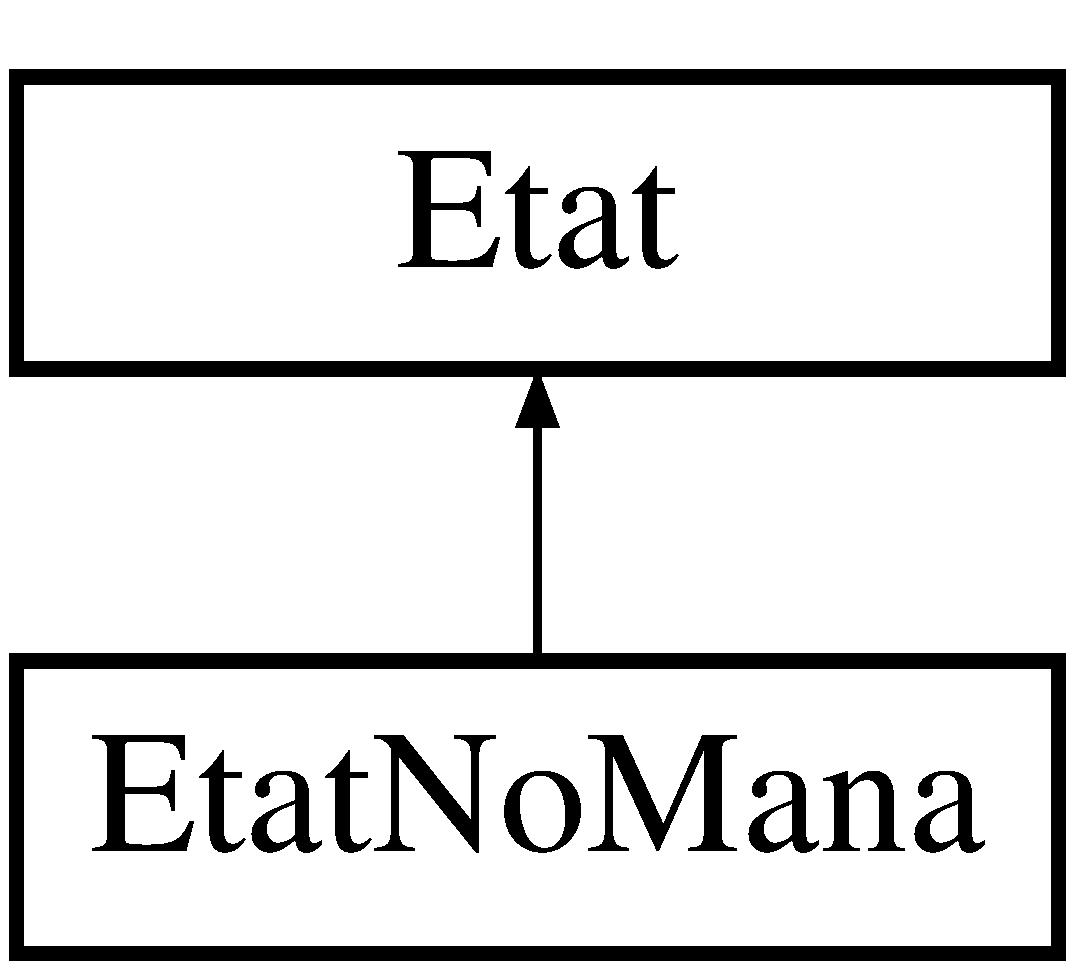
\includegraphics[height=2.000000cm]{class_etat_no_mana}
\end{center}
\end{figure}
\subsection*{Fonctions membres publiques}
\begin{DoxyCompactItemize}
\item 
\hyperlink{class_etat_no_mana_a506d5de276476b23f9c86864b4c439fa}{Etat\-No\-Mana} (\hyperlink{class_jeu}{Jeu} $\ast$j)
\item 
\hyperlink{class_etat_no_mana_aaae2ecdedcef4451b0a0f7c88aad4c71}{$\sim$\-Etat\-No\-Mana} ()
\item 
\hyperlink{class_jeu}{Jeu} $\ast$ \hyperlink{class_etat_no_mana_a153d0656498f8e15d0c550fc4898f5fe}{get\-Jeu} ()
\item 
int \hyperlink{class_etat_no_mana_aa67bb9f558eaef0d07939a4747d12192}{afficher\-Choix\-Etat} ()
\item 
void \hyperlink{class_etat_no_mana_a14567fee07c6c1a541885fcf2499cd56}{fin\-Tour} ()
\end{DoxyCompactItemize}
\subsection*{Attributs protégés}
\begin{DoxyCompactItemize}
\item 
\hyperlink{class_jeu}{Jeu} $\ast$ \hyperlink{class_etat_no_mana_a8ddcdb9981a36c8baa31d1979272ff72}{jeu}
\end{DoxyCompactItemize}


\subsection{Documentation des constructeurs et destructeur}
\hypertarget{class_etat_no_mana_a506d5de276476b23f9c86864b4c439fa}{\index{Etat\-No\-Mana@{Etat\-No\-Mana}!Etat\-No\-Mana@{Etat\-No\-Mana}}
\index{Etat\-No\-Mana@{Etat\-No\-Mana}!EtatNoMana@{Etat\-No\-Mana}}
\subsubsection[{Etat\-No\-Mana}]{\setlength{\rightskip}{0pt plus 5cm}Etat\-No\-Mana\-::\-Etat\-No\-Mana (
\begin{DoxyParamCaption}
\item[{{\bf Jeu} $\ast$}]{j}
\end{DoxyParamCaption}
)}}\label{class_etat_no_mana_a506d5de276476b23f9c86864b4c439fa}
Constructeur. 
\begin{DoxyParams}{Paramètres}
{\em j} & le jeu \\
\hline
\end{DoxyParams}
\hypertarget{class_etat_no_mana_aaae2ecdedcef4451b0a0f7c88aad4c71}{\index{Etat\-No\-Mana@{Etat\-No\-Mana}!$\sim$\-Etat\-No\-Mana@{$\sim$\-Etat\-No\-Mana}}
\index{$\sim$\-Etat\-No\-Mana@{$\sim$\-Etat\-No\-Mana}!EtatNoMana@{Etat\-No\-Mana}}
\subsubsection[{$\sim$\-Etat\-No\-Mana}]{\setlength{\rightskip}{0pt plus 5cm}Etat\-No\-Mana\-::$\sim$\-Etat\-No\-Mana (
\begin{DoxyParamCaption}
{}
\end{DoxyParamCaption}
)}}\label{class_etat_no_mana_aaae2ecdedcef4451b0a0f7c88aad4c71}
Destructeur 

\subsection{Documentation des fonctions membres}
\hypertarget{class_etat_no_mana_aa67bb9f558eaef0d07939a4747d12192}{\index{Etat\-No\-Mana@{Etat\-No\-Mana}!afficher\-Choix\-Etat@{afficher\-Choix\-Etat}}
\index{afficher\-Choix\-Etat@{afficher\-Choix\-Etat}!EtatNoMana@{Etat\-No\-Mana}}
\subsubsection[{afficher\-Choix\-Etat}]{\setlength{\rightskip}{0pt plus 5cm}int Etat\-No\-Mana\-::afficher\-Choix\-Etat (
\begin{DoxyParamCaption}
{}
\end{DoxyParamCaption}
)\hspace{0.3cm}{\ttfamily [virtual]}}}\label{class_etat_no_mana_aa67bb9f558eaef0d07939a4747d12192}
Methode qui affiche les choix du \hyperlink{class_joueur}{Joueur} disponibles pour cet \hyperlink{class_etat}{Etat} et les exécute si le \hyperlink{class_joueur}{Joueur} entre les numéros associés. 

Implémente \hyperlink{class_etat_ad76848f13da0e8e7f690a745e3075ab2}{Etat}.

\hypertarget{class_etat_no_mana_a14567fee07c6c1a541885fcf2499cd56}{\index{Etat\-No\-Mana@{Etat\-No\-Mana}!fin\-Tour@{fin\-Tour}}
\index{fin\-Tour@{fin\-Tour}!EtatNoMana@{Etat\-No\-Mana}}
\subsubsection[{fin\-Tour}]{\setlength{\rightskip}{0pt plus 5cm}void Etat\-No\-Mana\-::fin\-Tour (
\begin{DoxyParamCaption}
{}
\end{DoxyParamCaption}
)\hspace{0.3cm}{\ttfamily [virtual]}}}\label{class_etat_no_mana_a14567fee07c6c1a541885fcf2499cd56}
Methode qui termine le tour en cours, et lance le suivant 

Implémente \hyperlink{class_etat_a41a3505b7477318292582ae544e7e0dd}{Etat}.

\hypertarget{class_etat_no_mana_a153d0656498f8e15d0c550fc4898f5fe}{\index{Etat\-No\-Mana@{Etat\-No\-Mana}!get\-Jeu@{get\-Jeu}}
\index{get\-Jeu@{get\-Jeu}!EtatNoMana@{Etat\-No\-Mana}}
\subsubsection[{get\-Jeu}]{\setlength{\rightskip}{0pt plus 5cm}{\bf Jeu} $\ast$ Etat\-No\-Mana\-::get\-Jeu (
\begin{DoxyParamCaption}
{}
\end{DoxyParamCaption}
)}}\label{class_etat_no_mana_a153d0656498f8e15d0c550fc4898f5fe}
Methode qui renvoie le jeu \begin{DoxyReturn}{Renvoie}
jeu le jeu 
\end{DoxyReturn}


\subsection{Documentation des données membres}
\hypertarget{class_etat_no_mana_a8ddcdb9981a36c8baa31d1979272ff72}{\index{Etat\-No\-Mana@{Etat\-No\-Mana}!jeu@{jeu}}
\index{jeu@{jeu}!EtatNoMana@{Etat\-No\-Mana}}
\subsubsection[{jeu}]{\setlength{\rightskip}{0pt plus 5cm}{\bf Jeu}$\ast$ Etat\-No\-Mana\-::jeu\hspace{0.3cm}{\ttfamily [protected]}}}\label{class_etat_no_mana_a8ddcdb9981a36c8baa31d1979272ff72}


La documentation de cette classe a été générée à partir des fichiers suivants \-:\begin{DoxyCompactItemize}
\item 
include/\-Controleur/\hyperlink{_etat_no_mana_8hpp}{Etat\-No\-Mana.\-hpp}\item 
src/\-Controleur/\hyperlink{_etat_no_mana_8cpp}{Etat\-No\-Mana.\-cpp}\end{DoxyCompactItemize}

\hypertarget{class_fin_de_jeu}{\section{Référence de la classe Fin\-De\-Jeu}
\label{class_fin_de_jeu}\index{Fin\-De\-Jeu@{Fin\-De\-Jeu}}
}


{\ttfamily \#include $<$Fin\-De\-Jeu.\-hpp$>$}

Graphe d'héritage de Fin\-De\-Jeu\-:\begin{figure}[H]
\begin{center}
\leavevmode
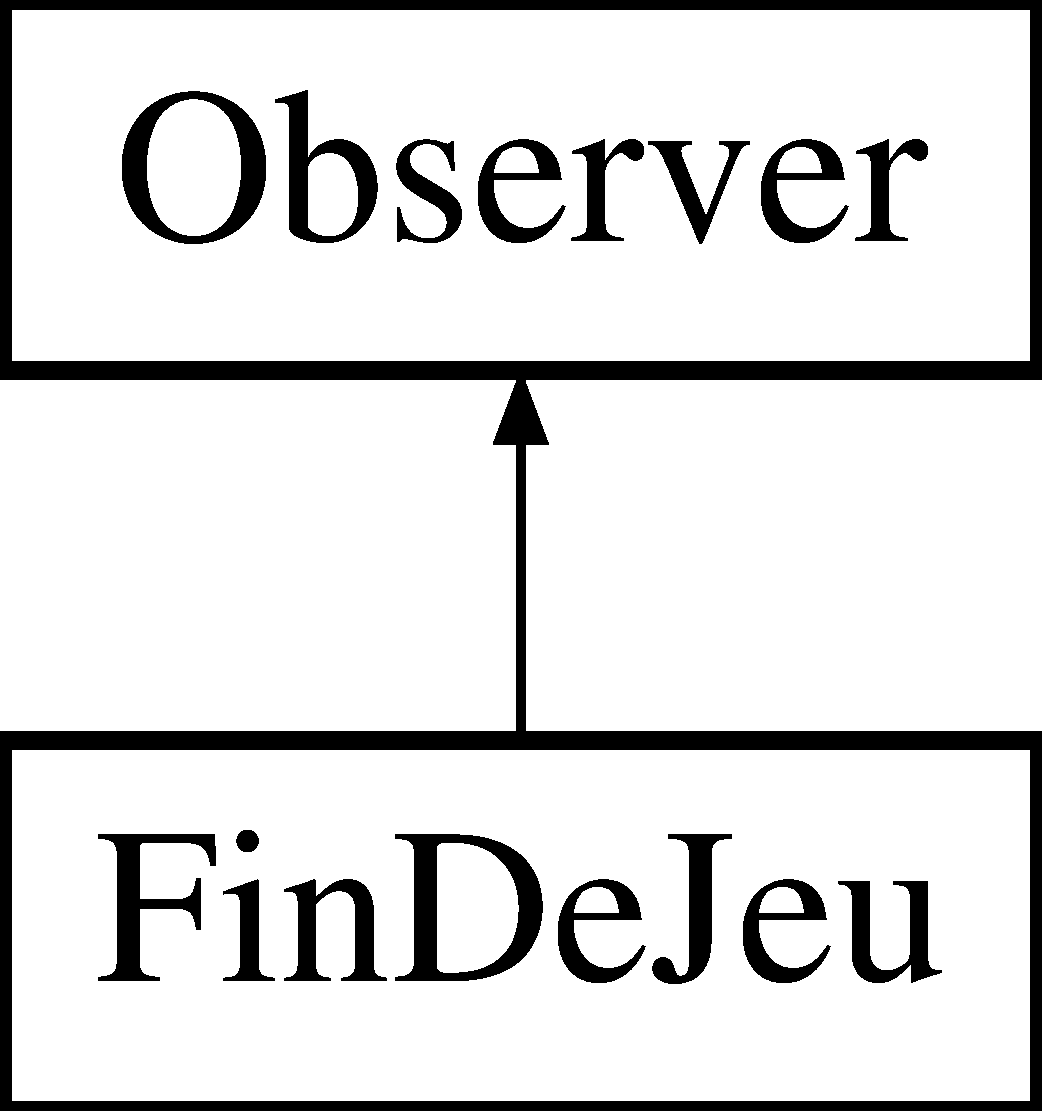
\includegraphics[height=2.000000cm]{class_fin_de_jeu}
\end{center}
\end{figure}
\subsection*{Fonctions membres publiques}
\begin{DoxyCompactItemize}
\item 
\hyperlink{class_fin_de_jeu_af86c4d468aec3ffb9ed59c02016aadcf}{Fin\-De\-Jeu} (\hyperlink{class_jeu}{Jeu} $\ast$j)
\item 
\hyperlink{class_fin_de_jeu_a7f80425c93ed96eadb13ac5e7bb51bd4}{$\sim$\-Fin\-De\-Jeu} ()
\item 
bool \hyperlink{class_fin_de_jeu_a79c3fb0a9e367cd3e62da14af840f871}{actualiser} ()
\end{DoxyCompactItemize}


\subsection{Description détaillée}
Fichier \hyperlink{_fin_de_jeu_8hpp}{Fin\-De\-Jeu.\-hpp} \begin{DoxyAuthor}{Auteur}
Pierre Gaultier \& Theo Dolez 
\end{DoxyAuthor}


\subsection{Documentation des constructeurs et destructeur}
\hypertarget{class_fin_de_jeu_af86c4d468aec3ffb9ed59c02016aadcf}{\index{Fin\-De\-Jeu@{Fin\-De\-Jeu}!Fin\-De\-Jeu@{Fin\-De\-Jeu}}
\index{Fin\-De\-Jeu@{Fin\-De\-Jeu}!FinDeJeu@{Fin\-De\-Jeu}}
\subsubsection[{Fin\-De\-Jeu}]{\setlength{\rightskip}{0pt plus 5cm}Fin\-De\-Jeu\-::\-Fin\-De\-Jeu (
\begin{DoxyParamCaption}
\item[{{\bf Jeu} $\ast$}]{j}
\end{DoxyParamCaption}
)}}\label{class_fin_de_jeu_af86c4d468aec3ffb9ed59c02016aadcf}
Constructeur 
\begin{DoxyParams}{Paramètres}
{\em s} & \hyperlink{class_sujet}{Sujet} de l'observer \\
\hline
\end{DoxyParams}
\hypertarget{class_fin_de_jeu_a7f80425c93ed96eadb13ac5e7bb51bd4}{\index{Fin\-De\-Jeu@{Fin\-De\-Jeu}!$\sim$\-Fin\-De\-Jeu@{$\sim$\-Fin\-De\-Jeu}}
\index{$\sim$\-Fin\-De\-Jeu@{$\sim$\-Fin\-De\-Jeu}!FinDeJeu@{Fin\-De\-Jeu}}
\subsubsection[{$\sim$\-Fin\-De\-Jeu}]{\setlength{\rightskip}{0pt plus 5cm}Fin\-De\-Jeu\-::$\sim$\-Fin\-De\-Jeu (
\begin{DoxyParamCaption}
{}
\end{DoxyParamCaption}
)}}\label{class_fin_de_jeu_a7f80425c93ed96eadb13ac5e7bb51bd4}
Destructeur 

\subsection{Documentation des fonctions membres}
\hypertarget{class_fin_de_jeu_a79c3fb0a9e367cd3e62da14af840f871}{\index{Fin\-De\-Jeu@{Fin\-De\-Jeu}!actualiser@{actualiser}}
\index{actualiser@{actualiser}!FinDeJeu@{Fin\-De\-Jeu}}
\subsubsection[{actualiser}]{\setlength{\rightskip}{0pt plus 5cm}bool Fin\-De\-Jeu\-::actualiser (
\begin{DoxyParamCaption}
{}
\end{DoxyParamCaption}
)\hspace{0.3cm}{\ttfamily [virtual]}}}\label{class_fin_de_jeu_a79c3fb0a9e367cd3e62da14af840f871}
Methode qui actualise le jeu \begin{DoxyReturn}{Renvoie}
Jeu\-Termine boolean. 
\end{DoxyReturn}


Implémente \hyperlink{class_observer_a7930233e1f70d67b3fece5d05e5b6299}{Observer}.



La documentation de cette classe a été générée à partir des fichiers suivants \-:\begin{DoxyCompactItemize}
\item 
include/\-Controleur/\hyperlink{_fin_de_jeu_8hpp}{Fin\-De\-Jeu.\-hpp}\item 
src/\-Controleur/\hyperlink{_fin_de_jeu_8cpp}{Fin\-De\-Jeu.\-cpp}\end{DoxyCompactItemize}

\hypertarget{class_guerrier}{\section{Référence de la classe Guerrier}
\label{class_guerrier}\index{Guerrier@{Guerrier}}
}


{\ttfamily \#include $<$Guerrier.\-hpp$>$}

Graphe d'héritage de Guerrier\-:\begin{figure}[H]
\begin{center}
\leavevmode
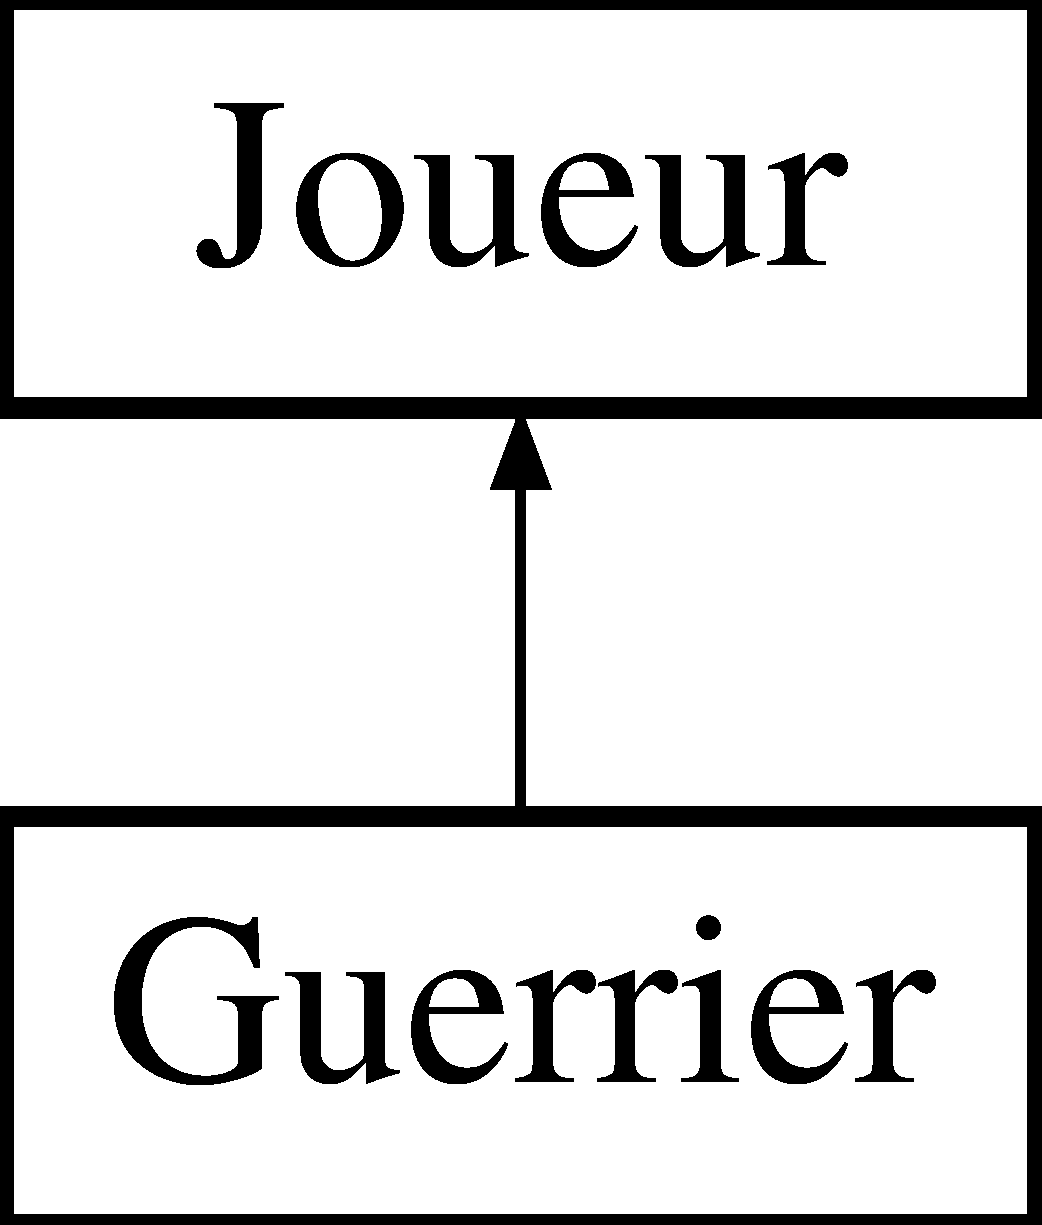
\includegraphics[height=2.000000cm]{class_guerrier}
\end{center}
\end{figure}
\subsection*{Fonctions membres publiques}
\begin{DoxyCompactItemize}
\item 
\hyperlink{class_guerrier_a08622f52e49c7fd2695ce215b3ad9aec}{Guerrier} (std\-::string nom, std\-::string fichier)
\item 
\hyperlink{class_guerrier_a83ec8ec6ced25a349249d0cdc70c75b6}{$\sim$\-Guerrier} ()
\end{DoxyCompactItemize}


\subsection{Description détaillée}
Fichier \hyperlink{_guerrier_8hpp}{Guerrier.\-hpp} \begin{DoxyAuthor}{Auteur}
Pierre Gaultier \& Theo Dolez 
\end{DoxyAuthor}


\subsection{Documentation des constructeurs et destructeur}
\hypertarget{class_guerrier_a08622f52e49c7fd2695ce215b3ad9aec}{\index{Guerrier@{Guerrier}!Guerrier@{Guerrier}}
\index{Guerrier@{Guerrier}!Guerrier@{Guerrier}}
\subsubsection[{Guerrier}]{\setlength{\rightskip}{0pt plus 5cm}Guerrier\-::\-Guerrier (
\begin{DoxyParamCaption}
\item[{std\-::string}]{nom, }
\item[{std\-::string}]{fichier}
\end{DoxyParamCaption}
)}}\label{class_guerrier_a08622f52e49c7fd2695ce215b3ad9aec}
Constructeur qui associe au \hyperlink{class_guerrier}{Guerrier} le comportement du pouvoir du \hyperlink{class_guerrier}{Guerrier} \hypertarget{class_guerrier_a83ec8ec6ced25a349249d0cdc70c75b6}{\index{Guerrier@{Guerrier}!$\sim$\-Guerrier@{$\sim$\-Guerrier}}
\index{$\sim$\-Guerrier@{$\sim$\-Guerrier}!Guerrier@{Guerrier}}
\subsubsection[{$\sim$\-Guerrier}]{\setlength{\rightskip}{0pt plus 5cm}Guerrier\-::$\sim$\-Guerrier (
\begin{DoxyParamCaption}
{}
\end{DoxyParamCaption}
)}}\label{class_guerrier_a83ec8ec6ced25a349249d0cdc70c75b6}
Destructeur 

La documentation de cette classe a été générée à partir des fichiers suivants \-:\begin{DoxyCompactItemize}
\item 
include/\-Modele/\-Joueur/\hyperlink{_guerrier_8hpp}{Guerrier.\-hpp}\item 
src/\-Modele/\-Joueur/\hyperlink{_guerrier_8cpp}{Guerrier.\-cpp}\end{DoxyCompactItemize}

\hypertarget{class_jeu}{\section{Référence de la classe Jeu}
\label{class_jeu}\index{Jeu@{Jeu}}
}


{\ttfamily \#include $<$Jeu.\-hpp$>$}

Graphe d'héritage de Jeu\-:\begin{figure}[H]
\begin{center}
\leavevmode
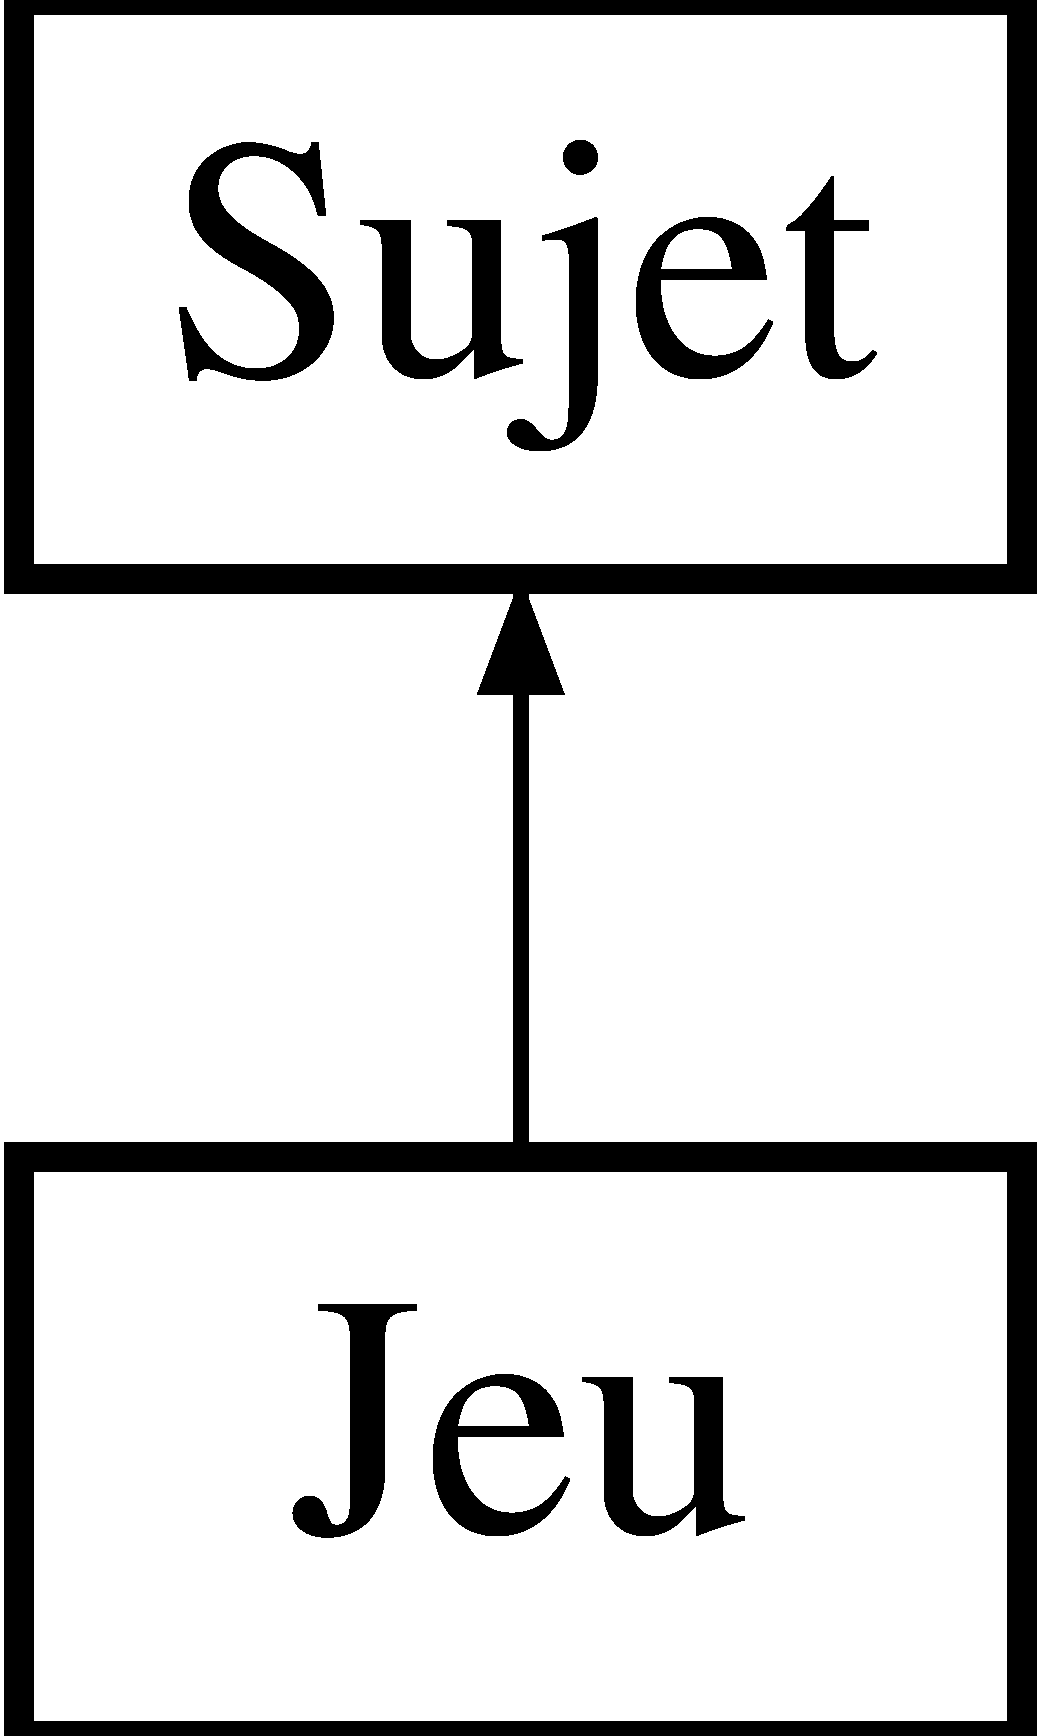
\includegraphics[height=2.000000cm]{class_jeu}
\end{center}
\end{figure}
\subsection*{Fonctions membres publiques}
\begin{DoxyCompactItemize}
\item 
\hyperlink{class_jeu_a3033d02a2ec0e17b170b0735393d716e}{Jeu} (\hyperlink{class_joueur}{Joueur} $\ast$j1, \hyperlink{class_joueur}{Joueur} $\ast$j2)
\item 
\hyperlink{class_jeu_a9cd19e73df169d7f09397be61ba8548c}{$\sim$\-Jeu} ()
\item 
\hyperlink{class_joueur}{Joueur} $\ast$ \hyperlink{class_jeu_a676f11e6bda0cde27f128e90cbaae765}{get\-Joueur\-Courant} ()
\item 
\hyperlink{class_joueur}{Joueur} $\ast$ \hyperlink{class_jeu_aeaa0f199d6a1c9271a49b226159dd1ca}{get\-Joueur\-Autre} ()
\item 
\hyperlink{class_etat}{Etat} $\ast$ \hyperlink{class_jeu_a6a84bec16f8075c1c9b867096dfc2b06}{get\-Etat\-Courant} ()
\item 
\hyperlink{class_etat}{Etat} $\ast$ \hyperlink{class_jeu_a6af6b2d0bd215cde1d63dbe3e799b291}{get\-Etat\-No\-Mana} ()
\item 
\hyperlink{class_etat}{Etat} $\ast$ \hyperlink{class_jeu_a4935a721a0e230cebae3905c78f3721f}{get\-Etat\-No\-Attaque} ()
\item 
\hyperlink{class_etat}{Etat} $\ast$ \hyperlink{class_jeu_a94fc4b05a1d532795b4c8a5d0fec4003}{get\-Etat\-Double\-No} ()
\item 
\hyperlink{class_etat}{Etat} $\ast$ \hyperlink{class_jeu_a8ae205a6a9d95ec5bed20e2fdf5c74a7}{get\-Etat\-Debut\-Tour} ()
\item 
void \hyperlink{class_jeu_a0e5e13b72cd123ac0afef1fa001c9d5f}{set\-Etat} (\hyperlink{class_etat}{Etat} $\ast$e)
\item 
\hyperlink{class_vue_console}{Vue\-Console} $\ast$ \hyperlink{class_jeu_a2f39c9ab947721e35f78a0e187722ce6}{get\-Vue} ()
\item 
void \hyperlink{class_jeu_a86087ecade936bff6bad82eb024ba6bf}{attaque\-Cv\-C} (int index1, int index2)
\item 
void \hyperlink{class_jeu_a81b8b7bc79f9df1b1f3c557e04e8c634}{attaque\-Cv\-J} (int index)
\item 
void \hyperlink{class_jeu_a43c11cf6d659b78dd957cfa65d6d5547}{enlever\-Malinvoc} ()
\item 
bool \hyperlink{class_jeu_abbbc59a98fe8296456ddc112faa2b66b}{test\-No\-Mana} ()
\item 
bool \hyperlink{class_jeu_a391aae052833ebc367a660f4d3a7df29}{test\-Provoc} ()
\item 
bool \hyperlink{class_jeu_a2613ca19004343323262ca2b0d55ca33}{test\-No\-Attaque} ()
\item 
void \hyperlink{class_jeu_a2952107f355b2d0c53bfc2a048c17705}{echange\-Joueur} ()
\item 
void \hyperlink{class_jeu_a042628965e72acf7d4d498aa88f32f1f}{fin\-Tour} ()
\item 
void \hyperlink{class_jeu_a23aa7effc82b36e177013394ee74421e}{jouer} ()
\item 
void \hyperlink{class_jeu_a88bf8ed9150f780b02e70decc60a3f02}{enregistrer\-Obs} (\hyperlink{class_observer}{Observer} $\ast$O)
\item 
void \hyperlink{class_jeu_a8a051ac409a0e53397df3d4578a1e571}{supprimer\-Obs} (\hyperlink{class_observer}{Observer} $\ast$O)
\item 
bool \hyperlink{class_jeu_acd9b7a2de81b5ca7d2a5c3b7e5e177e2}{notifier\-Obs} ()
\item 
void \hyperlink{class_jeu_a97de7b353912bf1754c33c41ea753790}{fonctions\-Carte} (int f)
\end{DoxyCompactItemize}


\subsection{Documentation des constructeurs et destructeur}
\hypertarget{class_jeu_a3033d02a2ec0e17b170b0735393d716e}{\index{Jeu@{Jeu}!Jeu@{Jeu}}
\index{Jeu@{Jeu}!Jeu@{Jeu}}
\subsubsection[{Jeu}]{\setlength{\rightskip}{0pt plus 5cm}Jeu\-::\-Jeu (
\begin{DoxyParamCaption}
\item[{{\bf Joueur} $\ast$}]{j1, }
\item[{{\bf Joueur} $\ast$}]{j2}
\end{DoxyParamCaption}
)}}\label{class_jeu_a3033d02a2ec0e17b170b0735393d716e}
Constructeur 
\begin{DoxyParams}{Paramètres}
{\em j1} & \hyperlink{class_joueur}{Joueur} 1 \\
\hline
{\em j2} & Joueur2 \\
\hline
\end{DoxyParams}
\hypertarget{class_jeu_a9cd19e73df169d7f09397be61ba8548c}{\index{Jeu@{Jeu}!$\sim$\-Jeu@{$\sim$\-Jeu}}
\index{$\sim$\-Jeu@{$\sim$\-Jeu}!Jeu@{Jeu}}
\subsubsection[{$\sim$\-Jeu}]{\setlength{\rightskip}{0pt plus 5cm}Jeu\-::$\sim$\-Jeu (
\begin{DoxyParamCaption}
{}
\end{DoxyParamCaption}
)}}\label{class_jeu_a9cd19e73df169d7f09397be61ba8548c}
Destructeur 

\subsection{Documentation des fonctions membres}
\hypertarget{class_jeu_a86087ecade936bff6bad82eb024ba6bf}{\index{Jeu@{Jeu}!attaque\-Cv\-C@{attaque\-Cv\-C}}
\index{attaque\-Cv\-C@{attaque\-Cv\-C}!Jeu@{Jeu}}
\subsubsection[{attaque\-Cv\-C}]{\setlength{\rightskip}{0pt plus 5cm}void Jeu\-::attaque\-Cv\-C (
\begin{DoxyParamCaption}
\item[{int}]{index1, }
\item[{int}]{index2}
\end{DoxyParamCaption}
)}}\label{class_jeu_a86087ecade936bff6bad82eb024ba6bf}
Méthode qui gère l'attaque d'une \hyperlink{class_carte}{Carte} contre une autre \hyperlink{class_carte}{Carte} 
\begin{DoxyParams}{Paramètres}
{\em index1} & l'index de la carte du joueur courant \\
\hline
{\em index2} & l'index de la carte du joueur adverse \\
\hline
\end{DoxyParams}
\hypertarget{class_jeu_a81b8b7bc79f9df1b1f3c557e04e8c634}{\index{Jeu@{Jeu}!attaque\-Cv\-J@{attaque\-Cv\-J}}
\index{attaque\-Cv\-J@{attaque\-Cv\-J}!Jeu@{Jeu}}
\subsubsection[{attaque\-Cv\-J}]{\setlength{\rightskip}{0pt plus 5cm}void Jeu\-::attaque\-Cv\-J (
\begin{DoxyParamCaption}
\item[{int}]{index1}
\end{DoxyParamCaption}
)}}\label{class_jeu_a81b8b7bc79f9df1b1f3c557e04e8c634}
Méthode qui gère l'attaque d'une \hyperlink{class_carte}{Carte} contre le joueur ennemi. 
\begin{DoxyParams}{Paramètres}
{\em index1} & l'index de la carte du joueur courant. \\
\hline
\end{DoxyParams}
\hypertarget{class_jeu_a2952107f355b2d0c53bfc2a048c17705}{\index{Jeu@{Jeu}!echange\-Joueur@{echange\-Joueur}}
\index{echange\-Joueur@{echange\-Joueur}!Jeu@{Jeu}}
\subsubsection[{echange\-Joueur}]{\setlength{\rightskip}{0pt plus 5cm}void Jeu\-::echange\-Joueur (
\begin{DoxyParamCaption}
{}
\end{DoxyParamCaption}
)}}\label{class_jeu_a2952107f355b2d0c53bfc2a048c17705}
Methode qui echange le joueur\-Courant avec le joueur autre \hypertarget{class_jeu_a43c11cf6d659b78dd957cfa65d6d5547}{\index{Jeu@{Jeu}!enlever\-Malinvoc@{enlever\-Malinvoc}}
\index{enlever\-Malinvoc@{enlever\-Malinvoc}!Jeu@{Jeu}}
\subsubsection[{enlever\-Malinvoc}]{\setlength{\rightskip}{0pt plus 5cm}void Jeu\-::enlever\-Malinvoc (
\begin{DoxyParamCaption}
{}
\end{DoxyParamCaption}
)}}\label{class_jeu_a43c11cf6d659b78dd957cfa65d6d5547}
Méthode utilisée au début du tout d'un jour pour enlever le Mal d'invocation de tout ses serviteurs. \hypertarget{class_jeu_a88bf8ed9150f780b02e70decc60a3f02}{\index{Jeu@{Jeu}!enregistrer\-Obs@{enregistrer\-Obs}}
\index{enregistrer\-Obs@{enregistrer\-Obs}!Jeu@{Jeu}}
\subsubsection[{enregistrer\-Obs}]{\setlength{\rightskip}{0pt plus 5cm}void Jeu\-::enregistrer\-Obs (
\begin{DoxyParamCaption}
\item[{{\bf Observer} $\ast$}]{O}
\end{DoxyParamCaption}
)\hspace{0.3cm}{\ttfamily [virtual]}}}\label{class_jeu_a88bf8ed9150f780b02e70decc60a3f02}
Méthode qui enregistre un \hyperlink{class_observer}{Observer} dans la liste d'Observers. 
\begin{DoxyParams}{Paramètres}
{\em o} & l'\hyperlink{class_observer}{Observer} à ajouter dans la liste. \\
\hline
\end{DoxyParams}


Implémente \hyperlink{class_sujet_aacd8c7455737c41df8fc5ebbea865745}{Sujet}.

\hypertarget{class_jeu_a042628965e72acf7d4d498aa88f32f1f}{\index{Jeu@{Jeu}!fin\-Tour@{fin\-Tour}}
\index{fin\-Tour@{fin\-Tour}!Jeu@{Jeu}}
\subsubsection[{fin\-Tour}]{\setlength{\rightskip}{0pt plus 5cm}void Jeu\-::fin\-Tour (
\begin{DoxyParamCaption}
{}
\end{DoxyParamCaption}
)}}\label{class_jeu_a042628965e72acf7d4d498aa88f32f1f}
Methode qui appelle la méthode \hyperlink{class_jeu_a042628965e72acf7d4d498aa88f32f1f}{fin\-Tour()} sur le tour courant \hypertarget{class_jeu_a97de7b353912bf1754c33c41ea753790}{\index{Jeu@{Jeu}!fonctions\-Carte@{fonctions\-Carte}}
\index{fonctions\-Carte@{fonctions\-Carte}!Jeu@{Jeu}}
\subsubsection[{fonctions\-Carte}]{\setlength{\rightskip}{0pt plus 5cm}void Jeu\-::fonctions\-Carte (
\begin{DoxyParamCaption}
\item[{int}]{f}
\end{DoxyParamCaption}
)}}\label{class_jeu_a97de7b353912bf1754c33c41ea753790}
Méthode qui gère les actions de toutes les cartes sortilège. 
\begin{DoxyParams}{Paramètres}
{\em f} & entier correspondant à un sortilège précis. (attribut de \hyperlink{class_carte}{Carte}) \\
\hline
\end{DoxyParams}
\hypertarget{class_jeu_a6a84bec16f8075c1c9b867096dfc2b06}{\index{Jeu@{Jeu}!get\-Etat\-Courant@{get\-Etat\-Courant}}
\index{get\-Etat\-Courant@{get\-Etat\-Courant}!Jeu@{Jeu}}
\subsubsection[{get\-Etat\-Courant}]{\setlength{\rightskip}{0pt plus 5cm}{\bf Etat} $\ast$ Jeu\-::get\-Etat\-Courant (
\begin{DoxyParamCaption}
{}
\end{DoxyParamCaption}
)}}\label{class_jeu_a6a84bec16f8075c1c9b867096dfc2b06}
Methode qui renvoie l'etat courant \begin{DoxyReturn}{Renvoie}
tour\-Courant l'etat courant 
\end{DoxyReturn}
\hypertarget{class_jeu_a8ae205a6a9d95ec5bed20e2fdf5c74a7}{\index{Jeu@{Jeu}!get\-Etat\-Debut\-Tour@{get\-Etat\-Debut\-Tour}}
\index{get\-Etat\-Debut\-Tour@{get\-Etat\-Debut\-Tour}!Jeu@{Jeu}}
\subsubsection[{get\-Etat\-Debut\-Tour}]{\setlength{\rightskip}{0pt plus 5cm}{\bf Etat} $\ast$ Jeu\-::get\-Etat\-Debut\-Tour (
\begin{DoxyParamCaption}
{}
\end{DoxyParamCaption}
)}}\label{class_jeu_a8ae205a6a9d95ec5bed20e2fdf5c74a7}
Methode qui renvoie l'etat Debut\-Tour \begin{DoxyReturn}{Renvoie}
etat\-Debut\-Tour l'etat Debut\-Tour 
\end{DoxyReturn}
\hypertarget{class_jeu_a94fc4b05a1d532795b4c8a5d0fec4003}{\index{Jeu@{Jeu}!get\-Etat\-Double\-No@{get\-Etat\-Double\-No}}
\index{get\-Etat\-Double\-No@{get\-Etat\-Double\-No}!Jeu@{Jeu}}
\subsubsection[{get\-Etat\-Double\-No}]{\setlength{\rightskip}{0pt plus 5cm}{\bf Etat} $\ast$ Jeu\-::get\-Etat\-Double\-No (
\begin{DoxyParamCaption}
{}
\end{DoxyParamCaption}
)}}\label{class_jeu_a94fc4b05a1d532795b4c8a5d0fec4003}
Methode qui renvoie l'etat Double\-No \begin{DoxyReturn}{Renvoie}
etat\-Double\-No l'etat Double\-No 
\end{DoxyReturn}
\hypertarget{class_jeu_a4935a721a0e230cebae3905c78f3721f}{\index{Jeu@{Jeu}!get\-Etat\-No\-Attaque@{get\-Etat\-No\-Attaque}}
\index{get\-Etat\-No\-Attaque@{get\-Etat\-No\-Attaque}!Jeu@{Jeu}}
\subsubsection[{get\-Etat\-No\-Attaque}]{\setlength{\rightskip}{0pt plus 5cm}{\bf Etat} $\ast$ Jeu\-::get\-Etat\-No\-Attaque (
\begin{DoxyParamCaption}
{}
\end{DoxyParamCaption}
)}}\label{class_jeu_a4935a721a0e230cebae3905c78f3721f}
Methode qui renvoie l'etat No\-Attaque \begin{DoxyReturn}{Renvoie}
etat\-No\-Attaque l'etat No\-Attaque 
\end{DoxyReturn}
\hypertarget{class_jeu_a6af6b2d0bd215cde1d63dbe3e799b291}{\index{Jeu@{Jeu}!get\-Etat\-No\-Mana@{get\-Etat\-No\-Mana}}
\index{get\-Etat\-No\-Mana@{get\-Etat\-No\-Mana}!Jeu@{Jeu}}
\subsubsection[{get\-Etat\-No\-Mana}]{\setlength{\rightskip}{0pt plus 5cm}{\bf Etat} $\ast$ Jeu\-::get\-Etat\-No\-Mana (
\begin{DoxyParamCaption}
{}
\end{DoxyParamCaption}
)}}\label{class_jeu_a6af6b2d0bd215cde1d63dbe3e799b291}
Methode qui renvoie l'etat No\-Mana \begin{DoxyReturn}{Renvoie}
etat\-No\-Mana l'etat no mana 
\end{DoxyReturn}
\hypertarget{class_jeu_aeaa0f199d6a1c9271a49b226159dd1ca}{\index{Jeu@{Jeu}!get\-Joueur\-Autre@{get\-Joueur\-Autre}}
\index{get\-Joueur\-Autre@{get\-Joueur\-Autre}!Jeu@{Jeu}}
\subsubsection[{get\-Joueur\-Autre}]{\setlength{\rightskip}{0pt plus 5cm}{\bf Joueur} $\ast$ Jeu\-::get\-Joueur\-Autre (
\begin{DoxyParamCaption}
{}
\end{DoxyParamCaption}
)}}\label{class_jeu_aeaa0f199d6a1c9271a49b226159dd1ca}
Methode qui retourne le joueur autre \begin{DoxyReturn}{Renvoie}
joueur\-Autre le joueur autre 
\end{DoxyReturn}
\hypertarget{class_jeu_a676f11e6bda0cde27f128e90cbaae765}{\index{Jeu@{Jeu}!get\-Joueur\-Courant@{get\-Joueur\-Courant}}
\index{get\-Joueur\-Courant@{get\-Joueur\-Courant}!Jeu@{Jeu}}
\subsubsection[{get\-Joueur\-Courant}]{\setlength{\rightskip}{0pt plus 5cm}{\bf Joueur} $\ast$ Jeu\-::get\-Joueur\-Courant (
\begin{DoxyParamCaption}
{}
\end{DoxyParamCaption}
)}}\label{class_jeu_a676f11e6bda0cde27f128e90cbaae765}
Methode qui retourne le joueur courant \begin{DoxyReturn}{Renvoie}
joueur\-Courant le joueur courant 
\end{DoxyReturn}
\hypertarget{class_jeu_a2f39c9ab947721e35f78a0e187722ce6}{\index{Jeu@{Jeu}!get\-Vue@{get\-Vue}}
\index{get\-Vue@{get\-Vue}!Jeu@{Jeu}}
\subsubsection[{get\-Vue}]{\setlength{\rightskip}{0pt plus 5cm}{\bf Vue\-Console} $\ast$ Jeu\-::get\-Vue (
\begin{DoxyParamCaption}
{}
\end{DoxyParamCaption}
)}}\label{class_jeu_a2f39c9ab947721e35f78a0e187722ce6}
Methode qui retourne la vue \begin{DoxyReturn}{Renvoie}
vue la vue 
\end{DoxyReturn}
\hypertarget{class_jeu_a23aa7effc82b36e177013394ee74421e}{\index{Jeu@{Jeu}!jouer@{jouer}}
\index{jouer@{jouer}!Jeu@{Jeu}}
\subsubsection[{jouer}]{\setlength{\rightskip}{0pt plus 5cm}void Jeu\-::jouer (
\begin{DoxyParamCaption}
{}
\end{DoxyParamCaption}
)}}\label{class_jeu_a23aa7effc82b36e177013394ee74421e}
Methode qui lance le jeu \hypertarget{class_jeu_acd9b7a2de81b5ca7d2a5c3b7e5e177e2}{\index{Jeu@{Jeu}!notifier\-Obs@{notifier\-Obs}}
\index{notifier\-Obs@{notifier\-Obs}!Jeu@{Jeu}}
\subsubsection[{notifier\-Obs}]{\setlength{\rightskip}{0pt plus 5cm}bool Jeu\-::notifier\-Obs (
\begin{DoxyParamCaption}
{}
\end{DoxyParamCaption}
)\hspace{0.3cm}{\ttfamily [virtual]}}}\label{class_jeu_acd9b7a2de81b5ca7d2a5c3b7e5e177e2}
Méthode qui actualise tout les Observers de la liste d'Observers. 

Implémente \hyperlink{class_sujet_a210b37440cb4dbb5eff2770a44c14b0d}{Sujet}.

\hypertarget{class_jeu_a0e5e13b72cd123ac0afef1fa001c9d5f}{\index{Jeu@{Jeu}!set\-Etat@{set\-Etat}}
\index{set\-Etat@{set\-Etat}!Jeu@{Jeu}}
\subsubsection[{set\-Etat}]{\setlength{\rightskip}{0pt plus 5cm}void Jeu\-::set\-Etat (
\begin{DoxyParamCaption}
\item[{{\bf Etat} $\ast$}]{e}
\end{DoxyParamCaption}
)}}\label{class_jeu_a0e5e13b72cd123ac0afef1fa001c9d5f}
Methode qui change l'etat courant 
\begin{DoxyParams}{Paramètres}
{\em e} & le nouvel etat \\
\hline
\end{DoxyParams}
\hypertarget{class_jeu_a8a051ac409a0e53397df3d4578a1e571}{\index{Jeu@{Jeu}!supprimer\-Obs@{supprimer\-Obs}}
\index{supprimer\-Obs@{supprimer\-Obs}!Jeu@{Jeu}}
\subsubsection[{supprimer\-Obs}]{\setlength{\rightskip}{0pt plus 5cm}void Jeu\-::supprimer\-Obs (
\begin{DoxyParamCaption}
\item[{{\bf Observer} $\ast$}]{O}
\end{DoxyParamCaption}
)\hspace{0.3cm}{\ttfamily [virtual]}}}\label{class_jeu_a8a051ac409a0e53397df3d4578a1e571}
Méthode qui supprime un \hyperlink{class_observer}{Observer} de la liste d'Observers. 
\begin{DoxyParams}{Paramètres}
{\em o} & l'\hyperlink{class_observer}{Observer} à supprimer dans la liste. \\
\hline
\end{DoxyParams}


Implémente \hyperlink{class_sujet_a6d121bdc49579675064cfd038b751922}{Sujet}.

\hypertarget{class_jeu_a2613ca19004343323262ca2b0d55ca33}{\index{Jeu@{Jeu}!test\-No\-Attaque@{test\-No\-Attaque}}
\index{test\-No\-Attaque@{test\-No\-Attaque}!Jeu@{Jeu}}
\subsubsection[{test\-No\-Attaque}]{\setlength{\rightskip}{0pt plus 5cm}bool Jeu\-::test\-No\-Attaque (
\begin{DoxyParamCaption}
{}
\end{DoxyParamCaption}
)}}\label{class_jeu_a2613ca19004343323262ca2b0d55ca33}
Méthode qui teste si le \hyperlink{class_joueur}{Joueur} possède des Serviteurs qui peuvent attaquer. \begin{DoxyReturn}{Renvoie}
noatt , true si tout les serviteurs ne peuvent plus attaquer, false si au moins un serviteur peut attaquer. 
\end{DoxyReturn}
\hypertarget{class_jeu_abbbc59a98fe8296456ddc112faa2b66b}{\index{Jeu@{Jeu}!test\-No\-Mana@{test\-No\-Mana}}
\index{test\-No\-Mana@{test\-No\-Mana}!Jeu@{Jeu}}
\subsubsection[{test\-No\-Mana}]{\setlength{\rightskip}{0pt plus 5cm}bool Jeu\-::test\-No\-Mana (
\begin{DoxyParamCaption}
{}
\end{DoxyParamCaption}
)}}\label{class_jeu_abbbc59a98fe8296456ddc112faa2b66b}
Méthode qui teste si le \hyperlink{class_joueur}{Joueur} a assez de mana pour continuer de faire des actions. \begin{DoxyReturn}{Renvoie}
nomana , true si le \hyperlink{class_joueur}{Joueur} na plus assez de Mana, false si le \hyperlink{class_joueur}{Joueur} a suffisamment de Mana. 
\end{DoxyReturn}
\hypertarget{class_jeu_a391aae052833ebc367a660f4d3a7df29}{\index{Jeu@{Jeu}!test\-Provoc@{test\-Provoc}}
\index{test\-Provoc@{test\-Provoc}!Jeu@{Jeu}}
\subsubsection[{test\-Provoc}]{\setlength{\rightskip}{0pt plus 5cm}bool Jeu\-::test\-Provoc (
\begin{DoxyParamCaption}
{}
\end{DoxyParamCaption}
)}}\label{class_jeu_a391aae052833ebc367a660f4d3a7df29}
Méthode qui teste si le \hyperlink{class_joueur}{Joueur} adverse possède des serviteurs avec Provocation. \begin{DoxyReturn}{Renvoie}
provoc , true si le \hyperlink{class_joueur}{Joueur} adverse a au moins un serviteur avec Provocation, false si le \hyperlink{class_joueur}{Joueur} adverse n'a pas de serviteurs avec Provocation. 
\end{DoxyReturn}


La documentation de cette classe a été générée à partir des fichiers suivants \-:\begin{DoxyCompactItemize}
\item 
include/\-Controleur/\hyperlink{_jeu_8hpp}{Jeu.\-hpp}\item 
src/\-Controleur/\hyperlink{_jeu_8cpp}{Jeu.\-cpp}\end{DoxyCompactItemize}

\hypertarget{class_joueur}{\section{Référence de la classe Joueur}
\label{class_joueur}\index{Joueur@{Joueur}}
}


{\ttfamily \#include $<$Joueur.\-hpp$>$}

Graphe d'héritage de Joueur\-:\begin{figure}[H]
\begin{center}
\leavevmode
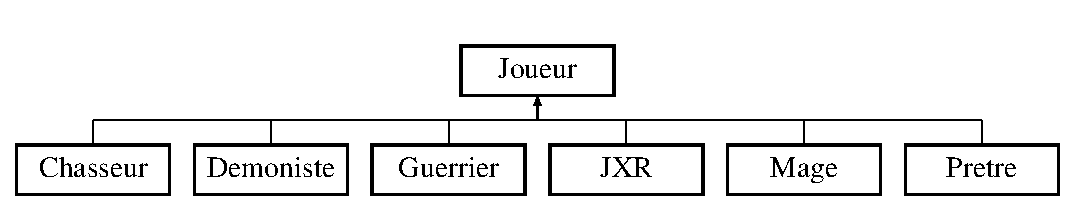
\includegraphics[height=2.000000cm]{class_joueur}
\end{center}
\end{figure}
\subsection*{Fonctions membres publiques}
\begin{DoxyCompactItemize}
\item 
\hyperlink{class_joueur_a055a0bc38f47a424243d44e7078af129}{Joueur} (std\-::string nom, std\-::string fichier)
\item 
\hyperlink{class_joueur_a9fb594f755601ee77ce5884c4c0861f3}{$\sim$\-Joueur} ()
\item 
int \hyperlink{class_joueur_a3deefa81ebbb921d6cef52322777dee7}{get\-Pdv} ()
\item 
int \hyperlink{class_joueur_adab9394b18e1e65a77aa8dad7b51ec28}{get\-Armure} ()
\item 
void \hyperlink{class_joueur_a2ff017f6e65cad383d00d153ece08045}{set\-A\-R\-M\-U\-R\-E} (int arm)
\item 
int \hyperlink{class_joueur_ac950c36b21e1dfc7038d9bb4e1f53361}{get\-Pdm} ()
\item 
void \hyperlink{class_joueur_a199d04e5240f4078ba2f3da2431f0bb2}{set\-P\-D\-M} (int npdm)
\item 
int \hyperlink{class_joueur_ab9297495de7521ac2198c7ce8d38191c}{get\-Pdm\-Tour} ()
\item 
void \hyperlink{class_joueur_a3984848768db7e175aeeb51ca89e4eb3}{set\-P\-D\-M\-Tour} (int npdmt)
\item 
void \hyperlink{class_joueur_ac4b9408bed0a64ac63188f7f8e1a73d9}{set\-P\-D\-V} (int npdv)
\item 
std\-::string \hyperlink{class_joueur_a5ba8036208a35efd6bf37a86b36063b0}{get\-Nom} ()
\item 
void \hyperlink{class_joueur_afa24ba80453522ff059e7e6f46653749}{set\-Nom} (std\-::string n)
\item 
\hyperlink{class_joueur}{Joueur} $\ast$ \hyperlink{class_joueur_a0a2f88581ef12441b03a1cc4ed721b40}{get\-Joueur\-Autre} ()
\item 
void \hyperlink{class_joueur_a81aa9fca9a001be893bfaa607681b086}{set\-Joueur\-Autre} (\hyperlink{class_joueur}{Joueur} $\ast$j)
\item 
\hyperlink{class_comportement_pouvoir}{Comportement\-Pouvoir} $\ast$ \hyperlink{class_joueur_a85df9863c4257fe7405a6b1fe7c1e1ef}{get\-C\-P} ()
\item 
void \hyperlink{class_joueur_a7b408ea957e1b125a509ec8e88b2c148}{set\-C\-P} (\hyperlink{class_comportement_pouvoir}{Comportement\-Pouvoir} $\ast$C\-P)
\item 
std\-::string \hyperlink{class_joueur_a99e2e0934bb9307f577d9fa3f219a7b6}{to\-String} ()
\item 
void \hyperlink{class_joueur_a91239ad650edadbee5b1b51d19242d28}{utiliser\-Pouvoir} ()
\item 
bool \hyperlink{class_joueur_a0344bd2b30346f73e23239b62647e26d}{get\-Pouvoir\-Utilise} ()
\item 
void \hyperlink{class_joueur_a57f6f8d3ff6ba9b5026a51b23e03cd0a}{set\-Pouvoir\-Utilise} (bool p)
\item 
\hyperlink{class_deck}{Deck} $\ast$ \hyperlink{class_joueur_a5f7a140f00766144edf7d6a5b0f236b7}{get\-Deck} ()
\item 
std\-::vector$<$ \hyperlink{class_carte}{Carte} $>$ $\ast$ \hyperlink{class_joueur_a569fa77a585a0e82981bfa6bda149a4f}{get\-Main} ()
\item 
std\-::vector$<$ \hyperlink{class_carte}{Carte} $>$ $\ast$ \hyperlink{class_joueur_abe6504e86cf56787e5569c296e3bfde7}{get\-Board} ()
\item 
bool \hyperlink{class_joueur_a0b94001f3dd61af944bd7128d143ac11}{ajouter\-Main} (\hyperlink{class_carte}{Carte} c)
\item 
bool \hyperlink{class_joueur_a5046cd3251b93c58558ca273db1aa23b}{ajouter\-Board} (\hyperlink{class_carte}{Carte} c)
\item 
bool \hyperlink{class_joueur_ae1c641d98c6e9fda547c3b7e923f085e}{supprimer\-Main} (int index)
\item 
bool \hyperlink{class_joueur_af086855b254a628bc9c07047142fb33c}{supprimer\-Board} (int index)
\item 
std\-::string \hyperlink{class_joueur_a4a41ec6aaa2e7b4a55807b86cc286876}{afficher\-Main} ()
\item 
std\-::string \hyperlink{class_joueur_aae890e668b097dddee94a61404553c8f}{afficher\-Board} ()
\end{DoxyCompactItemize}


\subsection{Documentation des constructeurs et destructeur}
\hypertarget{class_joueur_a055a0bc38f47a424243d44e7078af129}{\index{Joueur@{Joueur}!Joueur@{Joueur}}
\index{Joueur@{Joueur}!Joueur@{Joueur}}
\subsubsection[{Joueur}]{\setlength{\rightskip}{0pt plus 5cm}Joueur\-::\-Joueur (
\begin{DoxyParamCaption}
\item[{std\-::string}]{nom, }
\item[{std\-::string}]{fichier}
\end{DoxyParamCaption}
)}}\label{class_joueur_a055a0bc38f47a424243d44e7078af129}
Constructeur. 
\begin{DoxyParams}{Paramètres}
{\em nom} & string le nom du joueur \\
\hline
{\em fichier} & string le fichier utilisé pour creer le deck \\
\hline
\end{DoxyParams}
\hypertarget{class_joueur_a9fb594f755601ee77ce5884c4c0861f3}{\index{Joueur@{Joueur}!$\sim$\-Joueur@{$\sim$\-Joueur}}
\index{$\sim$\-Joueur@{$\sim$\-Joueur}!Joueur@{Joueur}}
\subsubsection[{$\sim$\-Joueur}]{\setlength{\rightskip}{0pt plus 5cm}Joueur\-::$\sim$\-Joueur (
\begin{DoxyParamCaption}
{}
\end{DoxyParamCaption}
)}}\label{class_joueur_a9fb594f755601ee77ce5884c4c0861f3}
Destructeur. 

\subsection{Documentation des fonctions membres}
\hypertarget{class_joueur_aae890e668b097dddee94a61404553c8f}{\index{Joueur@{Joueur}!afficher\-Board@{afficher\-Board}}
\index{afficher\-Board@{afficher\-Board}!Joueur@{Joueur}}
\subsubsection[{afficher\-Board}]{\setlength{\rightskip}{0pt plus 5cm}string Joueur\-::afficher\-Board (
\begin{DoxyParamCaption}
{}
\end{DoxyParamCaption}
)}}\label{class_joueur_aae890e668b097dddee94a61404553c8f}
\hypertarget{class_joueur_a4a41ec6aaa2e7b4a55807b86cc286876}{\index{Joueur@{Joueur}!afficher\-Main@{afficher\-Main}}
\index{afficher\-Main@{afficher\-Main}!Joueur@{Joueur}}
\subsubsection[{afficher\-Main}]{\setlength{\rightskip}{0pt plus 5cm}string Joueur\-::afficher\-Main (
\begin{DoxyParamCaption}
{}
\end{DoxyParamCaption}
)}}\label{class_joueur_a4a41ec6aaa2e7b4a55807b86cc286876}
\hypertarget{class_joueur_a5046cd3251b93c58558ca273db1aa23b}{\index{Joueur@{Joueur}!ajouter\-Board@{ajouter\-Board}}
\index{ajouter\-Board@{ajouter\-Board}!Joueur@{Joueur}}
\subsubsection[{ajouter\-Board}]{\setlength{\rightskip}{0pt plus 5cm}bool Joueur\-::ajouter\-Board (
\begin{DoxyParamCaption}
\item[{{\bf Carte}}]{c}
\end{DoxyParamCaption}
)}}\label{class_joueur_a5046cd3251b93c58558ca273db1aa23b}
\hypertarget{class_joueur_a0b94001f3dd61af944bd7128d143ac11}{\index{Joueur@{Joueur}!ajouter\-Main@{ajouter\-Main}}
\index{ajouter\-Main@{ajouter\-Main}!Joueur@{Joueur}}
\subsubsection[{ajouter\-Main}]{\setlength{\rightskip}{0pt plus 5cm}bool Joueur\-::ajouter\-Main (
\begin{DoxyParamCaption}
\item[{{\bf Carte}}]{c}
\end{DoxyParamCaption}
)}}\label{class_joueur_a0b94001f3dd61af944bd7128d143ac11}
\hypertarget{class_joueur_adab9394b18e1e65a77aa8dad7b51ec28}{\index{Joueur@{Joueur}!get\-Armure@{get\-Armure}}
\index{get\-Armure@{get\-Armure}!Joueur@{Joueur}}
\subsubsection[{get\-Armure}]{\setlength{\rightskip}{0pt plus 5cm}int Joueur\-::get\-Armure (
\begin{DoxyParamCaption}
{}
\end{DoxyParamCaption}
)}}\label{class_joueur_adab9394b18e1e65a77aa8dad7b51ec28}
Methode qui renvoie le nombre de points d''armure du personnage \begin{DoxyReturn}{Renvoie}
armure les points d'armure du personnage 
\end{DoxyReturn}
\hypertarget{class_joueur_abe6504e86cf56787e5569c296e3bfde7}{\index{Joueur@{Joueur}!get\-Board@{get\-Board}}
\index{get\-Board@{get\-Board}!Joueur@{Joueur}}
\subsubsection[{get\-Board}]{\setlength{\rightskip}{0pt plus 5cm}vector$<$ {\bf Carte} $>$ $\ast$ Joueur\-::get\-Board (
\begin{DoxyParamCaption}
{}
\end{DoxyParamCaption}
)}}\label{class_joueur_abe6504e86cf56787e5569c296e3bfde7}
Methode qui renvoie les pv de la carte \begin{DoxyReturn}{Renvoie}
pdv int les points de vie de la carte 
\end{DoxyReturn}
\hypertarget{class_joueur_a85df9863c4257fe7405a6b1fe7c1e1ef}{\index{Joueur@{Joueur}!get\-C\-P@{get\-C\-P}}
\index{get\-C\-P@{get\-C\-P}!Joueur@{Joueur}}
\subsubsection[{get\-C\-P}]{\setlength{\rightskip}{0pt plus 5cm}{\bf Comportement\-Pouvoir} $\ast$ Joueur\-::get\-C\-P (
\begin{DoxyParamCaption}
{}
\end{DoxyParamCaption}
)}}\label{class_joueur_a85df9863c4257fe7405a6b1fe7c1e1ef}
Methode qui renvoie le comportement du pouvoir du personnage \begin{DoxyReturn}{Renvoie}
C\-P le comportement du pouvoir du personnage 
\end{DoxyReturn}
\hypertarget{class_joueur_a5f7a140f00766144edf7d6a5b0f236b7}{\index{Joueur@{Joueur}!get\-Deck@{get\-Deck}}
\index{get\-Deck@{get\-Deck}!Joueur@{Joueur}}
\subsubsection[{get\-Deck}]{\setlength{\rightskip}{0pt plus 5cm}{\bf Deck} $\ast$ Joueur\-::get\-Deck (
\begin{DoxyParamCaption}
{}
\end{DoxyParamCaption}
)}}\label{class_joueur_a5f7a140f00766144edf7d6a5b0f236b7}
Methode qui renvoie le deck du joueur \begin{DoxyReturn}{Renvoie}
d \hyperlink{class_deck}{Deck} le deck du \hyperlink{class_joueur}{Joueur} 
\end{DoxyReturn}
\hypertarget{class_joueur_a0a2f88581ef12441b03a1cc4ed721b40}{\index{Joueur@{Joueur}!get\-Joueur\-Autre@{get\-Joueur\-Autre}}
\index{get\-Joueur\-Autre@{get\-Joueur\-Autre}!Joueur@{Joueur}}
\subsubsection[{get\-Joueur\-Autre}]{\setlength{\rightskip}{0pt plus 5cm}{\bf Joueur} $\ast$ Joueur\-::get\-Joueur\-Autre (
\begin{DoxyParamCaption}
{}
\end{DoxyParamCaption}
)}}\label{class_joueur_a0a2f88581ef12441b03a1cc4ed721b40}
Methode qui renvoie le comportement du pouvoir du personnage \begin{DoxyReturn}{Renvoie}
C\-P le comportement du pouvoir du personnage 
\end{DoxyReturn}
\hypertarget{class_joueur_a569fa77a585a0e82981bfa6bda149a4f}{\index{Joueur@{Joueur}!get\-Main@{get\-Main}}
\index{get\-Main@{get\-Main}!Joueur@{Joueur}}
\subsubsection[{get\-Main}]{\setlength{\rightskip}{0pt plus 5cm}vector$<$ {\bf Carte} $>$ $\ast$ Joueur\-::get\-Main (
\begin{DoxyParamCaption}
{}
\end{DoxyParamCaption}
)}}\label{class_joueur_a569fa77a585a0e82981bfa6bda149a4f}
Methode qui renvoie la main du joueur \begin{DoxyReturn}{Renvoie}
main Vector$<$\-Carte$>$ la main du joueur 
\end{DoxyReturn}
\hypertarget{class_joueur_a5ba8036208a35efd6bf37a86b36063b0}{\index{Joueur@{Joueur}!get\-Nom@{get\-Nom}}
\index{get\-Nom@{get\-Nom}!Joueur@{Joueur}}
\subsubsection[{get\-Nom}]{\setlength{\rightskip}{0pt plus 5cm}std\-::string Joueur\-::get\-Nom (
\begin{DoxyParamCaption}
{}
\end{DoxyParamCaption}
)}}\label{class_joueur_a5ba8036208a35efd6bf37a86b36063b0}
Methode qui renvoie les pv de la carte \begin{DoxyReturn}{Renvoie}
pdv int les points de vie de la carte 
\end{DoxyReturn}
\hypertarget{class_joueur_ac950c36b21e1dfc7038d9bb4e1f53361}{\index{Joueur@{Joueur}!get\-Pdm@{get\-Pdm}}
\index{get\-Pdm@{get\-Pdm}!Joueur@{Joueur}}
\subsubsection[{get\-Pdm}]{\setlength{\rightskip}{0pt plus 5cm}int Joueur\-::get\-Pdm (
\begin{DoxyParamCaption}
{}
\end{DoxyParamCaption}
)}}\label{class_joueur_ac950c36b21e1dfc7038d9bb4e1f53361}
Methode qui renvoie le nombre de points de mana du personnage \begin{DoxyReturn}{Renvoie}
mana les points de mana du personnage 
\end{DoxyReturn}
\hypertarget{class_joueur_ab9297495de7521ac2198c7ce8d38191c}{\index{Joueur@{Joueur}!get\-Pdm\-Tour@{get\-Pdm\-Tour}}
\index{get\-Pdm\-Tour@{get\-Pdm\-Tour}!Joueur@{Joueur}}
\subsubsection[{get\-Pdm\-Tour}]{\setlength{\rightskip}{0pt plus 5cm}int Joueur\-::get\-Pdm\-Tour (
\begin{DoxyParamCaption}
{}
\end{DoxyParamCaption}
)}}\label{class_joueur_ab9297495de7521ac2198c7ce8d38191c}
Methode qui renvoie le nombre de points de mana du personnage au Tour courant \begin{DoxyReturn}{Renvoie}
mana les points de mana du personnage 
\end{DoxyReturn}
\hypertarget{class_joueur_a3deefa81ebbb921d6cef52322777dee7}{\index{Joueur@{Joueur}!get\-Pdv@{get\-Pdv}}
\index{get\-Pdv@{get\-Pdv}!Joueur@{Joueur}}
\subsubsection[{get\-Pdv}]{\setlength{\rightskip}{0pt plus 5cm}int Joueur\-::get\-Pdv (
\begin{DoxyParamCaption}
{}
\end{DoxyParamCaption}
)}}\label{class_joueur_a3deefa81ebbb921d6cef52322777dee7}
Methode qui renvoie le nombre de points de vie du personnage \begin{DoxyReturn}{Renvoie}
pdv les points de vie du personnage 
\end{DoxyReturn}
\hypertarget{class_joueur_a0344bd2b30346f73e23239b62647e26d}{\index{Joueur@{Joueur}!get\-Pouvoir\-Utilise@{get\-Pouvoir\-Utilise}}
\index{get\-Pouvoir\-Utilise@{get\-Pouvoir\-Utilise}!Joueur@{Joueur}}
\subsubsection[{get\-Pouvoir\-Utilise}]{\setlength{\rightskip}{0pt plus 5cm}bool Joueur\-::get\-Pouvoir\-Utilise (
\begin{DoxyParamCaption}
{}
\end{DoxyParamCaption}
)}}\label{class_joueur_a0344bd2b30346f73e23239b62647e26d}
Methode qui renvoie un booléen qui indique si le pouvoir a été utilisé \begin{DoxyReturn}{Renvoie}
pouvoir\-Utilise Booléen etat de l'utilisation du pouvoir 
\end{DoxyReturn}
\hypertarget{class_joueur_a2ff017f6e65cad383d00d153ece08045}{\index{Joueur@{Joueur}!set\-A\-R\-M\-U\-R\-E@{set\-A\-R\-M\-U\-R\-E}}
\index{set\-A\-R\-M\-U\-R\-E@{set\-A\-R\-M\-U\-R\-E}!Joueur@{Joueur}}
\subsubsection[{set\-A\-R\-M\-U\-R\-E}]{\setlength{\rightskip}{0pt plus 5cm}void Joueur\-::set\-A\-R\-M\-U\-R\-E (
\begin{DoxyParamCaption}
\item[{int}]{narmure}
\end{DoxyParamCaption}
)}}\label{class_joueur_a2ff017f6e65cad383d00d153ece08045}
Methode qui remplace les points d'armure du personnage par narmure 
\begin{DoxyParams}{Paramètres}
{\em narmure} & les nouveaux points d'armure \\
\hline
\end{DoxyParams}
\hypertarget{class_joueur_a7b408ea957e1b125a509ec8e88b2c148}{\index{Joueur@{Joueur}!set\-C\-P@{set\-C\-P}}
\index{set\-C\-P@{set\-C\-P}!Joueur@{Joueur}}
\subsubsection[{set\-C\-P}]{\setlength{\rightskip}{0pt plus 5cm}void Joueur\-::set\-C\-P (
\begin{DoxyParamCaption}
\item[{{\bf Comportement\-Pouvoir} $\ast$}]{C\-P}
\end{DoxyParamCaption}
)}}\label{class_joueur_a7b408ea957e1b125a509ec8e88b2c148}
\hypertarget{class_joueur_a81aa9fca9a001be893bfaa607681b086}{\index{Joueur@{Joueur}!set\-Joueur\-Autre@{set\-Joueur\-Autre}}
\index{set\-Joueur\-Autre@{set\-Joueur\-Autre}!Joueur@{Joueur}}
\subsubsection[{set\-Joueur\-Autre}]{\setlength{\rightskip}{0pt plus 5cm}void Joueur\-::set\-Joueur\-Autre (
\begin{DoxyParamCaption}
\item[{{\bf Joueur} $\ast$}]{j}
\end{DoxyParamCaption}
)}}\label{class_joueur_a81aa9fca9a001be893bfaa607681b086}
\hypertarget{class_joueur_afa24ba80453522ff059e7e6f46653749}{\index{Joueur@{Joueur}!set\-Nom@{set\-Nom}}
\index{set\-Nom@{set\-Nom}!Joueur@{Joueur}}
\subsubsection[{set\-Nom}]{\setlength{\rightskip}{0pt plus 5cm}void Joueur\-::set\-Nom (
\begin{DoxyParamCaption}
\item[{std\-::string}]{n}
\end{DoxyParamCaption}
)}}\label{class_joueur_afa24ba80453522ff059e7e6f46653749}
Methode qui modifie le nom du joueur 
\begin{DoxyParams}{Paramètres}
{\em n} & string le nouveau nom du joueur \\
\hline
\end{DoxyParams}
\hypertarget{class_joueur_a199d04e5240f4078ba2f3da2431f0bb2}{\index{Joueur@{Joueur}!set\-P\-D\-M@{set\-P\-D\-M}}
\index{set\-P\-D\-M@{set\-P\-D\-M}!Joueur@{Joueur}}
\subsubsection[{set\-P\-D\-M}]{\setlength{\rightskip}{0pt plus 5cm}void Joueur\-::set\-P\-D\-M (
\begin{DoxyParamCaption}
\item[{int}]{npdm}
\end{DoxyParamCaption}
)}}\label{class_joueur_a199d04e5240f4078ba2f3da2431f0bb2}
Methode qui remplace les points de mana du personnage par npdv 
\begin{DoxyParams}{Paramètres}
{\em npdm} & les nouveaux points de mana \\
\hline
\end{DoxyParams}
\hypertarget{class_joueur_a3984848768db7e175aeeb51ca89e4eb3}{\index{Joueur@{Joueur}!set\-P\-D\-M\-Tour@{set\-P\-D\-M\-Tour}}
\index{set\-P\-D\-M\-Tour@{set\-P\-D\-M\-Tour}!Joueur@{Joueur}}
\subsubsection[{set\-P\-D\-M\-Tour}]{\setlength{\rightskip}{0pt plus 5cm}void Joueur\-::set\-P\-D\-M\-Tour (
\begin{DoxyParamCaption}
\item[{int}]{npdmt}
\end{DoxyParamCaption}
)}}\label{class_joueur_a3984848768db7e175aeeb51ca89e4eb3}
Methode qui remplace les points de mana du personnage par npdv 
\begin{DoxyParams}{Paramètres}
{\em npdm} & les nouveaux points de mana \\
\hline
\end{DoxyParams}
\hypertarget{class_joueur_ac4b9408bed0a64ac63188f7f8e1a73d9}{\index{Joueur@{Joueur}!set\-P\-D\-V@{set\-P\-D\-V}}
\index{set\-P\-D\-V@{set\-P\-D\-V}!Joueur@{Joueur}}
\subsubsection[{set\-P\-D\-V}]{\setlength{\rightskip}{0pt plus 5cm}void Joueur\-::set\-P\-D\-V (
\begin{DoxyParamCaption}
\item[{int}]{npdv}
\end{DoxyParamCaption}
)}}\label{class_joueur_ac4b9408bed0a64ac63188f7f8e1a73d9}
Methode qui remplace les points de vie du personnage par npdv 
\begin{DoxyParams}{Paramètres}
{\em npdv} & les nouveaux points de vie \\
\hline
\end{DoxyParams}
\hypertarget{class_joueur_a57f6f8d3ff6ba9b5026a51b23e03cd0a}{\index{Joueur@{Joueur}!set\-Pouvoir\-Utilise@{set\-Pouvoir\-Utilise}}
\index{set\-Pouvoir\-Utilise@{set\-Pouvoir\-Utilise}!Joueur@{Joueur}}
\subsubsection[{set\-Pouvoir\-Utilise}]{\setlength{\rightskip}{0pt plus 5cm}void Joueur\-::set\-Pouvoir\-Utilise (
\begin{DoxyParamCaption}
\item[{bool}]{p}
\end{DoxyParamCaption}
)}}\label{class_joueur_a57f6f8d3ff6ba9b5026a51b23e03cd0a}
Methode qui modifie le booléen qui indique si le pouvoir a été utilisé 
\begin{DoxyParams}{Paramètres}
{\em p} & Booléen etat de l'utilisation du pouvoir \\
\hline
\end{DoxyParams}
\hypertarget{class_joueur_af086855b254a628bc9c07047142fb33c}{\index{Joueur@{Joueur}!supprimer\-Board@{supprimer\-Board}}
\index{supprimer\-Board@{supprimer\-Board}!Joueur@{Joueur}}
\subsubsection[{supprimer\-Board}]{\setlength{\rightskip}{0pt plus 5cm}bool Joueur\-::supprimer\-Board (
\begin{DoxyParamCaption}
\item[{int}]{index}
\end{DoxyParamCaption}
)}}\label{class_joueur_af086855b254a628bc9c07047142fb33c}
\hypertarget{class_joueur_ae1c641d98c6e9fda547c3b7e923f085e}{\index{Joueur@{Joueur}!supprimer\-Main@{supprimer\-Main}}
\index{supprimer\-Main@{supprimer\-Main}!Joueur@{Joueur}}
\subsubsection[{supprimer\-Main}]{\setlength{\rightskip}{0pt plus 5cm}bool Joueur\-::supprimer\-Main (
\begin{DoxyParamCaption}
\item[{int}]{index}
\end{DoxyParamCaption}
)}}\label{class_joueur_ae1c641d98c6e9fda547c3b7e923f085e}
\hypertarget{class_joueur_a99e2e0934bb9307f577d9fa3f219a7b6}{\index{Joueur@{Joueur}!to\-String@{to\-String}}
\index{to\-String@{to\-String}!Joueur@{Joueur}}
\subsubsection[{to\-String}]{\setlength{\rightskip}{0pt plus 5cm}string Joueur\-::to\-String (
\begin{DoxyParamCaption}
{}
\end{DoxyParamCaption}
)}}\label{class_joueur_a99e2e0934bb9307f577d9fa3f219a7b6}
Methode qui renvoie une chaine de caracteres qui decrit le personnage

\begin{DoxyReturn}{Renvoie}
String definition du personnage 
\end{DoxyReturn}
\hypertarget{class_joueur_a91239ad650edadbee5b1b51d19242d28}{\index{Joueur@{Joueur}!utiliser\-Pouvoir@{utiliser\-Pouvoir}}
\index{utiliser\-Pouvoir@{utiliser\-Pouvoir}!Joueur@{Joueur}}
\subsubsection[{utiliser\-Pouvoir}]{\setlength{\rightskip}{0pt plus 5cm}void Joueur\-::utiliser\-Pouvoir (
\begin{DoxyParamCaption}
{}
\end{DoxyParamCaption}
)}}\label{class_joueur_a91239ad650edadbee5b1b51d19242d28}


La documentation de cette classe a été générée à partir des fichiers suivants \-:\begin{DoxyCompactItemize}
\item 
include/\-Modele/\-Joueur/\hyperlink{_joueur_8hpp}{Joueur.\-hpp}\item 
src/\-Modele/\-Joueur/\hyperlink{_joueur_8cpp}{Joueur.\-cpp}\end{DoxyCompactItemize}

\hypertarget{class_j_x_r}{\section{Référence de la classe J\-X\-R}
\label{class_j_x_r}\index{J\-X\-R@{J\-X\-R}}
}


{\ttfamily \#include $<$J\-X\-R.\-hpp$>$}

Graphe d'héritage de J\-X\-R\-:\begin{figure}[H]
\begin{center}
\leavevmode
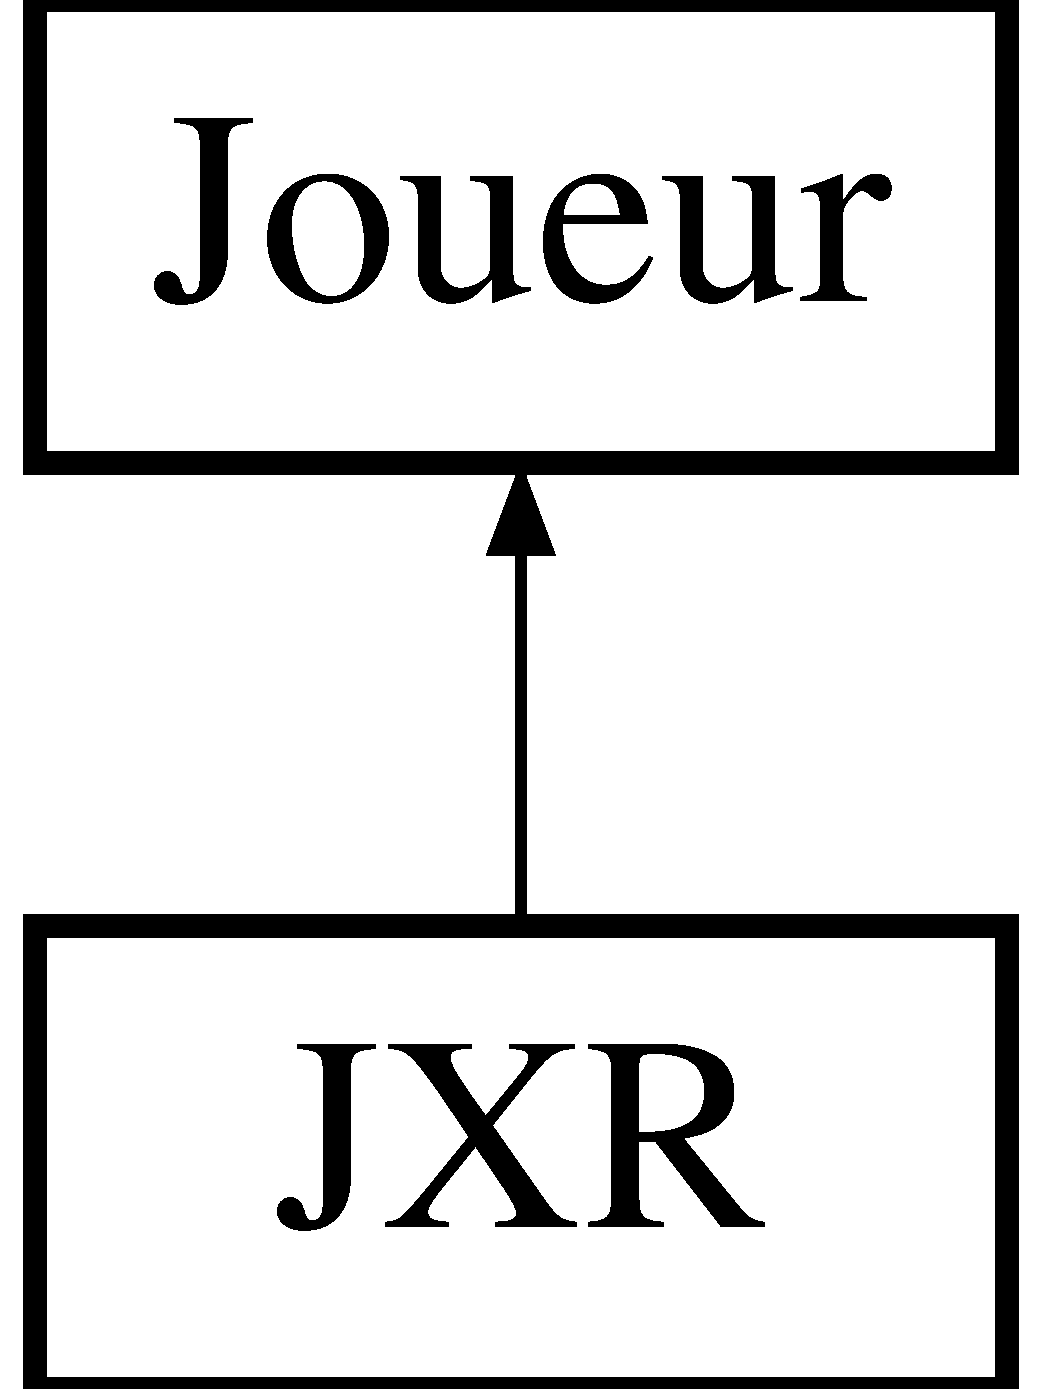
\includegraphics[height=2.000000cm]{class_j_x_r}
\end{center}
\end{figure}
\subsection*{Fonctions membres publiques}
\begin{DoxyCompactItemize}
\item 
\hyperlink{class_j_x_r_aae0980eb175a7241780f7b356bfc225f}{J\-X\-R} (std\-::string nom, std\-::string fichier)
\item 
\hyperlink{class_j_x_r_ab45417fe9d5e2460b6fdfd650692c2e1}{$\sim$\-J\-X\-R} ()
\end{DoxyCompactItemize}


\subsection{Description détaillée}
Fichier \hyperlink{_j_x_r_8hpp}{J\-X\-R.\-hpp} \begin{DoxyAuthor}{Auteur}
Pierre Gaultier \& Theo Dolez 
\end{DoxyAuthor}


\subsection{Documentation des constructeurs et destructeur}
\hypertarget{class_j_x_r_aae0980eb175a7241780f7b356bfc225f}{\index{J\-X\-R@{J\-X\-R}!J\-X\-R@{J\-X\-R}}
\index{J\-X\-R@{J\-X\-R}!JXR@{J\-X\-R}}
\subsubsection[{J\-X\-R}]{\setlength{\rightskip}{0pt plus 5cm}J\-X\-R\-::\-J\-X\-R (
\begin{DoxyParamCaption}
\item[{std\-::string}]{nom, }
\item[{std\-::string}]{fichier}
\end{DoxyParamCaption}
)}}\label{class_j_x_r_aae0980eb175a7241780f7b356bfc225f}
Constructeur qui associe au \hyperlink{class_j_x_r}{J\-X\-R} le comportement du pouvoir du \hyperlink{class_j_x_r}{J\-X\-R}. \hypertarget{class_j_x_r_ab45417fe9d5e2460b6fdfd650692c2e1}{\index{J\-X\-R@{J\-X\-R}!$\sim$\-J\-X\-R@{$\sim$\-J\-X\-R}}
\index{$\sim$\-J\-X\-R@{$\sim$\-J\-X\-R}!JXR@{J\-X\-R}}
\subsubsection[{$\sim$\-J\-X\-R}]{\setlength{\rightskip}{0pt plus 5cm}J\-X\-R\-::$\sim$\-J\-X\-R (
\begin{DoxyParamCaption}
{}
\end{DoxyParamCaption}
)}}\label{class_j_x_r_ab45417fe9d5e2460b6fdfd650692c2e1}
Destructeur 

La documentation de cette classe a été générée à partir des fichiers suivants \-:\begin{DoxyCompactItemize}
\item 
include/\-Modele/\-Joueur/\hyperlink{_j_x_r_8hpp}{J\-X\-R.\-hpp}\item 
src/\-Modele/\-Joueur/\hyperlink{_j_x_r_8cpp}{J\-X\-R.\-cpp}\end{DoxyCompactItemize}

\hypertarget{class_lancement_partie}{\section{Référence de la classe Lancement\-Partie}
\label{class_lancement_partie}\index{Lancement\-Partie@{Lancement\-Partie}}
}


{\ttfamily \#include $<$Lancement\-Partie.\-hpp$>$}

\subsection*{Fonctions membres publiques}
\begin{DoxyCompactItemize}
\item 
\hyperlink{class_lancement_partie_a15c4cd0df7b7b7cd47c26b0f8782adee}{Lancement\-Partie} ()
\item 
\hyperlink{class_lancement_partie_a21f3576e8d380d0fd684d5851787bed0}{$\sim$\-Lancement\-Partie} ()
\item 
void \hyperlink{class_lancement_partie_af84e88126249dfdcbbac1daa329f4ce3}{lancer\-Partie} ()
\end{DoxyCompactItemize}


\subsection{Documentation des constructeurs et destructeur}
\hypertarget{class_lancement_partie_a15c4cd0df7b7b7cd47c26b0f8782adee}{\index{Lancement\-Partie@{Lancement\-Partie}!Lancement\-Partie@{Lancement\-Partie}}
\index{Lancement\-Partie@{Lancement\-Partie}!LancementPartie@{Lancement\-Partie}}
\subsubsection[{Lancement\-Partie}]{\setlength{\rightskip}{0pt plus 5cm}Lancement\-Partie\-::\-Lancement\-Partie (
\begin{DoxyParamCaption}
{}
\end{DoxyParamCaption}
)}}\label{class_lancement_partie_a15c4cd0df7b7b7cd47c26b0f8782adee}
Constructeur. 
\begin{DoxyParams}{Paramètres}
{\em j} & le jeu \\
\hline
\end{DoxyParams}
\hypertarget{class_lancement_partie_a21f3576e8d380d0fd684d5851787bed0}{\index{Lancement\-Partie@{Lancement\-Partie}!$\sim$\-Lancement\-Partie@{$\sim$\-Lancement\-Partie}}
\index{$\sim$\-Lancement\-Partie@{$\sim$\-Lancement\-Partie}!LancementPartie@{Lancement\-Partie}}
\subsubsection[{$\sim$\-Lancement\-Partie}]{\setlength{\rightskip}{0pt plus 5cm}Lancement\-Partie\-::$\sim$\-Lancement\-Partie (
\begin{DoxyParamCaption}
{}
\end{DoxyParamCaption}
)}}\label{class_lancement_partie_a21f3576e8d380d0fd684d5851787bed0}
Destructeur 

\subsection{Documentation des fonctions membres}
\hypertarget{class_lancement_partie_af84e88126249dfdcbbac1daa329f4ce3}{\index{Lancement\-Partie@{Lancement\-Partie}!lancer\-Partie@{lancer\-Partie}}
\index{lancer\-Partie@{lancer\-Partie}!LancementPartie@{Lancement\-Partie}}
\subsubsection[{lancer\-Partie}]{\setlength{\rightskip}{0pt plus 5cm}void Lancement\-Partie\-::lancer\-Partie (
\begin{DoxyParamCaption}
{}
\end{DoxyParamCaption}
)}}\label{class_lancement_partie_af84e88126249dfdcbbac1daa329f4ce3}
Méthode utilisée dans le Main pour lancer une partie (Création des Joueurs, du \hyperlink{class_jeu}{Jeu} ect) 

La documentation de cette classe a été générée à partir des fichiers suivants \-:\begin{DoxyCompactItemize}
\item 
include/\-Controleur/\hyperlink{_lancement_partie_8hpp}{Lancement\-Partie.\-hpp}\item 
src/\-Controleur/\hyperlink{_lancement_partie_8cpp}{Lancement\-Partie.\-cpp}\end{DoxyCompactItemize}

\hypertarget{class_mage}{\section{Référence de la classe Mage}
\label{class_mage}\index{Mage@{Mage}}
}


{\ttfamily \#include $<$Mage.\-hpp$>$}

Graphe d'héritage de Mage\-:\begin{figure}[H]
\begin{center}
\leavevmode
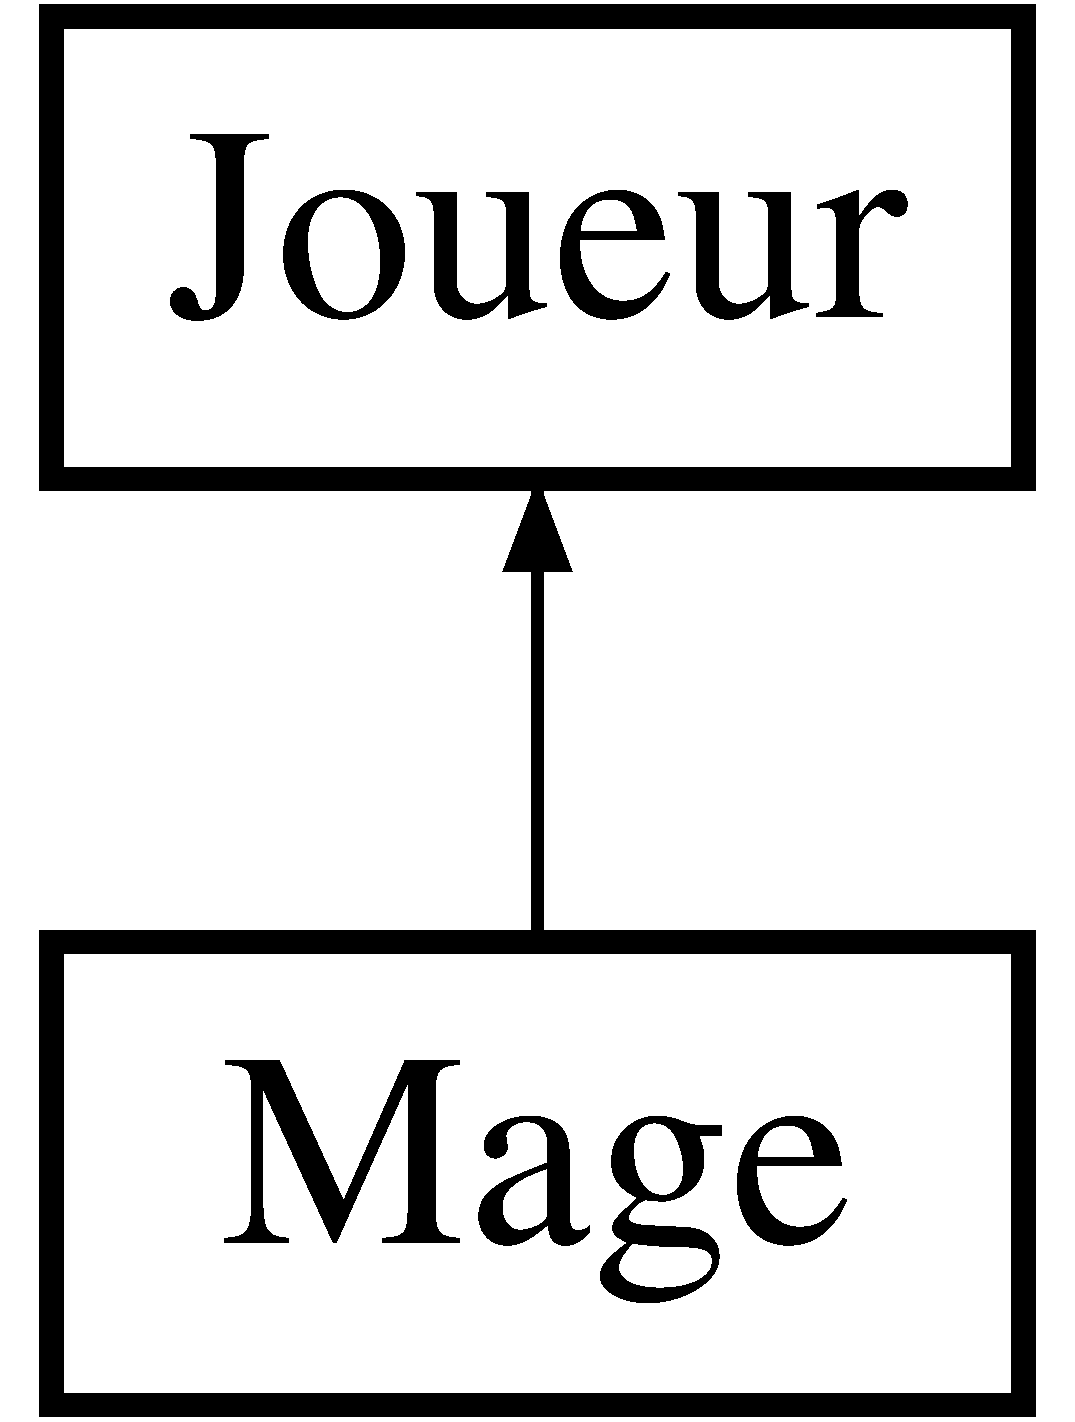
\includegraphics[height=2.000000cm]{class_mage}
\end{center}
\end{figure}
\subsection*{Fonctions membres publiques}
\begin{DoxyCompactItemize}
\item 
\hyperlink{class_mage_afd12913f92aeb59dceb83ad1d6753ae9}{Mage} (std\-::string nom, std\-::string fichier)
\item 
\hyperlink{class_mage_a0a3f693b67379cde4fcf2fa1622211ca}{$\sim$\-Mage} ()
\end{DoxyCompactItemize}


\subsection{Description détaillée}
Fichier \hyperlink{_mage_8hpp}{Mage.\-hpp} \begin{DoxyAuthor}{Auteur}
Pierre Gaultier \& Theo Dolez 
\end{DoxyAuthor}


\subsection{Documentation des constructeurs et destructeur}
\hypertarget{class_mage_afd12913f92aeb59dceb83ad1d6753ae9}{\index{Mage@{Mage}!Mage@{Mage}}
\index{Mage@{Mage}!Mage@{Mage}}
\subsubsection[{Mage}]{\setlength{\rightskip}{0pt plus 5cm}Mage\-::\-Mage (
\begin{DoxyParamCaption}
\item[{std\-::string}]{nom, }
\item[{std\-::string}]{fichier}
\end{DoxyParamCaption}
)}}\label{class_mage_afd12913f92aeb59dceb83ad1d6753ae9}
Constructeur qui associe au \hyperlink{class_mage}{Mage} le comportement du pouvoir du \hyperlink{class_mage}{Mage} \hypertarget{class_mage_a0a3f693b67379cde4fcf2fa1622211ca}{\index{Mage@{Mage}!$\sim$\-Mage@{$\sim$\-Mage}}
\index{$\sim$\-Mage@{$\sim$\-Mage}!Mage@{Mage}}
\subsubsection[{$\sim$\-Mage}]{\setlength{\rightskip}{0pt plus 5cm}Mage\-::$\sim$\-Mage (
\begin{DoxyParamCaption}
{}
\end{DoxyParamCaption}
)}}\label{class_mage_a0a3f693b67379cde4fcf2fa1622211ca}
Destructeur 

La documentation de cette classe a été générée à partir des fichiers suivants \-:\begin{DoxyCompactItemize}
\item 
include/\-Modele/\-Joueur/\hyperlink{_mage_8hpp}{Mage.\-hpp}\item 
src/\-Modele/\-Joueur/\hyperlink{_mage_8cpp}{Mage.\-cpp}\end{DoxyCompactItemize}

\hypertarget{class_observer}{\section{Référence de la classe Observer}
\label{class_observer}\index{Observer@{Observer}}
}


{\ttfamily \#include $<$Observer.\-hpp$>$}

Graphe d'héritage de Observer\-:\begin{figure}[H]
\begin{center}
\leavevmode
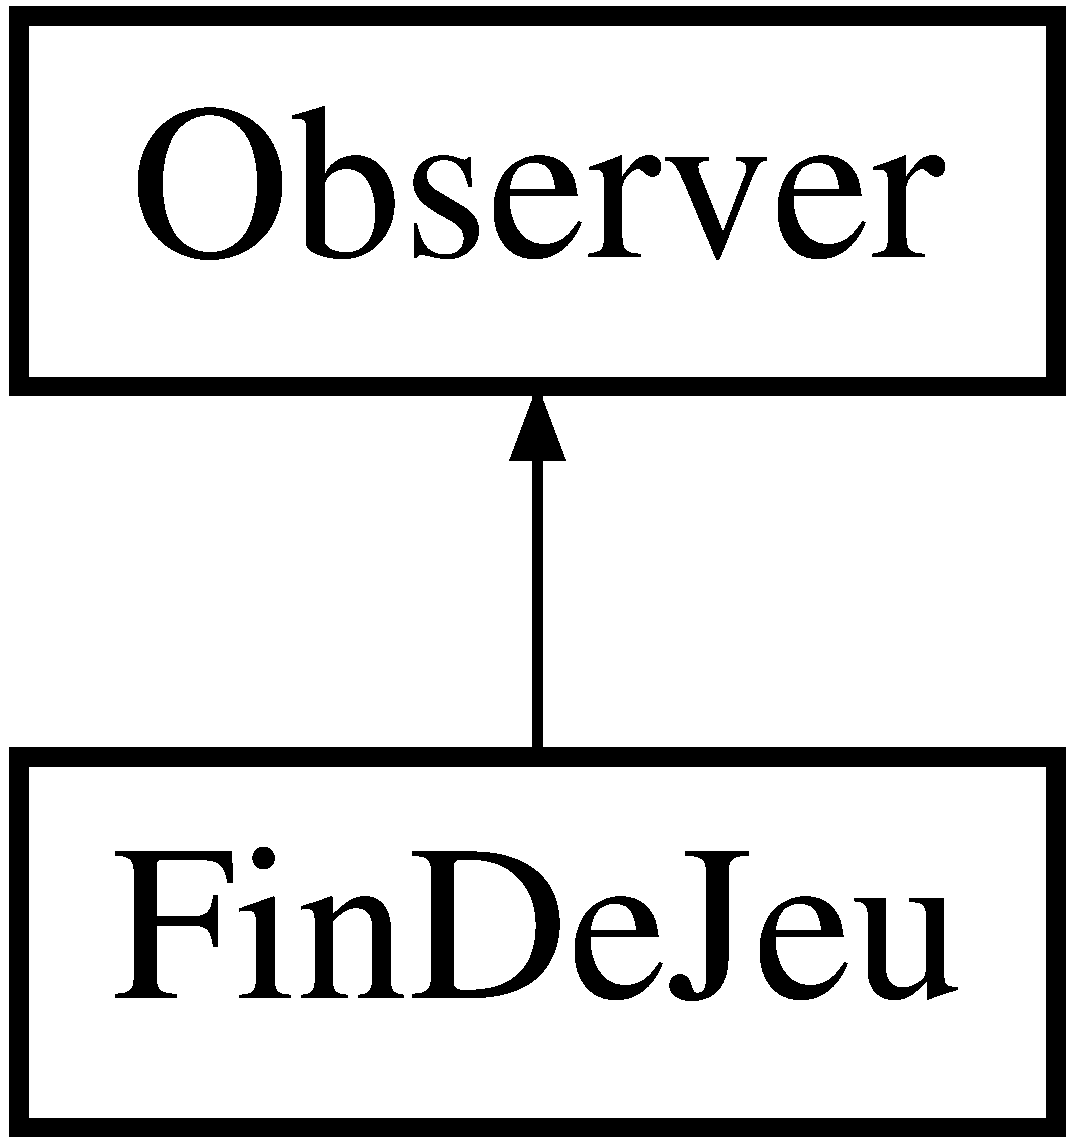
\includegraphics[height=2.000000cm]{class_observer}
\end{center}
\end{figure}
\subsection*{Fonctions membres publiques}
\begin{DoxyCompactItemize}
\item 
virtual \hyperlink{class_observer_afcc6b67be6c386f2f3d2c363aa59cb47}{$\sim$\-Observer} ()
\item 
virtual bool \hyperlink{class_observer_a7930233e1f70d67b3fece5d05e5b6299}{actualiser} ()=0
\end{DoxyCompactItemize}


\subsection{Description détaillée}
Fichier \hyperlink{_observer_8hpp}{Observer.\-hpp} \begin{DoxyAuthor}{Auteur}
Pierre Gaultier \& Theo Dolez 
\end{DoxyAuthor}


\subsection{Documentation des constructeurs et destructeur}
\hypertarget{class_observer_afcc6b67be6c386f2f3d2c363aa59cb47}{\index{Observer@{Observer}!$\sim$\-Observer@{$\sim$\-Observer}}
\index{$\sim$\-Observer@{$\sim$\-Observer}!Observer@{Observer}}
\subsubsection[{$\sim$\-Observer}]{\setlength{\rightskip}{0pt plus 5cm}virtual Observer\-::$\sim$\-Observer (
\begin{DoxyParamCaption}
{}
\end{DoxyParamCaption}
)\hspace{0.3cm}{\ttfamily [inline]}, {\ttfamily [virtual]}}}\label{class_observer_afcc6b67be6c386f2f3d2c363aa59cb47}


\subsection{Documentation des fonctions membres}
\hypertarget{class_observer_a7930233e1f70d67b3fece5d05e5b6299}{\index{Observer@{Observer}!actualiser@{actualiser}}
\index{actualiser@{actualiser}!Observer@{Observer}}
\subsubsection[{actualiser}]{\setlength{\rightskip}{0pt plus 5cm}virtual bool Observer\-::actualiser (
\begin{DoxyParamCaption}
{}
\end{DoxyParamCaption}
)\hspace{0.3cm}{\ttfamily [pure virtual]}}}\label{class_observer_a7930233e1f70d67b3fece5d05e5b6299}


Implémenté dans \hyperlink{class_fin_de_jeu_a79c3fb0a9e367cd3e62da14af840f871}{Fin\-De\-Jeu}.



La documentation de cette classe a été générée à partir du fichier suivant \-:\begin{DoxyCompactItemize}
\item 
include/\-Controleur/\hyperlink{_observer_8hpp}{Observer.\-hpp}\end{DoxyCompactItemize}

\hypertarget{class_pretre}{\section{Référence de la classe Pretre}
\label{class_pretre}\index{Pretre@{Pretre}}
}


{\ttfamily \#include $<$Pretre.\-hpp$>$}

Graphe d'héritage de Pretre\-:\begin{figure}[H]
\begin{center}
\leavevmode
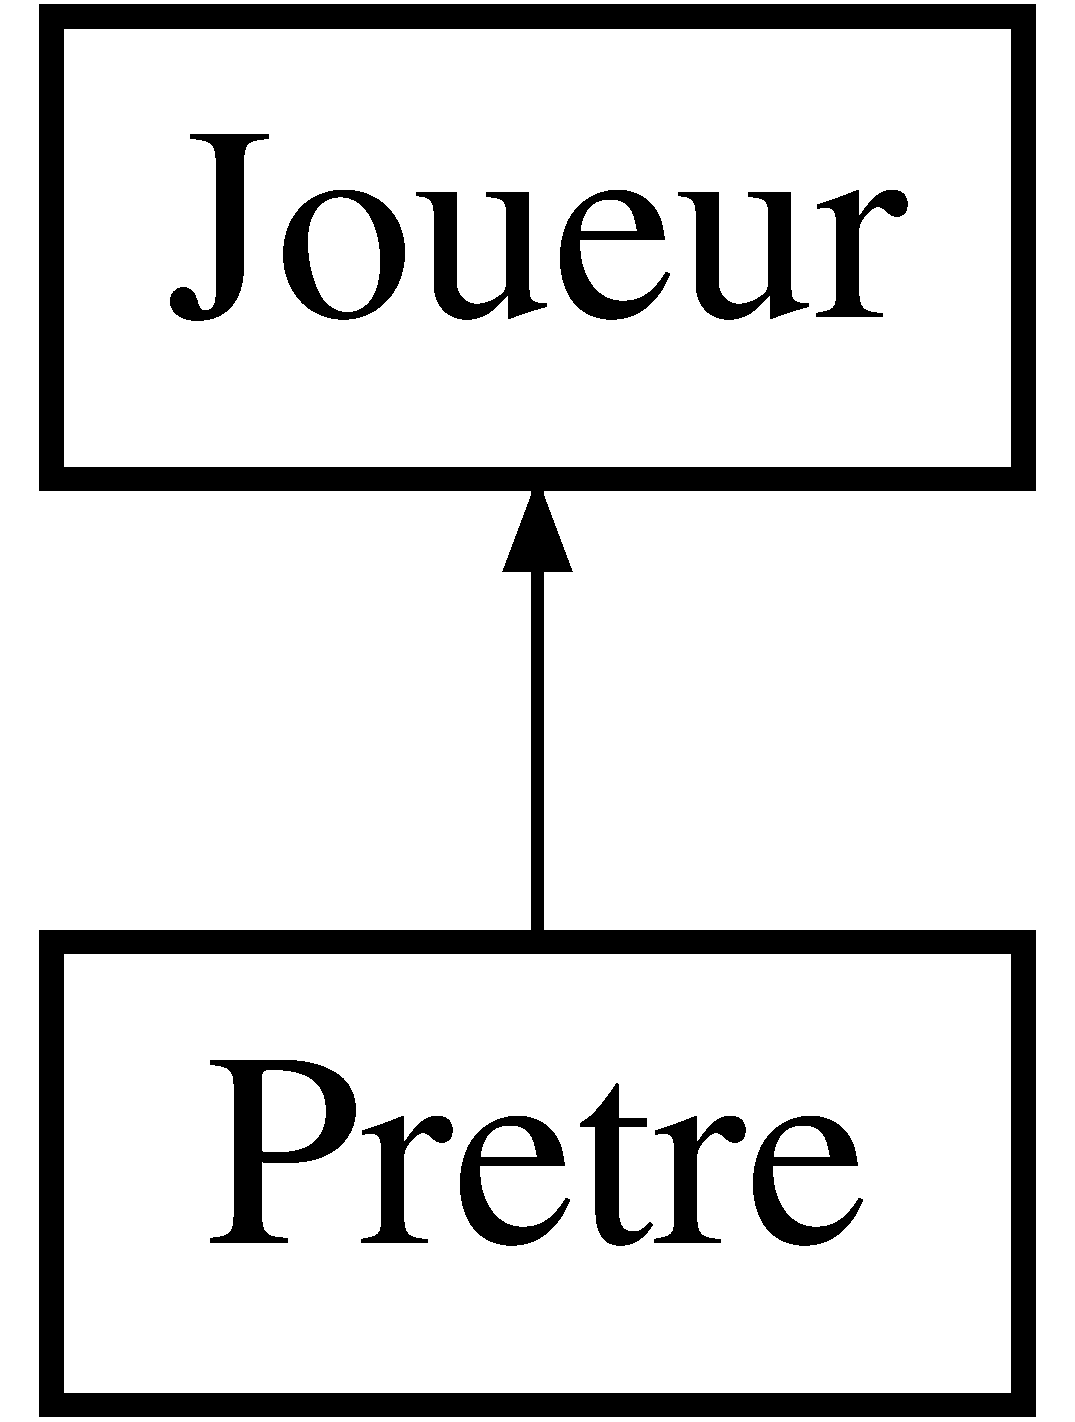
\includegraphics[height=2.000000cm]{class_pretre}
\end{center}
\end{figure}
\subsection*{Fonctions membres publiques}
\begin{DoxyCompactItemize}
\item 
\hyperlink{class_pretre_a05462a17df09bcc3c84cebdcb994b9a5}{Pretre} (std\-::string nom, std\-::string fichier)
\item 
\hyperlink{class_pretre_a9235b9c5f1c57e7d6bb8cba648c43414}{$\sim$\-Pretre} ()
\end{DoxyCompactItemize}


\subsection{Description détaillée}
Fichier \hyperlink{_pretre_8hpp}{Pretre.\-hpp} \begin{DoxyAuthor}{Auteur}
Pierre Gaultier \& Theo Dolez 
\end{DoxyAuthor}


\subsection{Documentation des constructeurs et destructeur}
\hypertarget{class_pretre_a05462a17df09bcc3c84cebdcb994b9a5}{\index{Pretre@{Pretre}!Pretre@{Pretre}}
\index{Pretre@{Pretre}!Pretre@{Pretre}}
\subsubsection[{Pretre}]{\setlength{\rightskip}{0pt plus 5cm}Pretre\-::\-Pretre (
\begin{DoxyParamCaption}
\item[{std\-::string}]{nom, }
\item[{std\-::string}]{fichier}
\end{DoxyParamCaption}
)}}\label{class_pretre_a05462a17df09bcc3c84cebdcb994b9a5}
Constructeur qui associe au \hyperlink{class_pretre}{Pretre} le comportement du pouvoir du \hyperlink{class_pretre}{Pretre} \hypertarget{class_pretre_a9235b9c5f1c57e7d6bb8cba648c43414}{\index{Pretre@{Pretre}!$\sim$\-Pretre@{$\sim$\-Pretre}}
\index{$\sim$\-Pretre@{$\sim$\-Pretre}!Pretre@{Pretre}}
\subsubsection[{$\sim$\-Pretre}]{\setlength{\rightskip}{0pt plus 5cm}Pretre\-::$\sim$\-Pretre (
\begin{DoxyParamCaption}
{}
\end{DoxyParamCaption}
)}}\label{class_pretre_a9235b9c5f1c57e7d6bb8cba648c43414}
Destructeur 

La documentation de cette classe a été générée à partir des fichiers suivants \-:\begin{DoxyCompactItemize}
\item 
include/\-Modele/\-Joueur/\hyperlink{_pretre_8hpp}{Pretre.\-hpp}\item 
src/\-Modele/\-Joueur/\hyperlink{_pretre_8cpp}{Pretre.\-cpp}\end{DoxyCompactItemize}

\hypertarget{class_sujet}{\section{Référence de la classe Sujet}
\label{class_sujet}\index{Sujet@{Sujet}}
}


{\ttfamily \#include $<$Sujet.\-hpp$>$}

Graphe d'héritage de Sujet\-:\begin{figure}[H]
\begin{center}
\leavevmode
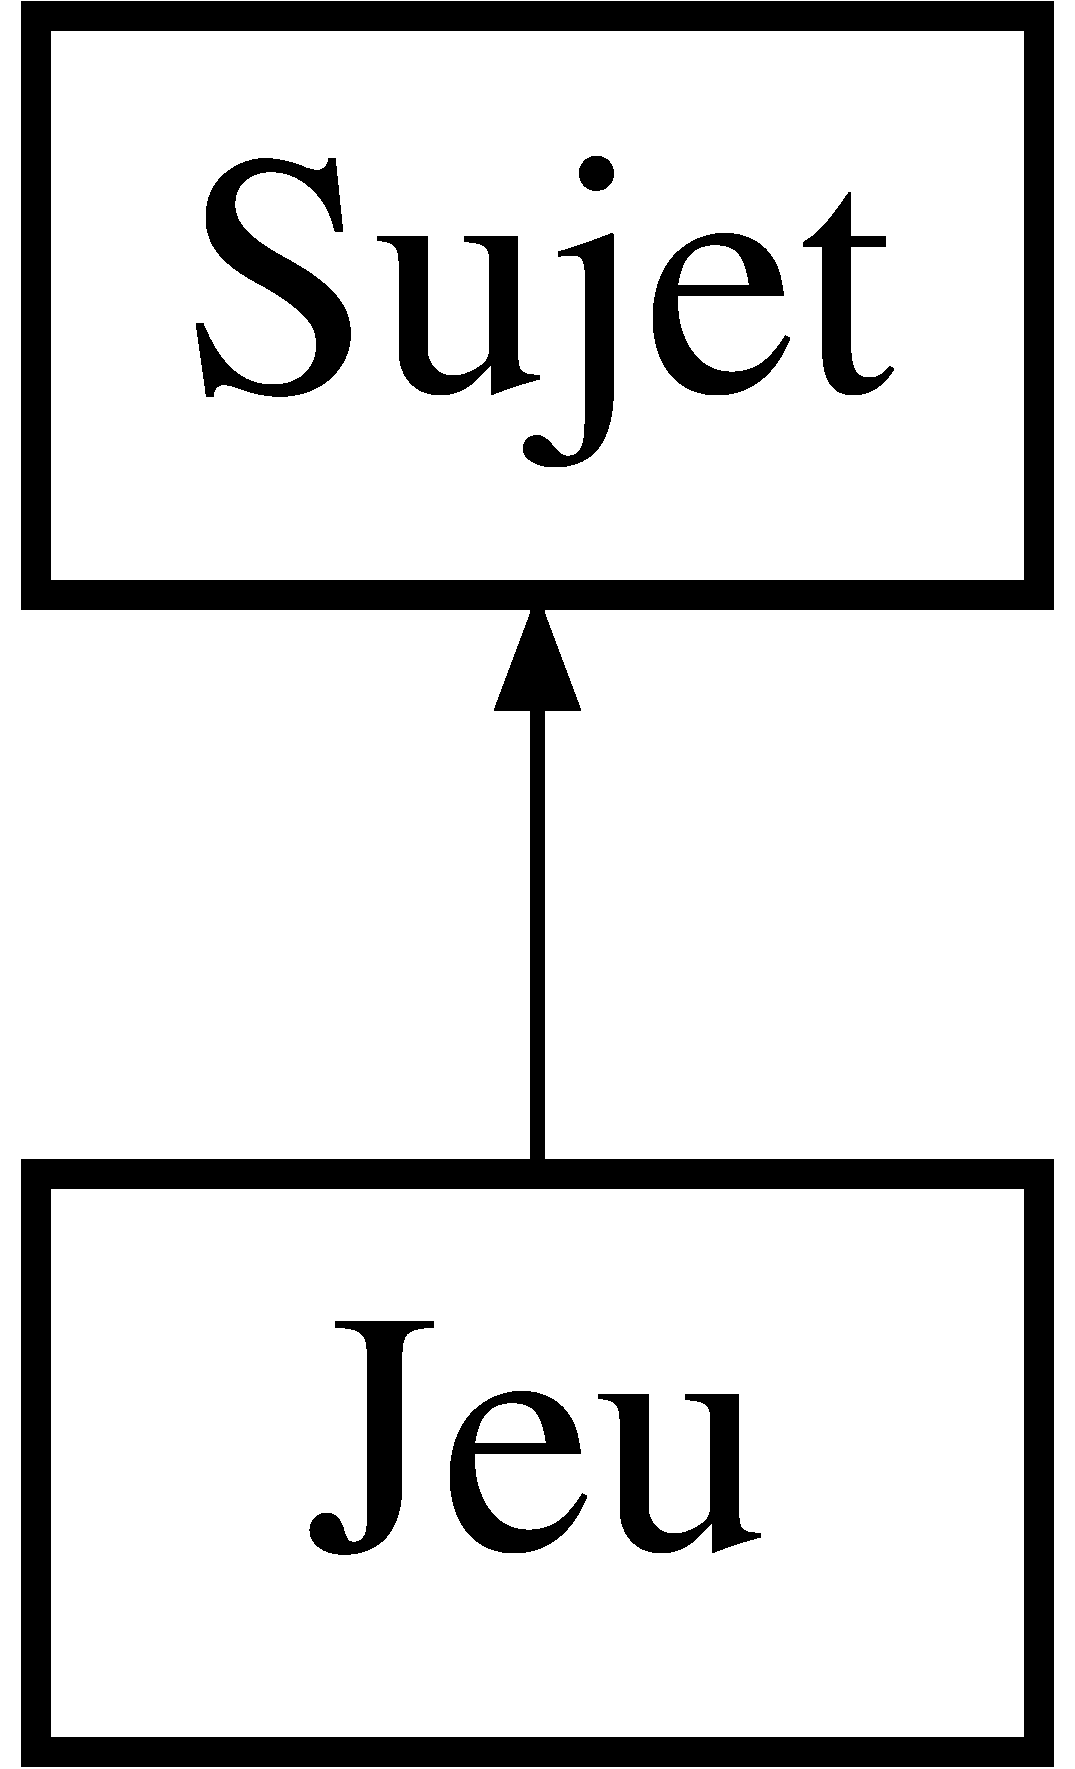
\includegraphics[height=2.000000cm]{class_sujet}
\end{center}
\end{figure}
\subsection*{Fonctions membres publiques}
\begin{DoxyCompactItemize}
\item 
virtual \hyperlink{class_sujet_a0018a7ce3565bfcfc168a993b8dc15f6}{$\sim$\-Sujet} ()
\item 
virtual void \hyperlink{class_sujet_aacd8c7455737c41df8fc5ebbea865745}{enregistrer\-Obs} (\hyperlink{class_observer}{Observer} $\ast$O)=0
\item 
virtual void \hyperlink{class_sujet_a6d121bdc49579675064cfd038b751922}{supprimer\-Obs} (\hyperlink{class_observer}{Observer} $\ast$O)=0
\item 
virtual bool \hyperlink{class_sujet_a210b37440cb4dbb5eff2770a44c14b0d}{notifier\-Obs} ()=0
\end{DoxyCompactItemize}


\subsection{Description détaillée}
Fichier \hyperlink{_sujet_8hpp}{Sujet.\-hpp} \begin{DoxyAuthor}{Auteur}
Pierre Gaultier \& Theo Dolez 
\end{DoxyAuthor}


\subsection{Documentation des constructeurs et destructeur}
\hypertarget{class_sujet_a0018a7ce3565bfcfc168a993b8dc15f6}{\index{Sujet@{Sujet}!$\sim$\-Sujet@{$\sim$\-Sujet}}
\index{$\sim$\-Sujet@{$\sim$\-Sujet}!Sujet@{Sujet}}
\subsubsection[{$\sim$\-Sujet}]{\setlength{\rightskip}{0pt plus 5cm}virtual Sujet\-::$\sim$\-Sujet (
\begin{DoxyParamCaption}
{}
\end{DoxyParamCaption}
)\hspace{0.3cm}{\ttfamily [inline]}, {\ttfamily [virtual]}}}\label{class_sujet_a0018a7ce3565bfcfc168a993b8dc15f6}


\subsection{Documentation des fonctions membres}
\hypertarget{class_sujet_aacd8c7455737c41df8fc5ebbea865745}{\index{Sujet@{Sujet}!enregistrer\-Obs@{enregistrer\-Obs}}
\index{enregistrer\-Obs@{enregistrer\-Obs}!Sujet@{Sujet}}
\subsubsection[{enregistrer\-Obs}]{\setlength{\rightskip}{0pt plus 5cm}virtual void Sujet\-::enregistrer\-Obs (
\begin{DoxyParamCaption}
\item[{{\bf Observer} $\ast$}]{O}
\end{DoxyParamCaption}
)\hspace{0.3cm}{\ttfamily [pure virtual]}}}\label{class_sujet_aacd8c7455737c41df8fc5ebbea865745}


Implémenté dans \hyperlink{class_jeu_a88bf8ed9150f780b02e70decc60a3f02}{Jeu}.

\hypertarget{class_sujet_a210b37440cb4dbb5eff2770a44c14b0d}{\index{Sujet@{Sujet}!notifier\-Obs@{notifier\-Obs}}
\index{notifier\-Obs@{notifier\-Obs}!Sujet@{Sujet}}
\subsubsection[{notifier\-Obs}]{\setlength{\rightskip}{0pt plus 5cm}virtual bool Sujet\-::notifier\-Obs (
\begin{DoxyParamCaption}
{}
\end{DoxyParamCaption}
)\hspace{0.3cm}{\ttfamily [pure virtual]}}}\label{class_sujet_a210b37440cb4dbb5eff2770a44c14b0d}


Implémenté dans \hyperlink{class_jeu_acd9b7a2de81b5ca7d2a5c3b7e5e177e2}{Jeu}.

\hypertarget{class_sujet_a6d121bdc49579675064cfd038b751922}{\index{Sujet@{Sujet}!supprimer\-Obs@{supprimer\-Obs}}
\index{supprimer\-Obs@{supprimer\-Obs}!Sujet@{Sujet}}
\subsubsection[{supprimer\-Obs}]{\setlength{\rightskip}{0pt plus 5cm}virtual void Sujet\-::supprimer\-Obs (
\begin{DoxyParamCaption}
\item[{{\bf Observer} $\ast$}]{O}
\end{DoxyParamCaption}
)\hspace{0.3cm}{\ttfamily [pure virtual]}}}\label{class_sujet_a6d121bdc49579675064cfd038b751922}


Implémenté dans \hyperlink{class_jeu_a8a051ac409a0e53397df3d4578a1e571}{Jeu}.



La documentation de cette classe a été générée à partir du fichier suivant \-:\begin{DoxyCompactItemize}
\item 
include/\-Controleur/\hyperlink{_sujet_8hpp}{Sujet.\-hpp}\end{DoxyCompactItemize}

\hypertarget{class_vue_console}{\section{Référence de la classe Vue\-Console}
\label{class_vue_console}\index{Vue\-Console@{Vue\-Console}}
}


{\ttfamily \#include $<$Vue\-Console.\-hpp$>$}

\subsection*{Fonctions membres publiques}
\begin{DoxyCompactItemize}
\item 
\hyperlink{class_vue_console_a3fc6ba85609459d0919cf9ad4fc1056a}{Vue\-Console} ()
\item 
\hyperlink{class_vue_console_a84554327c266781a3ee5422e1dba674b}{$\sim$\-Vue\-Console} ()
\item 
int \hyperlink{class_vue_console_a8a2212cbdd27511f92f29c222957c80c}{get\-Choix\-Joueur} ()
\item 
string \hyperlink{class_vue_console_a5340da9b0a7fad73fe91b26ec6b20f3b}{get\-Nom\-Joueur} ()
\item 
void \hyperlink{class_vue_console_a0782f21077f7c1be22e798ec445a4d87}{afficher\-Main} (\hyperlink{class_joueur}{Joueur} $\ast$j)
\item 
void \hyperlink{class_vue_console_a44d91e29edaa189252dedd1ee643619d}{afficher\-Choix} ()
\item 
void \hyperlink{class_vue_console_a80c7dcfb3eb9a381b37ba46a7ac366af}{afficher\-Choix\-Debut\-Tour} ()
\item 
void \hyperlink{class_vue_console_aeda02f293126db8b72755d223fe2b0e0}{afficher\-Choix\-No\-Mana} ()
\item 
void \hyperlink{class_vue_console_a52c6059b31bcca4000d94fd2578363b8}{afficher\-Choix\-No\-Attaque} ()
\item 
void \hyperlink{class_vue_console_af38fecfa458f233e81f2beeda1610ec3}{afficher\-Choix\-Double\-No} ()
\item 
void \hyperlink{class_vue_console_a12e8a5246c04cd6ba39fdb29c6b3765a}{afficher\-Choix\-Cv\-C} ()
\item 
void \hyperlink{class_vue_console_ad5941f80c25dd4252db2f803cc9ad7e3}{afficher\-Choix\-Cv\-J} ()
\item 
void \hyperlink{class_vue_console_a956e2949c9c9b1485eb734ba20affcf4}{afficher\-Board} (\hyperlink{class_joueur}{Joueur} $\ast$j)
\item 
void \hyperlink{class_vue_console_af493448120cfaf5c389f741e30bc7b31}{afficher2\-Board} (\hyperlink{class_joueur}{Joueur} $\ast$j1, \hyperlink{class_joueur}{Joueur} $\ast$j2)
\item 
void \hyperlink{class_vue_console_ad450cc024c4c7797c18f399b0f4c321c}{afficher\-Personnage} (\hyperlink{class_joueur}{Joueur} $\ast$j)
\item 
void \hyperlink{class_vue_console_ae015f7453d65bb89abef4793addc18ca}{afficher\-Personnage\-Autre} (\hyperlink{class_joueur}{Joueur} $\ast$j)
\item 
void \hyperlink{class_vue_console_a64ad6e083263f0fadef29b98207cb2aa}{afficher\-Debut\-Tour} (\hyperlink{class_joueur}{Joueur} $\ast$j)
\item 
void \hyperlink{class_vue_console_ada125e06218ee32a5dbacc526e28a84c}{afficher\-Fin\-Tour} ()
\item 
void \hyperlink{class_vue_console_a0f4cab13a73ac5c80881276687a506aa}{afficher\-Jouer\-Carte} ()
\item 
void \hyperlink{class_vue_console_a9f1b65a45e8e3da31ae35fa6c4d53dce}{afficher\-Pdmn\-Restant} (int i)
\item 
void \hyperlink{class_vue_console_a2b469256d2776aa6e01ebc4bd393c2a3}{afficher\-Pas\-Assez\-De\-Mana} ()
\item 
void \hyperlink{class_vue_console_a525f3eacad711387238b37a9b64c5406}{afficher\-Choix\-Pouvoir\-Mage} ()
\item 
void \hyperlink{class_vue_console_ac1e6d5da6ce2c352d10c665d79c616d0}{afficher\-Choix\-Pouvoir\-Pretre} ()
\item 
void \hyperlink{class_vue_console_a884aeedbd65ebe011b86f42d6ae5db04}{afficher\-Choix\-Pouvoir\-Induction} ()
\item 
void \hyperlink{class_vue_console_ad55bf2d0d6397204cccfb488aad39c4e}{afficher\-Choix\-Carte} ()
\item 
void \hyperlink{class_vue_console_a2f811063bc7f2dcac117d7a49df36931}{afficher\-Erreur\-Choix} ()
\item 
void \hyperlink{class_vue_console_a9e339ac2f7b3f337d4a2951db490815b}{afficher\-Pas\-De\-Carte\-Adverse} ()
\item 
void \hyperlink{class_vue_console_a4a9f289f010e643b5e8a004f3fe539ac}{afficher\-Pas\-De\-Carte\-Board} ()
\item 
void \hyperlink{class_vue_console_a1e9faf3a19588ff0f659dfff4cfcff09}{afficher\-Intro} ()
\item 
void \hyperlink{class_vue_console_a945e04f68fb5a0089e35b1b688001b87}{afficher\-Fin\-Intro} ()
\end{DoxyCompactItemize}


\subsection{Documentation des constructeurs et destructeur}
\hypertarget{class_vue_console_a3fc6ba85609459d0919cf9ad4fc1056a}{\index{Vue\-Console@{Vue\-Console}!Vue\-Console@{Vue\-Console}}
\index{Vue\-Console@{Vue\-Console}!VueConsole@{Vue\-Console}}
\subsubsection[{Vue\-Console}]{\setlength{\rightskip}{0pt plus 5cm}Vue\-Console\-::\-Vue\-Console (
\begin{DoxyParamCaption}
{}
\end{DoxyParamCaption}
)}}\label{class_vue_console_a3fc6ba85609459d0919cf9ad4fc1056a}
Constructeur \hypertarget{class_vue_console_a84554327c266781a3ee5422e1dba674b}{\index{Vue\-Console@{Vue\-Console}!$\sim$\-Vue\-Console@{$\sim$\-Vue\-Console}}
\index{$\sim$\-Vue\-Console@{$\sim$\-Vue\-Console}!VueConsole@{Vue\-Console}}
\subsubsection[{$\sim$\-Vue\-Console}]{\setlength{\rightskip}{0pt plus 5cm}Vue\-Console\-::$\sim$\-Vue\-Console (
\begin{DoxyParamCaption}
{}
\end{DoxyParamCaption}
)}}\label{class_vue_console_a84554327c266781a3ee5422e1dba674b}
Destructeur 

\subsection{Documentation des fonctions membres}
\hypertarget{class_vue_console_af493448120cfaf5c389f741e30bc7b31}{\index{Vue\-Console@{Vue\-Console}!afficher2\-Board@{afficher2\-Board}}
\index{afficher2\-Board@{afficher2\-Board}!VueConsole@{Vue\-Console}}
\subsubsection[{afficher2\-Board}]{\setlength{\rightskip}{0pt plus 5cm}void Vue\-Console\-::afficher2\-Board (
\begin{DoxyParamCaption}
\item[{{\bf Joueur} $\ast$}]{j1, }
\item[{{\bf Joueur} $\ast$}]{j2}
\end{DoxyParamCaption}
)}}\label{class_vue_console_af493448120cfaf5c389f741e30bc7b31}
Affiche le Board des 2 joueurs. 
\begin{DoxyParams}{Paramètres}
{\em j1} & Le premier \hyperlink{class_joueur}{Joueur}. \\
\hline
{\em j2} & Le deuxième \hyperlink{class_joueur}{Joueur}. \\
\hline
\end{DoxyParams}
\hypertarget{class_vue_console_a956e2949c9c9b1485eb734ba20affcf4}{\index{Vue\-Console@{Vue\-Console}!afficher\-Board@{afficher\-Board}}
\index{afficher\-Board@{afficher\-Board}!VueConsole@{Vue\-Console}}
\subsubsection[{afficher\-Board}]{\setlength{\rightskip}{0pt plus 5cm}void Vue\-Console\-::afficher\-Board (
\begin{DoxyParamCaption}
\item[{{\bf Joueur} $\ast$}]{j}
\end{DoxyParamCaption}
)}}\label{class_vue_console_a956e2949c9c9b1485eb734ba20affcf4}
Affiche le Board du \hyperlink{class_joueur}{Joueur} entré en paramètre. 
\begin{DoxyParams}{Paramètres}
{\em j} & Le joueur. \\
\hline
\end{DoxyParams}
\hypertarget{class_vue_console_a44d91e29edaa189252dedd1ee643619d}{\index{Vue\-Console@{Vue\-Console}!afficher\-Choix@{afficher\-Choix}}
\index{afficher\-Choix@{afficher\-Choix}!VueConsole@{Vue\-Console}}
\subsubsection[{afficher\-Choix}]{\setlength{\rightskip}{0pt plus 5cm}void Vue\-Console\-::afficher\-Choix (
\begin{DoxyParamCaption}
{}
\end{DoxyParamCaption}
)}}\label{class_vue_console_a44d91e29edaa189252dedd1ee643619d}
\hypertarget{class_vue_console_ad55bf2d0d6397204cccfb488aad39c4e}{\index{Vue\-Console@{Vue\-Console}!afficher\-Choix\-Carte@{afficher\-Choix\-Carte}}
\index{afficher\-Choix\-Carte@{afficher\-Choix\-Carte}!VueConsole@{Vue\-Console}}
\subsubsection[{afficher\-Choix\-Carte}]{\setlength{\rightskip}{0pt plus 5cm}void Vue\-Console\-::afficher\-Choix\-Carte (
\begin{DoxyParamCaption}
{}
\end{DoxyParamCaption}
)}}\label{class_vue_console_ad55bf2d0d6397204cccfb488aad39c4e}
Affiche \char`\"{}\-Veuillez indiquer le numéro de la carte cible. \char`\"{}. \hypertarget{class_vue_console_a12e8a5246c04cd6ba39fdb29c6b3765a}{\index{Vue\-Console@{Vue\-Console}!afficher\-Choix\-Cv\-C@{afficher\-Choix\-Cv\-C}}
\index{afficher\-Choix\-Cv\-C@{afficher\-Choix\-Cv\-C}!VueConsole@{Vue\-Console}}
\subsubsection[{afficher\-Choix\-Cv\-C}]{\setlength{\rightskip}{0pt plus 5cm}void Vue\-Console\-::afficher\-Choix\-Cv\-C (
\begin{DoxyParamCaption}
{}
\end{DoxyParamCaption}
)}}\label{class_vue_console_a12e8a5246c04cd6ba39fdb29c6b3765a}
Affiche \char`\"{}\-Entrez le numéro de votre Carte, appuyez sur Entrée, puis faites de même avec la Carte de l'adversaire\char`\"{}; \hypertarget{class_vue_console_ad5941f80c25dd4252db2f803cc9ad7e3}{\index{Vue\-Console@{Vue\-Console}!afficher\-Choix\-Cv\-J@{afficher\-Choix\-Cv\-J}}
\index{afficher\-Choix\-Cv\-J@{afficher\-Choix\-Cv\-J}!VueConsole@{Vue\-Console}}
\subsubsection[{afficher\-Choix\-Cv\-J}]{\setlength{\rightskip}{0pt plus 5cm}void Vue\-Console\-::afficher\-Choix\-Cv\-J (
\begin{DoxyParamCaption}
{}
\end{DoxyParamCaption}
)}}\label{class_vue_console_ad5941f80c25dd4252db2f803cc9ad7e3}
Affiche \char`\"{}\-Entrez le numéro de votre Carte, appuyez sur Entrée\char`\"{}. \hypertarget{class_vue_console_a80c7dcfb3eb9a381b37ba46a7ac366af}{\index{Vue\-Console@{Vue\-Console}!afficher\-Choix\-Debut\-Tour@{afficher\-Choix\-Debut\-Tour}}
\index{afficher\-Choix\-Debut\-Tour@{afficher\-Choix\-Debut\-Tour}!VueConsole@{Vue\-Console}}
\subsubsection[{afficher\-Choix\-Debut\-Tour}]{\setlength{\rightskip}{0pt plus 5cm}void Vue\-Console\-::afficher\-Choix\-Debut\-Tour (
\begin{DoxyParamCaption}
{}
\end{DoxyParamCaption}
)}}\label{class_vue_console_a80c7dcfb3eb9a381b37ba46a7ac366af}
Affiche les choix du \hyperlink{class_joueur}{Joueur} pour l'état Debut Tour. \hypertarget{class_vue_console_af38fecfa458f233e81f2beeda1610ec3}{\index{Vue\-Console@{Vue\-Console}!afficher\-Choix\-Double\-No@{afficher\-Choix\-Double\-No}}
\index{afficher\-Choix\-Double\-No@{afficher\-Choix\-Double\-No}!VueConsole@{Vue\-Console}}
\subsubsection[{afficher\-Choix\-Double\-No}]{\setlength{\rightskip}{0pt plus 5cm}void Vue\-Console\-::afficher\-Choix\-Double\-No (
\begin{DoxyParamCaption}
{}
\end{DoxyParamCaption}
)}}\label{class_vue_console_af38fecfa458f233e81f2beeda1610ec3}
Affiche les choix du \hyperlink{class_joueur}{Joueur} pour l'état Double No. \hypertarget{class_vue_console_a52c6059b31bcca4000d94fd2578363b8}{\index{Vue\-Console@{Vue\-Console}!afficher\-Choix\-No\-Attaque@{afficher\-Choix\-No\-Attaque}}
\index{afficher\-Choix\-No\-Attaque@{afficher\-Choix\-No\-Attaque}!VueConsole@{Vue\-Console}}
\subsubsection[{afficher\-Choix\-No\-Attaque}]{\setlength{\rightskip}{0pt plus 5cm}void Vue\-Console\-::afficher\-Choix\-No\-Attaque (
\begin{DoxyParamCaption}
{}
\end{DoxyParamCaption}
)}}\label{class_vue_console_a52c6059b31bcca4000d94fd2578363b8}
Affiche les choix du \hyperlink{class_joueur}{Joueur} pour l'état No Attaque. \hypertarget{class_vue_console_aeda02f293126db8b72755d223fe2b0e0}{\index{Vue\-Console@{Vue\-Console}!afficher\-Choix\-No\-Mana@{afficher\-Choix\-No\-Mana}}
\index{afficher\-Choix\-No\-Mana@{afficher\-Choix\-No\-Mana}!VueConsole@{Vue\-Console}}
\subsubsection[{afficher\-Choix\-No\-Mana}]{\setlength{\rightskip}{0pt plus 5cm}void Vue\-Console\-::afficher\-Choix\-No\-Mana (
\begin{DoxyParamCaption}
{}
\end{DoxyParamCaption}
)}}\label{class_vue_console_aeda02f293126db8b72755d223fe2b0e0}
Affiche les choix du \hyperlink{class_joueur}{Joueur} pour l'état No Mana. \hypertarget{class_vue_console_a884aeedbd65ebe011b86f42d6ae5db04}{\index{Vue\-Console@{Vue\-Console}!afficher\-Choix\-Pouvoir\-Induction@{afficher\-Choix\-Pouvoir\-Induction}}
\index{afficher\-Choix\-Pouvoir\-Induction@{afficher\-Choix\-Pouvoir\-Induction}!VueConsole@{Vue\-Console}}
\subsubsection[{afficher\-Choix\-Pouvoir\-Induction}]{\setlength{\rightskip}{0pt plus 5cm}void Vue\-Console\-::afficher\-Choix\-Pouvoir\-Induction (
\begin{DoxyParamCaption}
{}
\end{DoxyParamCaption}
)}}\label{class_vue_console_a884aeedbd65ebe011b86f42d6ae5db04}
Affiche \char`\"{}\-Choisissez la carte adverse qui subira L'\-I\-N\-D\-U\-C\-T\-I\-O\-N N\-O\-E\-U\-T\-H\-E\-R\-I\-E\-N\-N\-E ! M\-U\-A\-H\-A\-H\-A\-H\-A\-H\-H\-A!\char`\"{}. \hypertarget{class_vue_console_a525f3eacad711387238b37a9b64c5406}{\index{Vue\-Console@{Vue\-Console}!afficher\-Choix\-Pouvoir\-Mage@{afficher\-Choix\-Pouvoir\-Mage}}
\index{afficher\-Choix\-Pouvoir\-Mage@{afficher\-Choix\-Pouvoir\-Mage}!VueConsole@{Vue\-Console}}
\subsubsection[{afficher\-Choix\-Pouvoir\-Mage}]{\setlength{\rightskip}{0pt plus 5cm}void Vue\-Console\-::afficher\-Choix\-Pouvoir\-Mage (
\begin{DoxyParamCaption}
{}
\end{DoxyParamCaption}
)}}\label{class_vue_console_a525f3eacad711387238b37a9b64c5406}
Affiche les choix pour le pouvoir du \hyperlink{class_mage}{Mage}. \hypertarget{class_vue_console_ac1e6d5da6ce2c352d10c665d79c616d0}{\index{Vue\-Console@{Vue\-Console}!afficher\-Choix\-Pouvoir\-Pretre@{afficher\-Choix\-Pouvoir\-Pretre}}
\index{afficher\-Choix\-Pouvoir\-Pretre@{afficher\-Choix\-Pouvoir\-Pretre}!VueConsole@{Vue\-Console}}
\subsubsection[{afficher\-Choix\-Pouvoir\-Pretre}]{\setlength{\rightskip}{0pt plus 5cm}void Vue\-Console\-::afficher\-Choix\-Pouvoir\-Pretre (
\begin{DoxyParamCaption}
{}
\end{DoxyParamCaption}
)}}\label{class_vue_console_ac1e6d5da6ce2c352d10c665d79c616d0}
Affiche les choix pour le pouvoir du \hyperlink{class_pretre}{Pretre}. \hypertarget{class_vue_console_a64ad6e083263f0fadef29b98207cb2aa}{\index{Vue\-Console@{Vue\-Console}!afficher\-Debut\-Tour@{afficher\-Debut\-Tour}}
\index{afficher\-Debut\-Tour@{afficher\-Debut\-Tour}!VueConsole@{Vue\-Console}}
\subsubsection[{afficher\-Debut\-Tour}]{\setlength{\rightskip}{0pt plus 5cm}void Vue\-Console\-::afficher\-Debut\-Tour (
\begin{DoxyParamCaption}
\item[{{\bf Joueur} $\ast$}]{j}
\end{DoxyParamCaption}
)}}\label{class_vue_console_a64ad6e083263f0fadef29b98207cb2aa}
Affiche les informations du \hyperlink{class_joueur}{Joueur} entré en paramètre au début de son tour. 
\begin{DoxyParams}{Paramètres}
{\em j} & Le joueur. \\
\hline
\end{DoxyParams}
\hypertarget{class_vue_console_a2f811063bc7f2dcac117d7a49df36931}{\index{Vue\-Console@{Vue\-Console}!afficher\-Erreur\-Choix@{afficher\-Erreur\-Choix}}
\index{afficher\-Erreur\-Choix@{afficher\-Erreur\-Choix}!VueConsole@{Vue\-Console}}
\subsubsection[{afficher\-Erreur\-Choix}]{\setlength{\rightskip}{0pt plus 5cm}void Vue\-Console\-::afficher\-Erreur\-Choix (
\begin{DoxyParamCaption}
{}
\end{DoxyParamCaption}
)}}\label{class_vue_console_a2f811063bc7f2dcac117d7a49df36931}
Affiche \char`\"{}\-Veuillez entrer un choix valide ! \-:)\char`\"{}. \hypertarget{class_vue_console_a945e04f68fb5a0089e35b1b688001b87}{\index{Vue\-Console@{Vue\-Console}!afficher\-Fin\-Intro@{afficher\-Fin\-Intro}}
\index{afficher\-Fin\-Intro@{afficher\-Fin\-Intro}!VueConsole@{Vue\-Console}}
\subsubsection[{afficher\-Fin\-Intro}]{\setlength{\rightskip}{0pt plus 5cm}void Vue\-Console\-::afficher\-Fin\-Intro (
\begin{DoxyParamCaption}
{}
\end{DoxyParamCaption}
)}}\label{class_vue_console_a945e04f68fb5a0089e35b1b688001b87}
Affiche la fin de l'intro du jeu. \hypertarget{class_vue_console_ada125e06218ee32a5dbacc526e28a84c}{\index{Vue\-Console@{Vue\-Console}!afficher\-Fin\-Tour@{afficher\-Fin\-Tour}}
\index{afficher\-Fin\-Tour@{afficher\-Fin\-Tour}!VueConsole@{Vue\-Console}}
\subsubsection[{afficher\-Fin\-Tour}]{\setlength{\rightskip}{0pt plus 5cm}void Vue\-Console\-::afficher\-Fin\-Tour (
\begin{DoxyParamCaption}
{}
\end{DoxyParamCaption}
)}}\label{class_vue_console_ada125e06218ee32a5dbacc526e28a84c}
Affiche \char`\"{}\-Fin du Tour\char`\"{}. \hypertarget{class_vue_console_a1e9faf3a19588ff0f659dfff4cfcff09}{\index{Vue\-Console@{Vue\-Console}!afficher\-Intro@{afficher\-Intro}}
\index{afficher\-Intro@{afficher\-Intro}!VueConsole@{Vue\-Console}}
\subsubsection[{afficher\-Intro}]{\setlength{\rightskip}{0pt plus 5cm}void Vue\-Console\-::afficher\-Intro (
\begin{DoxyParamCaption}
{}
\end{DoxyParamCaption}
)}}\label{class_vue_console_a1e9faf3a19588ff0f659dfff4cfcff09}
Affiche l'intro du jeu. \hypertarget{class_vue_console_a0f4cab13a73ac5c80881276687a506aa}{\index{Vue\-Console@{Vue\-Console}!afficher\-Jouer\-Carte@{afficher\-Jouer\-Carte}}
\index{afficher\-Jouer\-Carte@{afficher\-Jouer\-Carte}!VueConsole@{Vue\-Console}}
\subsubsection[{afficher\-Jouer\-Carte}]{\setlength{\rightskip}{0pt plus 5cm}void Vue\-Console\-::afficher\-Jouer\-Carte (
\begin{DoxyParamCaption}
{}
\end{DoxyParamCaption}
)}}\label{class_vue_console_a0f4cab13a73ac5c80881276687a506aa}
Affiche \char`\"{}\-Quelle carte voulez-\/vous jouer ?\char`\"{}. \hypertarget{class_vue_console_a0782f21077f7c1be22e798ec445a4d87}{\index{Vue\-Console@{Vue\-Console}!afficher\-Main@{afficher\-Main}}
\index{afficher\-Main@{afficher\-Main}!VueConsole@{Vue\-Console}}
\subsubsection[{afficher\-Main}]{\setlength{\rightskip}{0pt plus 5cm}void Vue\-Console\-::afficher\-Main (
\begin{DoxyParamCaption}
\item[{{\bf Joueur} $\ast$}]{j}
\end{DoxyParamCaption}
)}}\label{class_vue_console_a0782f21077f7c1be22e798ec445a4d87}
Affiche la main du \hyperlink{class_joueur}{Joueur}. \hypertarget{class_vue_console_a2b469256d2776aa6e01ebc4bd393c2a3}{\index{Vue\-Console@{Vue\-Console}!afficher\-Pas\-Assez\-De\-Mana@{afficher\-Pas\-Assez\-De\-Mana}}
\index{afficher\-Pas\-Assez\-De\-Mana@{afficher\-Pas\-Assez\-De\-Mana}!VueConsole@{Vue\-Console}}
\subsubsection[{afficher\-Pas\-Assez\-De\-Mana}]{\setlength{\rightskip}{0pt plus 5cm}void Vue\-Console\-::afficher\-Pas\-Assez\-De\-Mana (
\begin{DoxyParamCaption}
{}
\end{DoxyParamCaption}
)}}\label{class_vue_console_a2b469256d2776aa6e01ebc4bd393c2a3}
Affiche \char`\"{}\-Pas assez de Mana!\char`\"{}. \hypertarget{class_vue_console_a9e339ac2f7b3f337d4a2951db490815b}{\index{Vue\-Console@{Vue\-Console}!afficher\-Pas\-De\-Carte\-Adverse@{afficher\-Pas\-De\-Carte\-Adverse}}
\index{afficher\-Pas\-De\-Carte\-Adverse@{afficher\-Pas\-De\-Carte\-Adverse}!VueConsole@{Vue\-Console}}
\subsubsection[{afficher\-Pas\-De\-Carte\-Adverse}]{\setlength{\rightskip}{0pt plus 5cm}void Vue\-Console\-::afficher\-Pas\-De\-Carte\-Adverse (
\begin{DoxyParamCaption}
{}
\end{DoxyParamCaption}
)}}\label{class_vue_console_a9e339ac2f7b3f337d4a2951db490815b}
Affiche \char`\"{}\-Il n'y a pas de serviteurs sur le board ennemi ! \char`\"{}. \hypertarget{class_vue_console_a4a9f289f010e643b5e8a004f3fe539ac}{\index{Vue\-Console@{Vue\-Console}!afficher\-Pas\-De\-Carte\-Board@{afficher\-Pas\-De\-Carte\-Board}}
\index{afficher\-Pas\-De\-Carte\-Board@{afficher\-Pas\-De\-Carte\-Board}!VueConsole@{Vue\-Console}}
\subsubsection[{afficher\-Pas\-De\-Carte\-Board}]{\setlength{\rightskip}{0pt plus 5cm}void Vue\-Console\-::afficher\-Pas\-De\-Carte\-Board (
\begin{DoxyParamCaption}
{}
\end{DoxyParamCaption}
)}}\label{class_vue_console_a4a9f289f010e643b5e8a004f3fe539ac}
Affiche \char`\"{}\-Il n'y a pas de serviteurs sur le board ennemi ! \char`\"{}. \hypertarget{class_vue_console_a9f1b65a45e8e3da31ae35fa6c4d53dce}{\index{Vue\-Console@{Vue\-Console}!afficher\-Pdmn\-Restant@{afficher\-Pdmn\-Restant}}
\index{afficher\-Pdmn\-Restant@{afficher\-Pdmn\-Restant}!VueConsole@{Vue\-Console}}
\subsubsection[{afficher\-Pdmn\-Restant}]{\setlength{\rightskip}{0pt plus 5cm}void Vue\-Console\-::afficher\-Pdmn\-Restant (
\begin{DoxyParamCaption}
\item[{int}]{i}
\end{DoxyParamCaption}
)}}\label{class_vue_console_a9f1b65a45e8e3da31ae35fa6c4d53dce}
Affiche les points de mana restant du \hyperlink{class_joueur}{Joueur} (valeur entrée en paramètre) 
\begin{DoxyParams}{Paramètres}
{\em i} & Le nombre de Pts de Mana restant. \\
\hline
\end{DoxyParams}
\hypertarget{class_vue_console_ad450cc024c4c7797c18f399b0f4c321c}{\index{Vue\-Console@{Vue\-Console}!afficher\-Personnage@{afficher\-Personnage}}
\index{afficher\-Personnage@{afficher\-Personnage}!VueConsole@{Vue\-Console}}
\subsubsection[{afficher\-Personnage}]{\setlength{\rightskip}{0pt plus 5cm}void Vue\-Console\-::afficher\-Personnage (
\begin{DoxyParamCaption}
\item[{{\bf Joueur} $\ast$}]{j}
\end{DoxyParamCaption}
)}}\label{class_vue_console_ad450cc024c4c7797c18f399b0f4c321c}
Affiche les informations relatives à un \hyperlink{class_joueur}{Joueur} j entré en paramètre. 
\begin{DoxyParams}{Paramètres}
{\em j} & Le \hyperlink{class_joueur}{Joueur}. \\
\hline
\end{DoxyParams}
\hypertarget{class_vue_console_ae015f7453d65bb89abef4793addc18ca}{\index{Vue\-Console@{Vue\-Console}!afficher\-Personnage\-Autre@{afficher\-Personnage\-Autre}}
\index{afficher\-Personnage\-Autre@{afficher\-Personnage\-Autre}!VueConsole@{Vue\-Console}}
\subsubsection[{afficher\-Personnage\-Autre}]{\setlength{\rightskip}{0pt plus 5cm}void Vue\-Console\-::afficher\-Personnage\-Autre (
\begin{DoxyParamCaption}
\item[{{\bf Joueur} $\ast$}]{j}
\end{DoxyParamCaption}
)}}\label{class_vue_console_ae015f7453d65bb89abef4793addc18ca}
Affiche les informations relatives à un \hyperlink{class_joueur}{Joueur} j entré en paramètre. (destiné pour l'adversaire) 
\begin{DoxyParams}{Paramètres}
{\em j} & Le \hyperlink{class_joueur}{Joueur}. \\
\hline
\end{DoxyParams}
\hypertarget{class_vue_console_a8a2212cbdd27511f92f29c222957c80c}{\index{Vue\-Console@{Vue\-Console}!get\-Choix\-Joueur@{get\-Choix\-Joueur}}
\index{get\-Choix\-Joueur@{get\-Choix\-Joueur}!VueConsole@{Vue\-Console}}
\subsubsection[{get\-Choix\-Joueur}]{\setlength{\rightskip}{0pt plus 5cm}int Vue\-Console\-::get\-Choix\-Joueur (
\begin{DoxyParamCaption}
{}
\end{DoxyParamCaption}
)}}\label{class_vue_console_a8a2212cbdd27511f92f29c222957c80c}
Méthode qui renvoie un int entré par l'utilisateur. \begin{DoxyReturn}{Renvoie}
i entier. 
\end{DoxyReturn}
\hypertarget{class_vue_console_a5340da9b0a7fad73fe91b26ec6b20f3b}{\index{Vue\-Console@{Vue\-Console}!get\-Nom\-Joueur@{get\-Nom\-Joueur}}
\index{get\-Nom\-Joueur@{get\-Nom\-Joueur}!VueConsole@{Vue\-Console}}
\subsubsection[{get\-Nom\-Joueur}]{\setlength{\rightskip}{0pt plus 5cm}string Vue\-Console\-::get\-Nom\-Joueur (
\begin{DoxyParamCaption}
{}
\end{DoxyParamCaption}
)}}\label{class_vue_console_a5340da9b0a7fad73fe91b26ec6b20f3b}
Méthode qui renvoie une chaîne entrée par l'utilisateur. \begin{DoxyReturn}{Renvoie}
s String. 
\end{DoxyReturn}


La documentation de cette classe a été générée à partir des fichiers suivants \-:\begin{DoxyCompactItemize}
\item 
include/\-Vue/\hyperlink{_vue_console_8hpp}{Vue\-Console.\-hpp}\item 
src/\-Vue/\hyperlink{_vue_console_8cpp}{Vue\-Console.\-cpp}\end{DoxyCompactItemize}

\chapter{Documentation des fichiers}
\hypertarget{_comportement_pouvoir_8hpp}{\section{Référence du fichier include/\-Controleur/\-Comportement\-Pouvoir/\-Comportement\-Pouvoir.hpp}
\label{_comportement_pouvoir_8hpp}\index{include/\-Controleur/\-Comportement\-Pouvoir/\-Comportement\-Pouvoir.\-hpp@{include/\-Controleur/\-Comportement\-Pouvoir/\-Comportement\-Pouvoir.\-hpp}}
}
{\ttfamily \#include $<$string$>$}\\*
\subsection*{Classes}
\begin{DoxyCompactItemize}
\item 
class \hyperlink{class_comportement_pouvoir}{Comportement\-Pouvoir}
\end{DoxyCompactItemize}

\hypertarget{_comportement_pouvoir_chasseur_8hpp}{\section{Référence du fichier include/\-Controleur/\-Comportement\-Pouvoir/\-Comportement\-Pouvoir\-Chasseur.hpp}
\label{_comportement_pouvoir_chasseur_8hpp}\index{include/\-Controleur/\-Comportement\-Pouvoir/\-Comportement\-Pouvoir\-Chasseur.\-hpp@{include/\-Controleur/\-Comportement\-Pouvoir/\-Comportement\-Pouvoir\-Chasseur.\-hpp}}
}
{\ttfamily \#include $<$string$>$}\\*
{\ttfamily \#include \char`\"{}Comportement\-Pouvoir.\-hpp\char`\"{}}\\*
{\ttfamily \#include \char`\"{}../../\-Modele/\-Joueur/\-Joueur.\-hpp\char`\"{}}\\*
{\ttfamily \#include \char`\"{}../../../src/\-Controleur/\-Comportement\-Pouvoir/\-Comportement\-Pouvoir\-Chasseur.\-cpp\char`\"{}}\\*
\subsection*{Classes}
\begin{DoxyCompactItemize}
\item 
class \hyperlink{class_comportement_pouvoir_chasseur}{Comportement\-Pouvoir\-Chasseur}
\end{DoxyCompactItemize}

\hypertarget{_comportement_pouvoir_demoniste_8hpp}{\section{Référence du fichier include/\-Controleur/\-Comportement\-Pouvoir/\-Comportement\-Pouvoir\-Demoniste.hpp}
\label{_comportement_pouvoir_demoniste_8hpp}\index{include/\-Controleur/\-Comportement\-Pouvoir/\-Comportement\-Pouvoir\-Demoniste.\-hpp@{include/\-Controleur/\-Comportement\-Pouvoir/\-Comportement\-Pouvoir\-Demoniste.\-hpp}}
}
{\ttfamily \#include $<$string$>$}\\*
{\ttfamily \#include \char`\"{}Comportement\-Pouvoir.\-hpp\char`\"{}}\\*
{\ttfamily \#include \char`\"{}../../\-Modele/\-Joueur/\-Joueur.\-hpp\char`\"{}}\\*
{\ttfamily \#include \char`\"{}../../../src/\-Controleur/\-Comportement\-Pouvoir/\-Comportement\-Pouvoir\-Demoniste.\-cpp\char`\"{}}\\*
\subsection*{Classes}
\begin{DoxyCompactItemize}
\item 
class \hyperlink{class_comportement_pouvoir_demoniste}{Comportement\-Pouvoir\-Demoniste}
\end{DoxyCompactItemize}

\hypertarget{_comportement_pouvoir_guerrier_8hpp}{\section{Référence du fichier include/\-Controleur/\-Comportement\-Pouvoir/\-Comportement\-Pouvoir\-Guerrier.hpp}
\label{_comportement_pouvoir_guerrier_8hpp}\index{include/\-Controleur/\-Comportement\-Pouvoir/\-Comportement\-Pouvoir\-Guerrier.\-hpp@{include/\-Controleur/\-Comportement\-Pouvoir/\-Comportement\-Pouvoir\-Guerrier.\-hpp}}
}
{\ttfamily \#include $<$string$>$}\\*
{\ttfamily \#include \char`\"{}Comportement\-Pouvoir.\-hpp\char`\"{}}\\*
{\ttfamily \#include \char`\"{}../../\-Modele/\-Joueur/\-Joueur.\-hpp\char`\"{}}\\*
{\ttfamily \#include \char`\"{}../../../src/\-Controleur/\-Comportement\-Pouvoir/\-Comportement\-Pouvoir\-Guerrier.\-cpp\char`\"{}}\\*
\subsection*{Classes}
\begin{DoxyCompactItemize}
\item 
class \hyperlink{class_comportement_pouvoir_guerrier}{Comportement\-Pouvoir\-Guerrier}
\end{DoxyCompactItemize}

\hypertarget{_comportement_pouvoir_j_x_r_8hpp}{\section{Référence du fichier include/\-Controleur/\-Comportement\-Pouvoir/\-Comportement\-Pouvoir\-J\-X\-R.hpp}
\label{_comportement_pouvoir_j_x_r_8hpp}\index{include/\-Controleur/\-Comportement\-Pouvoir/\-Comportement\-Pouvoir\-J\-X\-R.\-hpp@{include/\-Controleur/\-Comportement\-Pouvoir/\-Comportement\-Pouvoir\-J\-X\-R.\-hpp}}
}
{\ttfamily \#include $<$string$>$}\\*
{\ttfamily \#include \char`\"{}Comportement\-Pouvoir.\-hpp\char`\"{}}\\*
{\ttfamily \#include \char`\"{}../../\-Vue/\-Vue\-Console.\-hpp\char`\"{}}\\*
{\ttfamily \#include \char`\"{}../../\-Modele/\-Joueur/\-Joueur.\-hpp\char`\"{}}\\*
{\ttfamily \#include \char`\"{}../../../src/\-Controleur/\-Comportement\-Pouvoir/\-Comportement\-Pouvoir\-J\-X\-R.\-cpp\char`\"{}}\\*
\subsection*{Classes}
\begin{DoxyCompactItemize}
\item 
class \hyperlink{class_comportement_pouvoir_j_x_r}{Comportement\-Pouvoir\-J\-X\-R}
\end{DoxyCompactItemize}

\hypertarget{_comportement_pouvoir_mage_8hpp}{\section{Référence du fichier include/\-Controleur/\-Comportement\-Pouvoir/\-Comportement\-Pouvoir\-Mage.hpp}
\label{_comportement_pouvoir_mage_8hpp}\index{include/\-Controleur/\-Comportement\-Pouvoir/\-Comportement\-Pouvoir\-Mage.\-hpp@{include/\-Controleur/\-Comportement\-Pouvoir/\-Comportement\-Pouvoir\-Mage.\-hpp}}
}
{\ttfamily \#include $<$string$>$}\\*
{\ttfamily \#include \char`\"{}Comportement\-Pouvoir.\-hpp\char`\"{}}\\*
{\ttfamily \#include \char`\"{}../../\-Vue/\-Vue\-Console.\-hpp\char`\"{}}\\*
{\ttfamily \#include \char`\"{}../../\-Modele/\-Joueur/\-Joueur.\-hpp\char`\"{}}\\*
{\ttfamily \#include \char`\"{}../../../src/\-Controleur/\-Comportement\-Pouvoir/\-Comportement\-Pouvoir\-Mage.\-cpp\char`\"{}}\\*
\subsection*{Classes}
\begin{DoxyCompactItemize}
\item 
class \hyperlink{class_comportement_pouvoir_mage}{Comportement\-Pouvoir\-Mage}
\end{DoxyCompactItemize}

\hypertarget{_comportement_pouvoir_pretre_8hpp}{\section{Référence du fichier include/\-Controleur/\-Comportement\-Pouvoir/\-Comportement\-Pouvoir\-Pretre.hpp}
\label{_comportement_pouvoir_pretre_8hpp}\index{include/\-Controleur/\-Comportement\-Pouvoir/\-Comportement\-Pouvoir\-Pretre.\-hpp@{include/\-Controleur/\-Comportement\-Pouvoir/\-Comportement\-Pouvoir\-Pretre.\-hpp}}
}
{\ttfamily \#include $<$string$>$}\\*
{\ttfamily \#include \char`\"{}Comportement\-Pouvoir.\-hpp\char`\"{}}\\*
{\ttfamily \#include \char`\"{}../../\-Vue/\-Vue\-Console.\-hpp\char`\"{}}\\*
{\ttfamily \#include \char`\"{}../../\-Modele/\-Joueur/\-Joueur.\-hpp\char`\"{}}\\*
{\ttfamily \#include \char`\"{}../../../src/\-Controleur/\-Comportement\-Pouvoir/\-Comportement\-Pouvoir\-Pretre.\-cpp\char`\"{}}\\*
\subsection*{Classes}
\begin{DoxyCompactItemize}
\item 
class \hyperlink{class_comportement_pouvoir_pretre}{Comportement\-Pouvoir\-Pretre}
\end{DoxyCompactItemize}

\hypertarget{_etat_8hpp}{\section{Référence du fichier include/\-Controleur/\-Etat.hpp}
\label{_etat_8hpp}\index{include/\-Controleur/\-Etat.\-hpp@{include/\-Controleur/\-Etat.\-hpp}}
}
{\ttfamily \#include $<$string$>$}\\*
\subsection*{Classes}
\begin{DoxyCompactItemize}
\item 
class \hyperlink{class_etat}{Etat}
\end{DoxyCompactItemize}

\hypertarget{_etat_debut_tour_8hpp}{\section{Référence du fichier include/\-Controleur/\-Etat\-Debut\-Tour.hpp}
\label{_etat_debut_tour_8hpp}\index{include/\-Controleur/\-Etat\-Debut\-Tour.\-hpp@{include/\-Controleur/\-Etat\-Debut\-Tour.\-hpp}}
}
{\ttfamily \#include $<$string$>$}\\*
{\ttfamily \#include \char`\"{}Etat.\-hpp\char`\"{}}\\*
{\ttfamily \#include \char`\"{}Jeu.\-hpp\char`\"{}}\\*
{\ttfamily \#include \char`\"{}../../src/\-Controleur/\-Etat\-Debut\-Tour.\-cpp\char`\"{}}\\*
\subsection*{Classes}
\begin{DoxyCompactItemize}
\item 
class \hyperlink{class_etat_debut_tour}{Etat\-Debut\-Tour}
\end{DoxyCompactItemize}

\hypertarget{_etat_double_no_8hpp}{\section{Référence du fichier include/\-Controleur/\-Etat\-Double\-No.hpp}
\label{_etat_double_no_8hpp}\index{include/\-Controleur/\-Etat\-Double\-No.\-hpp@{include/\-Controleur/\-Etat\-Double\-No.\-hpp}}
}
{\ttfamily \#include $<$string$>$}\\*
{\ttfamily \#include \char`\"{}Etat.\-hpp\char`\"{}}\\*
{\ttfamily \#include \char`\"{}Jeu.\-hpp\char`\"{}}\\*
{\ttfamily \#include \char`\"{}../../src/\-Controleur/\-Etat\-Double\-No.\-cpp\char`\"{}}\\*
\subsection*{Classes}
\begin{DoxyCompactItemize}
\item 
class \hyperlink{class_etat_double_no}{Etat\-Double\-No}
\end{DoxyCompactItemize}

\hypertarget{_etat_no_attaque_8hpp}{\section{Référence du fichier include/\-Controleur/\-Etat\-No\-Attaque.hpp}
\label{_etat_no_attaque_8hpp}\index{include/\-Controleur/\-Etat\-No\-Attaque.\-hpp@{include/\-Controleur/\-Etat\-No\-Attaque.\-hpp}}
}
{\ttfamily \#include $<$string$>$}\\*
{\ttfamily \#include \char`\"{}Etat.\-hpp\char`\"{}}\\*
{\ttfamily \#include \char`\"{}Jeu.\-hpp\char`\"{}}\\*
{\ttfamily \#include \char`\"{}../../src/\-Controleur/\-Etat\-No\-Attaque.\-cpp\char`\"{}}\\*
\subsection*{Classes}
\begin{DoxyCompactItemize}
\item 
class \hyperlink{class_etat_no_attaque}{Etat\-No\-Attaque}
\end{DoxyCompactItemize}

\hypertarget{_etat_no_mana_8hpp}{\section{Référence du fichier include/\-Controleur/\-Etat\-No\-Mana.hpp}
\label{_etat_no_mana_8hpp}\index{include/\-Controleur/\-Etat\-No\-Mana.\-hpp@{include/\-Controleur/\-Etat\-No\-Mana.\-hpp}}
}
{\ttfamily \#include $<$string$>$}\\*
{\ttfamily \#include \char`\"{}Etat.\-hpp\char`\"{}}\\*
{\ttfamily \#include \char`\"{}Jeu.\-hpp\char`\"{}}\\*
{\ttfamily \#include \char`\"{}../../src/\-Controleur/\-Etat\-No\-Mana.\-cpp\char`\"{}}\\*
\subsection*{Classes}
\begin{DoxyCompactItemize}
\item 
class \hyperlink{class_etat_no_mana}{Etat\-No\-Mana}
\end{DoxyCompactItemize}

\hypertarget{_fin_de_jeu_8hpp}{\section{Référence du fichier include/\-Controleur/\-Fin\-De\-Jeu.hpp}
\label{_fin_de_jeu_8hpp}\index{include/\-Controleur/\-Fin\-De\-Jeu.\-hpp@{include/\-Controleur/\-Fin\-De\-Jeu.\-hpp}}
}
{\ttfamily \#include $<$string$>$}\\*
{\ttfamily \#include \char`\"{}Observer.\-hpp\char`\"{}}\\*
{\ttfamily \#include \char`\"{}Sujet.\-hpp\char`\"{}}\\*
{\ttfamily \#include \char`\"{}Jeu.\-hpp\char`\"{}}\\*
{\ttfamily \#include \char`\"{}../../src/\-Controleur/\-Fin\-De\-Jeu.\-cpp\char`\"{}}\\*
\subsection*{Classes}
\begin{DoxyCompactItemize}
\item 
class \hyperlink{class_fin_de_jeu}{Fin\-De\-Jeu}
\end{DoxyCompactItemize}

\hypertarget{_jeu_8hpp}{\section{Référence du fichier include/\-Controleur/\-Jeu.hpp}
\label{_jeu_8hpp}\index{include/\-Controleur/\-Jeu.\-hpp@{include/\-Controleur/\-Jeu.\-hpp}}
}
{\ttfamily \#include $<$stdlib.\-h$>$}\\*
{\ttfamily \#include $<$vector$>$}\\*
{\ttfamily \#include $<$string$>$}\\*
{\ttfamily \#include \char`\"{}../\-Modele/\-Joueur/\-Joueur.\-hpp\char`\"{}}\\*
{\ttfamily \#include \char`\"{}Comportement\-Pouvoir/\-Comportement\-Pouvoir\-Guerrier.\-hpp\char`\"{}}\\*
{\ttfamily \#include \char`\"{}../\-Modele/\-Joueur/\-Guerrier.\-hpp\char`\"{}}\\*
{\ttfamily \#include \char`\"{}Comportement\-Pouvoir/\-Comportement\-Pouvoir\-Chasseur.\-hpp\char`\"{}}\\*
{\ttfamily \#include \char`\"{}../\-Modele/\-Joueur/\-Chasseur.\-hpp\char`\"{}}\\*
{\ttfamily \#include \char`\"{}Comportement\-Pouvoir/\-Comportement\-Pouvoir\-Mage.\-hpp\char`\"{}}\\*
{\ttfamily \#include \char`\"{}../\-Modele/\-Joueur/\-Mage.\-hpp\char`\"{}}\\*
{\ttfamily \#include \char`\"{}Comportement\-Pouvoir/\-Comportement\-Pouvoir\-Demoniste.\-hpp\char`\"{}}\\*
{\ttfamily \#include \char`\"{}../\-Modele/\-Joueur/\-Demoniste.\-hpp\char`\"{}}\\*
{\ttfamily \#include \char`\"{}Comportement\-Pouvoir/\-Comportement\-Pouvoir\-Pretre.\-hpp\char`\"{}}\\*
{\ttfamily \#include \char`\"{}../\-Modele/\-Joueur/\-Pretre.\-hpp\char`\"{}}\\*
{\ttfamily \#include \char`\"{}Comportement\-Pouvoir/\-Comportement\-Pouvoir\-J\-X\-R.\-hpp\char`\"{}}\\*
{\ttfamily \#include \char`\"{}../\-Modele/\-Joueur/\-J\-X\-R.\-hpp\char`\"{}}\\*
{\ttfamily \#include \char`\"{}../\-Vue/\-Vue\-Console.\-hpp\char`\"{}}\\*
{\ttfamily \#include \char`\"{}Sujet.\-hpp\char`\"{}}\\*
{\ttfamily \#include \char`\"{}Observer.\-hpp\char`\"{}}\\*
{\ttfamily \#include \char`\"{}Etat.\-hpp\char`\"{}}\\*
{\ttfamily \#include \char`\"{}Etat\-Debut\-Tour.\-hpp\char`\"{}}\\*
{\ttfamily \#include \char`\"{}Etat\-No\-Mana.\-hpp\char`\"{}}\\*
{\ttfamily \#include \char`\"{}Etat\-No\-Attaque.\-hpp\char`\"{}}\\*
{\ttfamily \#include \char`\"{}Etat\-Double\-No.\-hpp\char`\"{}}\\*
{\ttfamily \#include \char`\"{}../../src/\-Controleur/\-Jeu.\-cpp\char`\"{}}\\*
\subsection*{Classes}
\begin{DoxyCompactItemize}
\item 
class \hyperlink{class_jeu}{Jeu}
\end{DoxyCompactItemize}

\hypertarget{_lancement_partie_8hpp}{\section{Référence du fichier include/\-Controleur/\-Lancement\-Partie.hpp}
\label{_lancement_partie_8hpp}\index{include/\-Controleur/\-Lancement\-Partie.\-hpp@{include/\-Controleur/\-Lancement\-Partie.\-hpp}}
}
{\ttfamily \#include $<$string$>$}\\*
{\ttfamily \#include $<$iostream$>$}\\*
{\ttfamily \#include $<$fstream$>$}\\*
{\ttfamily \#include $<$sstream$>$}\\*
{\ttfamily \#include \char`\"{}../\-Modele/\-Joueur/\-Joueur.\-hpp\char`\"{}}\\*
{\ttfamily \#include \char`\"{}Jeu.\-hpp\char`\"{}}\\*
{\ttfamily \#include \char`\"{}Fin\-De\-Jeu.\-hpp\char`\"{}}\\*
{\ttfamily \#include \char`\"{}../\-Vue/\-Vue\-Console.\-hpp\char`\"{}}\\*
{\ttfamily \#include \char`\"{}Sujet.\-hpp\char`\"{}}\\*
{\ttfamily \#include \char`\"{}Observer.\-hpp\char`\"{}}\\*
{\ttfamily \#include \char`\"{}../../src/\-Controleur/\-Lancement\-Partie.\-cpp\char`\"{}}\\*
\subsection*{Classes}
\begin{DoxyCompactItemize}
\item 
class \hyperlink{class_lancement_partie}{Lancement\-Partie}
\end{DoxyCompactItemize}

\hypertarget{mainetat_8cpp}{\section{Référence du fichier include/\-Controleur/mainetat.cpp}
\label{mainetat_8cpp}\index{include/\-Controleur/mainetat.\-cpp@{include/\-Controleur/mainetat.\-cpp}}
}
{\ttfamily \#include $<$string$>$}\\*
{\ttfamily \#include $<$iostream$>$}\\*
{\ttfamily \#include $<$fstream$>$}\\*
{\ttfamily \#include $<$sstream$>$}\\*
{\ttfamily \#include \char`\"{}../\-Modele/\-Joueur/\-Joueur.\-hpp\char`\"{}}\\*
{\ttfamily \#include \char`\"{}Jeu.\-hpp\char`\"{}}\\*
{\ttfamily \#include \char`\"{}Fin\-De\-Jeu.\-hpp\char`\"{}}\\*
\subsection*{Fonctions}
\begin{DoxyCompactItemize}
\item 
int \hyperlink{mainetat_8cpp_ae66f6b31b5ad750f1fe042a706a4e3d4}{main} ()
\end{DoxyCompactItemize}


\subsection{Documentation des fonctions}
\hypertarget{mainetat_8cpp_ae66f6b31b5ad750f1fe042a706a4e3d4}{\index{mainetat.\-cpp@{mainetat.\-cpp}!main@{main}}
\index{main@{main}!mainetat.cpp@{mainetat.\-cpp}}
\subsubsection[{main}]{\setlength{\rightskip}{0pt plus 5cm}int main (
\begin{DoxyParamCaption}
{}
\end{DoxyParamCaption}
)}}\label{mainetat_8cpp_ae66f6b31b5ad750f1fe042a706a4e3d4}

\hypertarget{_observer_8hpp}{\section{Référence du fichier include/\-Controleur/\-Observer.hpp}
\label{_observer_8hpp}\index{include/\-Controleur/\-Observer.\-hpp@{include/\-Controleur/\-Observer.\-hpp}}
}
{\ttfamily \#include $<$string$>$}\\*
\subsection*{Classes}
\begin{DoxyCompactItemize}
\item 
class \hyperlink{class_observer}{Observer}
\end{DoxyCompactItemize}

\hypertarget{_sujet_8hpp}{\section{Référence du fichier include/\-Controleur/\-Sujet.hpp}
\label{_sujet_8hpp}\index{include/\-Controleur/\-Sujet.\-hpp@{include/\-Controleur/\-Sujet.\-hpp}}
}
{\ttfamily \#include $<$string$>$}\\*
{\ttfamily \#include \char`\"{}Observer.\-hpp\char`\"{}}\\*
\subsection*{Classes}
\begin{DoxyCompactItemize}
\item 
class \hyperlink{class_sujet}{Sujet}
\end{DoxyCompactItemize}

\hypertarget{chevalmain_8cpp}{\section{Référence du fichier include/\-Modele/chevalmain.cpp}
\label{chevalmain_8cpp}\index{include/\-Modele/chevalmain.\-cpp@{include/\-Modele/chevalmain.\-cpp}}
}
{\ttfamily \#include $<$string$>$}\\*
{\ttfamily \#include $<$iostream$>$}\\*
{\ttfamily \#include $<$fstream$>$}\\*
{\ttfamily \#include $<$sstream$>$}\\*
{\ttfamily \#include \char`\"{}Joueur/\-Joueur.\-hpp\char`\"{}}\\*
\subsection*{Fonctions}
\begin{DoxyCompactItemize}
\item 
int \hyperlink{chevalmain_8cpp_ae66f6b31b5ad750f1fe042a706a4e3d4}{main} ()
\end{DoxyCompactItemize}


\subsection{Documentation des fonctions}
\hypertarget{chevalmain_8cpp_ae66f6b31b5ad750f1fe042a706a4e3d4}{\index{chevalmain.\-cpp@{chevalmain.\-cpp}!main@{main}}
\index{main@{main}!chevalmain.cpp@{chevalmain.\-cpp}}
\subsubsection[{main}]{\setlength{\rightskip}{0pt plus 5cm}int main (
\begin{DoxyParamCaption}
{}
\end{DoxyParamCaption}
)}}\label{chevalmain_8cpp_ae66f6b31b5ad750f1fe042a706a4e3d4}

\hypertarget{_chasseur_8hpp}{\section{Référence du fichier include/\-Modele/\-Joueur/\-Chasseur.hpp}
\label{_chasseur_8hpp}\index{include/\-Modele/\-Joueur/\-Chasseur.\-hpp@{include/\-Modele/\-Joueur/\-Chasseur.\-hpp}}
}
{\ttfamily \#include $<$string$>$}\\*
{\ttfamily \#include \char`\"{}Joueur.\-hpp\char`\"{}}\\*
{\ttfamily \#include \char`\"{}../../\-Controleur/\-Comportement\-Pouvoir/\-Comportement\-Pouvoir\-Chasseur.\-hpp\char`\"{}}\\*
{\ttfamily \#include \char`\"{}../../../src/\-Modele/\-Joueur/\-Chasseur.\-cpp\char`\"{}}\\*
\subsection*{Classes}
\begin{DoxyCompactItemize}
\item 
class \hyperlink{class_chasseur}{Chasseur}
\end{DoxyCompactItemize}

\hypertarget{_carte_8hpp}{\section{Référence du fichier include/\-Modele/\-Joueur/\-Deck/\-Carte/\-Carte.hpp}
\label{_carte_8hpp}\index{include/\-Modele/\-Joueur/\-Deck/\-Carte/\-Carte.\-hpp@{include/\-Modele/\-Joueur/\-Deck/\-Carte/\-Carte.\-hpp}}
}
{\ttfamily \#include $<$string$>$}\\*
{\ttfamily \#include \char`\"{}../../../../../src/\-Modele/\-Joueur/\-Deck/\-Carte/\-Carte.\-cpp\char`\"{}}\\*
\subsection*{Classes}
\begin{DoxyCompactItemize}
\item 
class \hyperlink{class_carte}{Carte}
\end{DoxyCompactItemize}

\hypertarget{_deck_8hpp}{\section{Référence du fichier include/\-Modele/\-Joueur/\-Deck/\-Deck.hpp}
\label{_deck_8hpp}\index{include/\-Modele/\-Joueur/\-Deck/\-Deck.\-hpp@{include/\-Modele/\-Joueur/\-Deck/\-Deck.\-hpp}}
}
{\ttfamily \#include $<$string$>$}\\*
{\ttfamily \#include $<$iostream$>$}\\*
{\ttfamily \#include $<$fstream$>$}\\*
{\ttfamily \#include $<$sstream$>$}\\*
{\ttfamily \#include $<$stack$>$}\\*
{\ttfamily \#include $<$algorithm$>$}\\*
{\ttfamily \#include $<$vector$>$}\\*
{\ttfamily \#include $<$ctime$>$}\\*
{\ttfamily \#include $<$cstdlib$>$}\\*
{\ttfamily \#include $<$unistd.\-h$>$}\\*
{\ttfamily \#include $<$time.\-h$>$}\\*
{\ttfamily \#include \char`\"{}Carte/\-Carte.\-hpp\char`\"{}}\\*
{\ttfamily \#include \char`\"{}../../../../src/\-Modele/\-Joueur/\-Deck/\-Deck.\-cpp\char`\"{}}\\*
\subsection*{Classes}
\begin{DoxyCompactItemize}
\item 
class \hyperlink{class_deck}{Deck}
\end{DoxyCompactItemize}

\hypertarget{main_deck_8cpp}{\section{Référence du fichier include/\-Modele/\-Joueur/\-Deck/main\-Deck.cpp}
\label{main_deck_8cpp}\index{include/\-Modele/\-Joueur/\-Deck/main\-Deck.\-cpp@{include/\-Modele/\-Joueur/\-Deck/main\-Deck.\-cpp}}
}
{\ttfamily \#include $<$iostream$>$}\\*
{\ttfamily \#include $<$fstream$>$}\\*
{\ttfamily \#include $<$sstream$>$}\\*
{\ttfamily \#include $<$stdio.\-h$>$}\\*
{\ttfamily \#include $<$string.\-h$>$}\\*
{\ttfamily \#include $<$iterator$>$}\\*
{\ttfamily \#include $<$algorithm$>$}\\*
{\ttfamily \#include $<$typeinfo$>$}\\*
{\ttfamily \#include \char`\"{}Deck.\-hpp\char`\"{}}\\*
\subsection*{Fonctions}
\begin{DoxyCompactItemize}
\item 
int \hyperlink{main_deck_8cpp_ae66f6b31b5ad750f1fe042a706a4e3d4}{main} ()
\end{DoxyCompactItemize}


\subsection{Documentation des fonctions}
\hypertarget{main_deck_8cpp_ae66f6b31b5ad750f1fe042a706a4e3d4}{\index{main\-Deck.\-cpp@{main\-Deck.\-cpp}!main@{main}}
\index{main@{main}!mainDeck.cpp@{main\-Deck.\-cpp}}
\subsubsection[{main}]{\setlength{\rightskip}{0pt plus 5cm}int main (
\begin{DoxyParamCaption}
{}
\end{DoxyParamCaption}
)}}\label{main_deck_8cpp_ae66f6b31b5ad750f1fe042a706a4e3d4}

\hypertarget{_demoniste_8hpp}{\section{Référence du fichier include/\-Modele/\-Joueur/\-Demoniste.hpp}
\label{_demoniste_8hpp}\index{include/\-Modele/\-Joueur/\-Demoniste.\-hpp@{include/\-Modele/\-Joueur/\-Demoniste.\-hpp}}
}
{\ttfamily \#include $<$string$>$}\\*
{\ttfamily \#include \char`\"{}Joueur.\-hpp\char`\"{}}\\*
{\ttfamily \#include \char`\"{}../../\-Controleur/\-Comportement\-Pouvoir/\-Comportement\-Pouvoir\-Demoniste.\-hpp\char`\"{}}\\*
{\ttfamily \#include \char`\"{}../../../src/\-Modele/\-Joueur/\-Demoniste.\-cpp\char`\"{}}\\*
\subsection*{Classes}
\begin{DoxyCompactItemize}
\item 
class \hyperlink{class_demoniste}{Demoniste}
\end{DoxyCompactItemize}
\subsection*{Macros}
\begin{DoxyCompactItemize}
\item 
\#define \hyperlink{_demoniste_8hpp_a2a3decece95c07c217e7bdc071aa9efc}{G\-U\-E\-R\-R\-I\-E\-R\-\_\-\-H\-P\-P}
\end{DoxyCompactItemize}


\subsection{Documentation des macros}
\hypertarget{_demoniste_8hpp_a2a3decece95c07c217e7bdc071aa9efc}{\index{Demoniste.\-hpp@{Demoniste.\-hpp}!G\-U\-E\-R\-R\-I\-E\-R\-\_\-\-H\-P\-P@{G\-U\-E\-R\-R\-I\-E\-R\-\_\-\-H\-P\-P}}
\index{G\-U\-E\-R\-R\-I\-E\-R\-\_\-\-H\-P\-P@{G\-U\-E\-R\-R\-I\-E\-R\-\_\-\-H\-P\-P}!Demoniste.hpp@{Demoniste.\-hpp}}
\subsubsection[{G\-U\-E\-R\-R\-I\-E\-R\-\_\-\-H\-P\-P}]{\setlength{\rightskip}{0pt plus 5cm}\#define G\-U\-E\-R\-R\-I\-E\-R\-\_\-\-H\-P\-P}}\label{_demoniste_8hpp_a2a3decece95c07c217e7bdc071aa9efc}
Fichier \hyperlink{_demoniste_8hpp}{Demoniste.\-hpp} \begin{DoxyAuthor}{Auteur}
Pierre Gaultier \& Theo Dolez 
\end{DoxyAuthor}

\hypertarget{_guerrier_8hpp}{\section{Référence du fichier include/\-Modele/\-Joueur/\-Guerrier.hpp}
\label{_guerrier_8hpp}\index{include/\-Modele/\-Joueur/\-Guerrier.\-hpp@{include/\-Modele/\-Joueur/\-Guerrier.\-hpp}}
}
{\ttfamily \#include $<$string$>$}\\*
{\ttfamily \#include \char`\"{}Joueur.\-hpp\char`\"{}}\\*
{\ttfamily \#include \char`\"{}../../\-Controleur/\-Comportement\-Pouvoir/\-Comportement\-Pouvoir\-Guerrier.\-hpp\char`\"{}}\\*
{\ttfamily \#include \char`\"{}../../../src/\-Modele/\-Joueur/\-Guerrier.\-cpp\char`\"{}}\\*
\subsection*{Classes}
\begin{DoxyCompactItemize}
\item 
class \hyperlink{class_guerrier}{Guerrier}
\end{DoxyCompactItemize}

\hypertarget{_joueur_8hpp}{\section{Référence du fichier include/\-Modele/\-Joueur/\-Joueur.hpp}
\label{_joueur_8hpp}\index{include/\-Modele/\-Joueur/\-Joueur.\-hpp@{include/\-Modele/\-Joueur/\-Joueur.\-hpp}}
}
{\ttfamily \#include $<$string$>$}\\*
{\ttfamily \#include $<$list$>$}\\*
{\ttfamily \#include $<$vector$>$}\\*
{\ttfamily \#include \char`\"{}Deck/\-Deck.\-hpp\char`\"{}}\\*
{\ttfamily \#include \char`\"{}../../\-Controleur/\-Comportement\-Pouvoir/\-Comportement\-Pouvoir.\-hpp\char`\"{}}\\*
{\ttfamily \#include \char`\"{}../../../src/\-Modele/\-Joueur/\-Joueur.\-cpp\char`\"{}}\\*
\subsection*{Classes}
\begin{DoxyCompactItemize}
\item 
class \hyperlink{class_joueur}{Joueur}
\end{DoxyCompactItemize}
\subsection*{Fonctions}
\begin{DoxyCompactItemize}
\item 
int const \hyperlink{_joueur_8hpp_a24b143833a7db405c683c8bc59ca0fac}{taille\-Main} (8)
\item 
int const \hyperlink{_joueur_8hpp_a6f4783901344daaa0b0bb110a606b04b}{taille\-Board} (8)
\item 
int const \hyperlink{_joueur_8hpp_ad3b4d63b09df961ebeb29919db73894a}{pdvmax} (30)
\end{DoxyCompactItemize}


\subsection{Documentation des fonctions}
\hypertarget{_joueur_8hpp_ad3b4d63b09df961ebeb29919db73894a}{\index{Joueur.\-hpp@{Joueur.\-hpp}!pdvmax@{pdvmax}}
\index{pdvmax@{pdvmax}!Joueur.hpp@{Joueur.\-hpp}}
\subsubsection[{pdvmax}]{\setlength{\rightskip}{0pt plus 5cm}int const pdvmax (
\begin{DoxyParamCaption}
\item[{30}]{}
\end{DoxyParamCaption}
)}}\label{_joueur_8hpp_ad3b4d63b09df961ebeb29919db73894a}
\hypertarget{_joueur_8hpp_a6f4783901344daaa0b0bb110a606b04b}{\index{Joueur.\-hpp@{Joueur.\-hpp}!taille\-Board@{taille\-Board}}
\index{taille\-Board@{taille\-Board}!Joueur.hpp@{Joueur.\-hpp}}
\subsubsection[{taille\-Board}]{\setlength{\rightskip}{0pt plus 5cm}int const taille\-Board (
\begin{DoxyParamCaption}
\item[{8}]{}
\end{DoxyParamCaption}
)}}\label{_joueur_8hpp_a6f4783901344daaa0b0bb110a606b04b}
\hypertarget{_joueur_8hpp_a24b143833a7db405c683c8bc59ca0fac}{\index{Joueur.\-hpp@{Joueur.\-hpp}!taille\-Main@{taille\-Main}}
\index{taille\-Main@{taille\-Main}!Joueur.hpp@{Joueur.\-hpp}}
\subsubsection[{taille\-Main}]{\setlength{\rightskip}{0pt plus 5cm}int const taille\-Main (
\begin{DoxyParamCaption}
\item[{8}]{}
\end{DoxyParamCaption}
)}}\label{_joueur_8hpp_a24b143833a7db405c683c8bc59ca0fac}
Fichier \hyperlink{_joueur_8hpp}{Joueur.\-hpp} \begin{DoxyAuthor}{Auteur}
Pierre Gaultier \& Theo Dolez 
\end{DoxyAuthor}

\hypertarget{_j_x_r_8hpp}{\section{Référence du fichier include/\-Modele/\-Joueur/\-J\-X\-R.hpp}
\label{_j_x_r_8hpp}\index{include/\-Modele/\-Joueur/\-J\-X\-R.\-hpp@{include/\-Modele/\-Joueur/\-J\-X\-R.\-hpp}}
}
{\ttfamily \#include $<$string$>$}\\*
{\ttfamily \#include \char`\"{}Joueur.\-hpp\char`\"{}}\\*
{\ttfamily \#include \char`\"{}../../\-Controleur/\-Comportement\-Pouvoir/\-Comportement\-Pouvoir\-J\-X\-R.\-hpp\char`\"{}}\\*
{\ttfamily \#include \char`\"{}../../../src/\-Modele/\-Joueur/\-J\-X\-R.\-cpp\char`\"{}}\\*
\subsection*{Classes}
\begin{DoxyCompactItemize}
\item 
class \hyperlink{class_j_x_r}{J\-X\-R}
\end{DoxyCompactItemize}

\hypertarget{_mage_8hpp}{\section{Référence du fichier include/\-Modele/\-Joueur/\-Mage.hpp}
\label{_mage_8hpp}\index{include/\-Modele/\-Joueur/\-Mage.\-hpp@{include/\-Modele/\-Joueur/\-Mage.\-hpp}}
}
{\ttfamily \#include $<$string$>$}\\*
{\ttfamily \#include \char`\"{}Joueur.\-hpp\char`\"{}}\\*
{\ttfamily \#include \char`\"{}../../\-Controleur/\-Comportement\-Pouvoir/\-Comportement\-Pouvoir\-Mage.\-hpp\char`\"{}}\\*
{\ttfamily \#include \char`\"{}../../../src/\-Modele/\-Joueur/\-Mage.\-cpp\char`\"{}}\\*
\subsection*{Classes}
\begin{DoxyCompactItemize}
\item 
class \hyperlink{class_mage}{Mage}
\end{DoxyCompactItemize}

\hypertarget{_pretre_8hpp}{\section{Référence du fichier include/\-Modele/\-Joueur/\-Pretre.hpp}
\label{_pretre_8hpp}\index{include/\-Modele/\-Joueur/\-Pretre.\-hpp@{include/\-Modele/\-Joueur/\-Pretre.\-hpp}}
}
{\ttfamily \#include $<$string$>$}\\*
{\ttfamily \#include \char`\"{}Joueur.\-hpp\char`\"{}}\\*
{\ttfamily \#include \char`\"{}../../\-Controleur/\-Comportement\-Pouvoir/\-Comportement\-Pouvoir\-Pretre.\-hpp\char`\"{}}\\*
{\ttfamily \#include \char`\"{}../../../src/\-Modele/\-Joueur/\-Pretre.\-cpp\char`\"{}}\\*
\subsection*{Classes}
\begin{DoxyCompactItemize}
\item 
class \hyperlink{class_pretre}{Pretre}
\end{DoxyCompactItemize}

\hypertarget{main_modele_8cpp}{\section{Référence du fichier include/\-Modele/main\-Modele.cpp}
\label{main_modele_8cpp}\index{include/\-Modele/main\-Modele.\-cpp@{include/\-Modele/main\-Modele.\-cpp}}
}
{\ttfamily \#include $<$string$>$}\\*
{\ttfamily \#include $<$iostream$>$}\\*
{\ttfamily \#include $<$fstream$>$}\\*
{\ttfamily \#include $<$sstream$>$}\\*
{\ttfamily \#include \char`\"{}Joueur/\-Joueur.\-hpp\char`\"{}}\\*
\subsection*{Fonctions}
\begin{DoxyCompactItemize}
\item 
int \hyperlink{main_modele_8cpp_ae66f6b31b5ad750f1fe042a706a4e3d4}{main} ()
\end{DoxyCompactItemize}


\subsection{Documentation des fonctions}
\hypertarget{main_modele_8cpp_ae66f6b31b5ad750f1fe042a706a4e3d4}{\index{main\-Modele.\-cpp@{main\-Modele.\-cpp}!main@{main}}
\index{main@{main}!mainModele.cpp@{main\-Modele.\-cpp}}
\subsubsection[{main}]{\setlength{\rightskip}{0pt plus 5cm}int main (
\begin{DoxyParamCaption}
{}
\end{DoxyParamCaption}
)}}\label{main_modele_8cpp_ae66f6b31b5ad750f1fe042a706a4e3d4}

\hypertarget{_vue_console_8hpp}{\section{Référence du fichier include/\-Vue/\-Vue\-Console.hpp}
\label{_vue_console_8hpp}\index{include/\-Vue/\-Vue\-Console.\-hpp@{include/\-Vue/\-Vue\-Console.\-hpp}}
}
{\ttfamily \#include $<$string$>$}\\*
{\ttfamily \#include \char`\"{}../\-Modele/\-Joueur/\-Joueur.\-hpp\char`\"{}}\\*
{\ttfamily \#include \char`\"{}../../src/\-Vue/\-Vue\-Console.\-cpp\char`\"{}}\\*
\subsection*{Classes}
\begin{DoxyCompactItemize}
\item 
class \hyperlink{class_vue_console}{Vue\-Console}
\end{DoxyCompactItemize}

\hypertarget{_r_e_a_d_m_e_8md}{\section{Référence du fichier R\-E\-A\-D\-M\-E.\-md}
\label{_r_e_a_d_m_e_8md}\index{R\-E\-A\-D\-M\-E.\-md@{R\-E\-A\-D\-M\-E.\-md}}
}

\hypertarget{_comportement_pouvoir_chasseur_8cpp}{\section{Référence du fichier src/\-Controleur/\-Comportement\-Pouvoir/\-Comportement\-Pouvoir\-Chasseur.cpp}
\label{_comportement_pouvoir_chasseur_8cpp}\index{src/\-Controleur/\-Comportement\-Pouvoir/\-Comportement\-Pouvoir\-Chasseur.\-cpp@{src/\-Controleur/\-Comportement\-Pouvoir/\-Comportement\-Pouvoir\-Chasseur.\-cpp}}
}
{\ttfamily \#include $<$iostream$>$}\\*
{\ttfamily \#include $<$sstream$>$}\\*
{\ttfamily \#include $<$typeinfo$>$}\\*

\hypertarget{_comportement_pouvoir_demoniste_8cpp}{\section{Référence du fichier src/\-Controleur/\-Comportement\-Pouvoir/\-Comportement\-Pouvoir\-Demoniste.cpp}
\label{_comportement_pouvoir_demoniste_8cpp}\index{src/\-Controleur/\-Comportement\-Pouvoir/\-Comportement\-Pouvoir\-Demoniste.\-cpp@{src/\-Controleur/\-Comportement\-Pouvoir/\-Comportement\-Pouvoir\-Demoniste.\-cpp}}
}
{\ttfamily \#include $<$iostream$>$}\\*
{\ttfamily \#include $<$sstream$>$}\\*
{\ttfamily \#include $<$typeinfo$>$}\\*

\hypertarget{_comportement_pouvoir_guerrier_8cpp}{\section{Référence du fichier src/\-Controleur/\-Comportement\-Pouvoir/\-Comportement\-Pouvoir\-Guerrier.cpp}
\label{_comportement_pouvoir_guerrier_8cpp}\index{src/\-Controleur/\-Comportement\-Pouvoir/\-Comportement\-Pouvoir\-Guerrier.\-cpp@{src/\-Controleur/\-Comportement\-Pouvoir/\-Comportement\-Pouvoir\-Guerrier.\-cpp}}
}
{\ttfamily \#include $<$iostream$>$}\\*
{\ttfamily \#include $<$sstream$>$}\\*
{\ttfamily \#include $<$typeinfo$>$}\\*

\hypertarget{_comportement_pouvoir_j_x_r_8cpp}{\section{Référence du fichier src/\-Controleur/\-Comportement\-Pouvoir/\-Comportement\-Pouvoir\-J\-X\-R.cpp}
\label{_comportement_pouvoir_j_x_r_8cpp}\index{src/\-Controleur/\-Comportement\-Pouvoir/\-Comportement\-Pouvoir\-J\-X\-R.\-cpp@{src/\-Controleur/\-Comportement\-Pouvoir/\-Comportement\-Pouvoir\-J\-X\-R.\-cpp}}
}
{\ttfamily \#include $<$iostream$>$}\\*
{\ttfamily \#include $<$sstream$>$}\\*
{\ttfamily \#include $<$typeinfo$>$}\\*

\hypertarget{_comportement_pouvoir_mage_8cpp}{\section{Référence du fichier src/\-Controleur/\-Comportement\-Pouvoir/\-Comportement\-Pouvoir\-Mage.cpp}
\label{_comportement_pouvoir_mage_8cpp}\index{src/\-Controleur/\-Comportement\-Pouvoir/\-Comportement\-Pouvoir\-Mage.\-cpp@{src/\-Controleur/\-Comportement\-Pouvoir/\-Comportement\-Pouvoir\-Mage.\-cpp}}
}
{\ttfamily \#include $<$iostream$>$}\\*
{\ttfamily \#include $<$sstream$>$}\\*
{\ttfamily \#include $<$typeinfo$>$}\\*

\hypertarget{_comportement_pouvoir_pretre_8cpp}{\section{Référence du fichier src/\-Controleur/\-Comportement\-Pouvoir/\-Comportement\-Pouvoir\-Pretre.cpp}
\label{_comportement_pouvoir_pretre_8cpp}\index{src/\-Controleur/\-Comportement\-Pouvoir/\-Comportement\-Pouvoir\-Pretre.\-cpp@{src/\-Controleur/\-Comportement\-Pouvoir/\-Comportement\-Pouvoir\-Pretre.\-cpp}}
}
{\ttfamily \#include $<$iostream$>$}\\*
{\ttfamily \#include $<$sstream$>$}\\*
{\ttfamily \#include $<$typeinfo$>$}\\*

\hypertarget{_etat_debut_tour_8cpp}{\section{Référence du fichier src/\-Controleur/\-Etat\-Debut\-Tour.cpp}
\label{_etat_debut_tour_8cpp}\index{src/\-Controleur/\-Etat\-Debut\-Tour.\-cpp@{src/\-Controleur/\-Etat\-Debut\-Tour.\-cpp}}
}
{\ttfamily \#include $<$iostream$>$}\\*
{\ttfamily \#include $<$sstream$>$}\\*
{\ttfamily \#include $<$typeinfo$>$}\\*

\hypertarget{_etat_double_no_8cpp}{\section{Référence du fichier src/\-Controleur/\-Etat\-Double\-No.cpp}
\label{_etat_double_no_8cpp}\index{src/\-Controleur/\-Etat\-Double\-No.\-cpp@{src/\-Controleur/\-Etat\-Double\-No.\-cpp}}
}
{\ttfamily \#include $<$iostream$>$}\\*
{\ttfamily \#include $<$sstream$>$}\\*
{\ttfamily \#include $<$typeinfo$>$}\\*

\hypertarget{_etat_no_attaque_8cpp}{\section{Référence du fichier src/\-Controleur/\-Etat\-No\-Attaque.cpp}
\label{_etat_no_attaque_8cpp}\index{src/\-Controleur/\-Etat\-No\-Attaque.\-cpp@{src/\-Controleur/\-Etat\-No\-Attaque.\-cpp}}
}
{\ttfamily \#include $<$iostream$>$}\\*
{\ttfamily \#include $<$sstream$>$}\\*
{\ttfamily \#include $<$typeinfo$>$}\\*

\hypertarget{_etat_no_mana_8cpp}{\section{Référence du fichier src/\-Controleur/\-Etat\-No\-Mana.cpp}
\label{_etat_no_mana_8cpp}\index{src/\-Controleur/\-Etat\-No\-Mana.\-cpp@{src/\-Controleur/\-Etat\-No\-Mana.\-cpp}}
}
{\ttfamily \#include $<$iostream$>$}\\*
{\ttfamily \#include $<$sstream$>$}\\*
{\ttfamily \#include $<$typeinfo$>$}\\*

\hypertarget{_fin_de_jeu_8cpp}{\section{Référence du fichier src/\-Controleur/\-Fin\-De\-Jeu.cpp}
\label{_fin_de_jeu_8cpp}\index{src/\-Controleur/\-Fin\-De\-Jeu.\-cpp@{src/\-Controleur/\-Fin\-De\-Jeu.\-cpp}}
}
{\ttfamily \#include $<$iostream$>$}\\*
{\ttfamily \#include $<$sstream$>$}\\*
{\ttfamily \#include $<$typeinfo$>$}\\*

\hypertarget{_jeu_8cpp}{\section{Référence du fichier src/\-Controleur/\-Jeu.cpp}
\label{_jeu_8cpp}\index{src/\-Controleur/\-Jeu.\-cpp@{src/\-Controleur/\-Jeu.\-cpp}}
}
{\ttfamily \#include $<$iostream$>$}\\*
{\ttfamily \#include $<$sstream$>$}\\*
{\ttfamily \#include $<$typeinfo$>$}\\*

\hypertarget{_lancement_partie_8cpp}{\section{Référence du fichier src/\-Controleur/\-Lancement\-Partie.cpp}
\label{_lancement_partie_8cpp}\index{src/\-Controleur/\-Lancement\-Partie.\-cpp@{src/\-Controleur/\-Lancement\-Partie.\-cpp}}
}
{\ttfamily \#include $<$iostream$>$}\\*
{\ttfamily \#include $<$sstream$>$}\\*
{\ttfamily \#include $<$typeinfo$>$}\\*

\hypertarget{_chasseur_8cpp}{\section{Référence du fichier src/\-Modele/\-Joueur/\-Chasseur.cpp}
\label{_chasseur_8cpp}\index{src/\-Modele/\-Joueur/\-Chasseur.\-cpp@{src/\-Modele/\-Joueur/\-Chasseur.\-cpp}}
}
{\ttfamily \#include $<$iostream$>$}\\*
{\ttfamily \#include $<$sstream$>$}\\*
{\ttfamily \#include $<$typeinfo$>$}\\*

\hypertarget{_carte_8cpp}{\section{Référence du fichier src/\-Modele/\-Joueur/\-Deck/\-Carte/\-Carte.cpp}
\label{_carte_8cpp}\index{src/\-Modele/\-Joueur/\-Deck/\-Carte/\-Carte.\-cpp@{src/\-Modele/\-Joueur/\-Deck/\-Carte/\-Carte.\-cpp}}
}
{\ttfamily \#include $<$iostream$>$}\\*
{\ttfamily \#include $<$sstream$>$}\\*
{\ttfamily \#include $<$typeinfo$>$}\\*

\hypertarget{_deck_8cpp}{\section{Référence du fichier src/\-Modele/\-Joueur/\-Deck/\-Deck.cpp}
\label{_deck_8cpp}\index{src/\-Modele/\-Joueur/\-Deck/\-Deck.\-cpp@{src/\-Modele/\-Joueur/\-Deck/\-Deck.\-cpp}}
}
{\ttfamily \#include $<$iostream$>$}\\*
{\ttfamily \#include $<$sstream$>$}\\*
{\ttfamily \#include $<$typeinfo$>$}\\*
\subsection*{Fonctions}
\begin{DoxyCompactItemize}
\item 
int \hyperlink{_deck_8cpp_acb04e0eba013626be06bd0006a752538}{myrandom} (int i)
\end{DoxyCompactItemize}


\subsection{Documentation des fonctions}
\hypertarget{_deck_8cpp_acb04e0eba013626be06bd0006a752538}{\index{Deck.\-cpp@{Deck.\-cpp}!myrandom@{myrandom}}
\index{myrandom@{myrandom}!Deck.cpp@{Deck.\-cpp}}
\subsubsection[{myrandom}]{\setlength{\rightskip}{0pt plus 5cm}int myrandom (
\begin{DoxyParamCaption}
\item[{int}]{i}
\end{DoxyParamCaption}
)}}\label{_deck_8cpp_acb04e0eba013626be06bd0006a752538}

\hypertarget{_demoniste_8cpp}{\section{Référence du fichier src/\-Modele/\-Joueur/\-Demoniste.cpp}
\label{_demoniste_8cpp}\index{src/\-Modele/\-Joueur/\-Demoniste.\-cpp@{src/\-Modele/\-Joueur/\-Demoniste.\-cpp}}
}
{\ttfamily \#include $<$iostream$>$}\\*
{\ttfamily \#include $<$sstream$>$}\\*
{\ttfamily \#include $<$typeinfo$>$}\\*

\hypertarget{_guerrier_8cpp}{\section{Référence du fichier src/\-Modele/\-Joueur/\-Guerrier.cpp}
\label{_guerrier_8cpp}\index{src/\-Modele/\-Joueur/\-Guerrier.\-cpp@{src/\-Modele/\-Joueur/\-Guerrier.\-cpp}}
}
{\ttfamily \#include $<$iostream$>$}\\*
{\ttfamily \#include $<$sstream$>$}\\*
{\ttfamily \#include $<$typeinfo$>$}\\*

\hypertarget{_joueur_8cpp}{\section{Référence du fichier src/\-Modele/\-Joueur/\-Joueur.cpp}
\label{_joueur_8cpp}\index{src/\-Modele/\-Joueur/\-Joueur.\-cpp@{src/\-Modele/\-Joueur/\-Joueur.\-cpp}}
}
{\ttfamily \#include $<$iostream$>$}\\*
{\ttfamily \#include $<$sstream$>$}\\*
{\ttfamily \#include $<$typeinfo$>$}\\*

\hypertarget{_j_x_r_8cpp}{\section{Référence du fichier src/\-Modele/\-Joueur/\-J\-X\-R.cpp}
\label{_j_x_r_8cpp}\index{src/\-Modele/\-Joueur/\-J\-X\-R.\-cpp@{src/\-Modele/\-Joueur/\-J\-X\-R.\-cpp}}
}
{\ttfamily \#include $<$iostream$>$}\\*
{\ttfamily \#include $<$sstream$>$}\\*
{\ttfamily \#include $<$typeinfo$>$}\\*

\hypertarget{_mage_8cpp}{\section{Référence du fichier src/\-Modele/\-Joueur/\-Mage.cpp}
\label{_mage_8cpp}\index{src/\-Modele/\-Joueur/\-Mage.\-cpp@{src/\-Modele/\-Joueur/\-Mage.\-cpp}}
}
{\ttfamily \#include $<$iostream$>$}\\*
{\ttfamily \#include $<$sstream$>$}\\*
{\ttfamily \#include $<$typeinfo$>$}\\*

\hypertarget{_pretre_8cpp}{\section{Référence du fichier src/\-Modele/\-Joueur/\-Pretre.cpp}
\label{_pretre_8cpp}\index{src/\-Modele/\-Joueur/\-Pretre.\-cpp@{src/\-Modele/\-Joueur/\-Pretre.\-cpp}}
}
{\ttfamily \#include $<$iostream$>$}\\*
{\ttfamily \#include $<$sstream$>$}\\*
{\ttfamily \#include $<$typeinfo$>$}\\*

\hypertarget{_vue_console_8cpp}{\section{Référence du fichier src/\-Vue/\-Vue\-Console.cpp}
\label{_vue_console_8cpp}\index{src/\-Vue/\-Vue\-Console.\-cpp@{src/\-Vue/\-Vue\-Console.\-cpp}}
}
{\ttfamily \#include $<$iostream$>$}\\*
{\ttfamily \#include $<$sstream$>$}\\*
{\ttfamily \#include $<$typeinfo$>$}\\*

%--- End generated contents ---

% Index
\newpage
\phantomsection
\addcontentsline{toc}{chapter}{Index}
\printindex

\end{document}
